\documentclass{../../template/esiwace-report}


\usepackage{booktabs}

%\usepackage[inline]{showlabels}


%%%%%%%%%%%%%%%%%%%%%%%%%%%%%%%%%%%%%%%%%%%%%%%%%%%%%%%%%%%%%%%%%%%%%%%%%%%%%%%
%%%%%%%%%%%%%%%%%%%%%%%%%%%%%%%%%%%%%%%%%%%%%%%%%%%%%%%%%%%%%%%%%%%%%%%%%%%%%%%
\title{D4.1 Business Model with Alternative Scenarios}
% lead author, then everyone else in alphabetical order ...
\author{Jakob Lüttgau
	\and Jens Jensen
	\and Julian Kunkel
	\and Bryan Lawrence
	}
\date{\today} % Replace with final date

\ESIWACEworkpackage{WP4 Exploitability}

\ESIWACElead{DKRZ}
\ESIWACEparticipants{STFC}



\begin{document}
\maketitle
%%%%%%%%%%%%%%%%%%%%%%%%%%%%%%%%%%%%%%%%%%%%%%%%%%%%%%%%%%%%%%%%%%%%%%%%%%%%%%%
%%%%%%%%%%%%%%%%%%%%%%%%%%%%%%%%%%%%%%%%%%%%%%%%%%%%%%%%%%%%%%%%%%%%%%%%%%%%%%%
\begin{abstract}

This report summarises the work on business models with alternative scenarios for storage infrastructure in data centres. The work focuses on the cost factors as they apply to climate and weather computing facilities, but much of the work is relevant to other data intensive sciences. We begin with a motivation in terms of the scientific and technical drivers as they apply in this field, before introducing generic and specific requirements, recognising the importance and impact of (i) durability and (ii) the way that data is packaged for storage, on cost and performance. We introduce some of the related trends in hardware and software before introducing our coarse grained graph-based cost modelling methodology and how it applies to a range of components and sub-systems of importance to weather and climate workflows. We then use this methodology to investigate costs at DKRZ, and indicate how it might be used to do the same at STFC.  Several scenarios of how DKRZ could have been (could be) configured are examined, each introducing some architectural changes to currently deployed high-performance systems and discusses the cost and performance implications. A more refined modelling approach is introduced and applied to archive systems at DKRZ, which shows good approximations to observed behaviour. However, this refined approach also shows the need for the collection of significant amounts of data, and for a very detailed understanding of all of the hardware components and software stack. Nonetheless, in this context we conclude that detailed system simulation of this sort will be necessary for weather and climate institutions to design affordable and performant storage and analysis systems --- it is unlikely that the domain is large enough to rely on vendors to do the work. The report finishes with a list of avenues for further work in: refining models, building component catalogues, testing, and in the gathering of more data.
\end{abstract}
%%%%%%%%%%%%%%%%%%%%%%%%%%%%%%%%%%%%%%%%%%%%%%%%%%%%%%%%%%%%%%%%%%%%%%%%%%%%%%%
%%%%%%%%%%%%%%%%%%%%%%%%%%%%%%%%%%%%%%%%%%%%%%%%%%%%%%%%%%%%%%%%%%%%%%%%%%%%%%%
% #####  ###    ###
%   #   #   #  #
%   #    ###    ###
\newpage
\tableofcontents
\newpage
%%%%%%%%%%%%%%%%%%%%%%%%%%%%%%%%%%%%%%%%%%%%%%%%%%%%%%%%%%%%%%%%%%%%%%%%%%%%%%%


%%%%%%%%%%%%%%%%%%%%%%%%%%%%%%%%%%%%%%%%%%%%%%%%%%%%%%%%%%%%%%%%%%%%%%%%%%%%%%%
%%%%%%%%%%%%%%%%%%%%%%%%%%%%%%%%%%%%%%%%%%%%%%%%%%%%%%%%%%%%%%%%%%%%%%%%%%%%%%%
\chapter{Introduction}
\label{sec:introduction}


%%%%%%%%%%%%%%%%%%%%%%%%%%%%%%%%%%%%%%%%%%%%%%%%%%%%%%%%%%%%%%%%%%%%%%%%%%%%%%%
\section{Relation to the ESiWACE Project}
% Description of the task / WP / Deliverable.
% Copy the text of the proposal here and add some filling to make sure people can understand.

Workflows in weather and climate computing generate vast amounts of data, and ever increasing proportions of budgets are dedicated to systems for managing and manipulating those data. This work package is about "exploitability", that is, the ability of the community to exploit that data.  In this context, the community ranges from "the modellers who are running the simulations" through the direct collaborators working on model analysis, to downstream users.

It will be seen in the material presented here that there are a range of facilities that are needed to support the community in exploiting the data, but at heart they all depend on storage systems which need to be secure, performant, and affordable. In this task we concentrate on developing a body of material which help address understanding the various trade-offs between performance and affordable (e.g. everything on disk might be performant but not affordable, everything on tape might be affordable but not performant).

When the description of work for ESIWACE was written, we described this task and deliverable as follows:

\begin{quote}
	\itshape
	System and data centre design and procurement are complex tasks. We will
	parameterize the required activities into a business model that could, for
	example, given building and power capacity, predict storage capacity and power
	drawdown. In and of itself, such a model is very straightforward, but building
	in the ability to understand how choices as to ensemble-size, model resolution,
	and run length, will impact both on compute and storage requirements, is a much
	more demanding task. This new model will expose the very direct trade-offs between
	scientific aspirations and physical limits (power, machine room and tape
	library size).  Specifically, the very significant increases needed in the
	proportion of budget devoted both to storage capital costs, and storage
	recurrent costs will be contrasted with future compute availability. The model
	will also be designed to help direct future research in I/O towards the most
	promising activities. Addressing this will require a short period of sustained
	working in the two main academic partners to develop, test and publish suitable
	business models.

	In a first step, the developed model will be disseminated to participating data
	centres and checked.  In a second step, it will be published. DKRZ will develop
	model components to cover hardware, software and data centre aspects where STFC
	will incorporate domain-specific aspects for Earth system models and operation.
	A report describing the model and a lightweight ESiWACE implementation that
	allows experimenting with model parameters will be released as D4.1.
\end{quote}

It will be seen that some of these aspirations have not yet been met, in part because the influence of new technology (such as NVRAM) is expected to be pervasive and important, and we cannot yet quantify relevant costs and performance; and in part because we conceived of the elements of the task in the wrong order, and under-estimated the size of the task. What we do here is to concentrate on developing the base information and base business and performance model, recognising that further refinement is needed before dissemination. We discuss those further refinement steps and how we will achieve them in the further work section (see \Cref{further-work}).

%%%%%%%%%%%%%%%%%%%%%%%%%%%%%%%%%%%%%%%%%%%%%%%%%%%%%%%%%%%%%%%%%%%%%%%%%%%%%%%

\section{Motivation}

There are three aspects that motivate the work described here: the growth in data volumes, the change in the technology environment, and the impact of both these trends on cost.  The challenges are partly on the science side --- how to do science with larger data volumes --- as well as the data
centre side --- how to implement a data centre to support models running on exascale machines.  One of the specific aims of the work in WP4 is thus the \emph{scalability}: How does the data centre scale to the exascale, both in terms of volume, (towards the exabyte), and velocity (rate at which data is ingested, and analysed and transferred).


\subsection{Scientific Context}
\label{sec:scientific context}

Data handling is becoming more and more important in environmental science, and consuming more and more of the computing budget.
This arises from the interplay of four key factors:
\begin{enumerate}
\item The direct influence of Moore's Law on instrumentation and simulation (finer resolution in space and time means more numbers),
\item The indirect influence of Moore's Law on what can be simulated (more compute means more things are computable),
\item The growth of interdisciplinarity (more things need to be compared and contrasted) and more people are doing it, and
\item The relationship between Moore's Law and Kryder's Law (is the cost of storage falling as rapidly as the cost of creating numbers to be storing is falling?).
\end{enumerate}

The influence of these four factors can be seen in several key climate data metrics: global archive estimates, CMIP archive sizes, institutional data growth, and the changing nature of science. (We concentrate here on climate science, since in terms of volume of data, climate science has a more existential problem than weather!)

\paragraph{Global Archives.}

In an attempt to quantify the data needed in global archives, Overpeck et al 2010 produced an estimate of data needed for globally available archives of data (reproduced here as \Cref{fig:data prediction climate}.
The provenance of the underlying data is unknown, but there are two general conclusions which can be drawn: (1) over the next decade global archive sizes will grow to o(hundreds of petabytes) in both of simulations and observations; and (2) it is likely that simulation growth will dominate over observation growth, particularly in the longer term.

\begin{figure}[h]
	\centering
	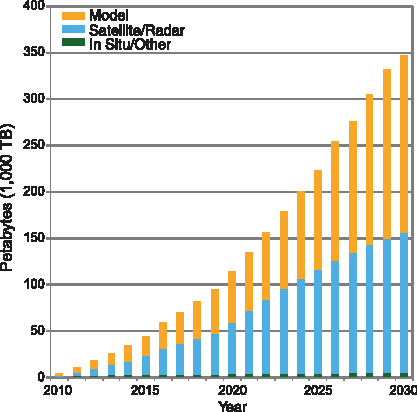
\includegraphics[width=0.5\linewidth]{3rd/overpeck_climate_2011-1_estimate-data-volume.pdf}
	\caption{Estimates of future archive volumes needed to support climate science \cite{overpeck_climate_2011}}
	\label{fig:data prediction climate}
\end{figure}

\paragraph{CMIP Archives.}

Globally coordinated Coupled Model Intercomparison Projects (CMIPs) are carried out at multi-year intervals, and involve many groups world wide running the same experiments and sharing data. With time the model resolutions increase, and so also do the number of experiments, the number of realisations of those experiments (the "ensemble size"), and the number of groups involved.

The influence of these factors can be seen in the direct comparison of data volumes produced for CMIP3 and CMIP5 shown in \Cref{tab:CMIP_data_volume}, and early estimates for CMIP6 (starting in 2017) varied between 30 and 300 PB.

The most recent UK assessments suggest the production of 3 PB of CMIP6 data within a joint modelling consortium. Given this group is likely to be attempting one of the largest ranges of CMIP6 experiments, and around 30 modelling groups, this latest data might suggest a maximum size for CMIP6 of 100 PB, but even so, it is likely that Overpeck's global projections for climate data are going to be significant under-estimates.

\begin{table}[htb]
	\small
	\centering
	\begin{tabular}{  l | c | r | r  }
		%\hline
		Centre & Country             &  CMIP3 (TB)& CMIP5 (TB) \\ \hline\hline
		BCC              & China               &  -                 & 51                \\
		BCCR             & Norway              & 0.862               & - \\
		CCCma            & Canada              & 2.071              & 51               \\
		CCSM, CESM       & USA                 & 9.173              & 739               \\
		CMCC             & Europe (Italy)      & -                  & 158            \\
		CNRM             & France              & 0.999               & 71              \\
		CSIRO            & Australia           & 2.088              & 81               \\
		EC-EARTH         & Europe (Netherland) &    -               & 97               \\
		GCESS            & China               &  -                 & 24               \\
		GFDL             & USA                 & 3.843              & - \\
		GISS             & USA                 & 1.097              & - \\
		IAP              & China               & 2.868              & - \\
		INGV             & Italy               & 1.472              & - \\
		INM              & Russia              & 0.366               & 30              \\
		IPSL             & France              & 0.998               & 121             \\
		LASG             & China               &  -                 & 100              \\
		MICRO/MICROC     & Japan               & 3.975              & 350              \\
		MIUB             & Germany/Korea       & 0.477               & - \\
		MOHC/UKMO            & UK                  &   0.973                & 195               \\
		MPI              & Germany             & 2.700              & 166              \\
		MRI              & Japan               & 1.025              & 269              \\
		NASA             & USA                 &  -                 & 375              \\
		NCC              & Norway              &   -                & 32               \\
		NCEP             & USA                 &   -                & 26                \\
		NIMR/KMA         & Korea               &   -                & 14               \\
		NOAA GFDL        & USA                 &   -                & 158              \\  \hline\hline
		Total            &                     & 34.989 (TB)       & 3,108 (TB)        \\
		%\hline          &
	\end{tabular}
	\caption{CMIP3 and CMIP5  Archive Volume (Credit: LLNL/Dean Williams)}
	\label{tab:CMIP_data_volume}
\end{table}

Looking forward beyond CMIP6, we note that the data intensity of climate model calculations is falling --- for the European contribution to CMIP5, the European Network for Earth Simulation (Andre et al, 2017, in preparation) reported an average ``production data intensity'' of 150 GB/1000 core-hours of compute, and estimate that for CMIP6 this is more like 30 GB/1000 core-hours. This falling intensity is in part because of the increase in model complexity, and in part because for many models an increase in resolution requires time-steps which are much shorter; both contribute to lower data intensity.  On the face of it, this might imply that as we move to exascale, we are likely to see even more dramatic decreases in data intensity, and while that is possible, we note that compute intensity remains the same if extra compute is spent on ensemble size. Unfortunately, this means it is hard to predict compute intensity far into the future based on these figures alone.

\paragraph{Local Archives.}
\label{sec:archive_intensity}

\begin{figure}
\centering
	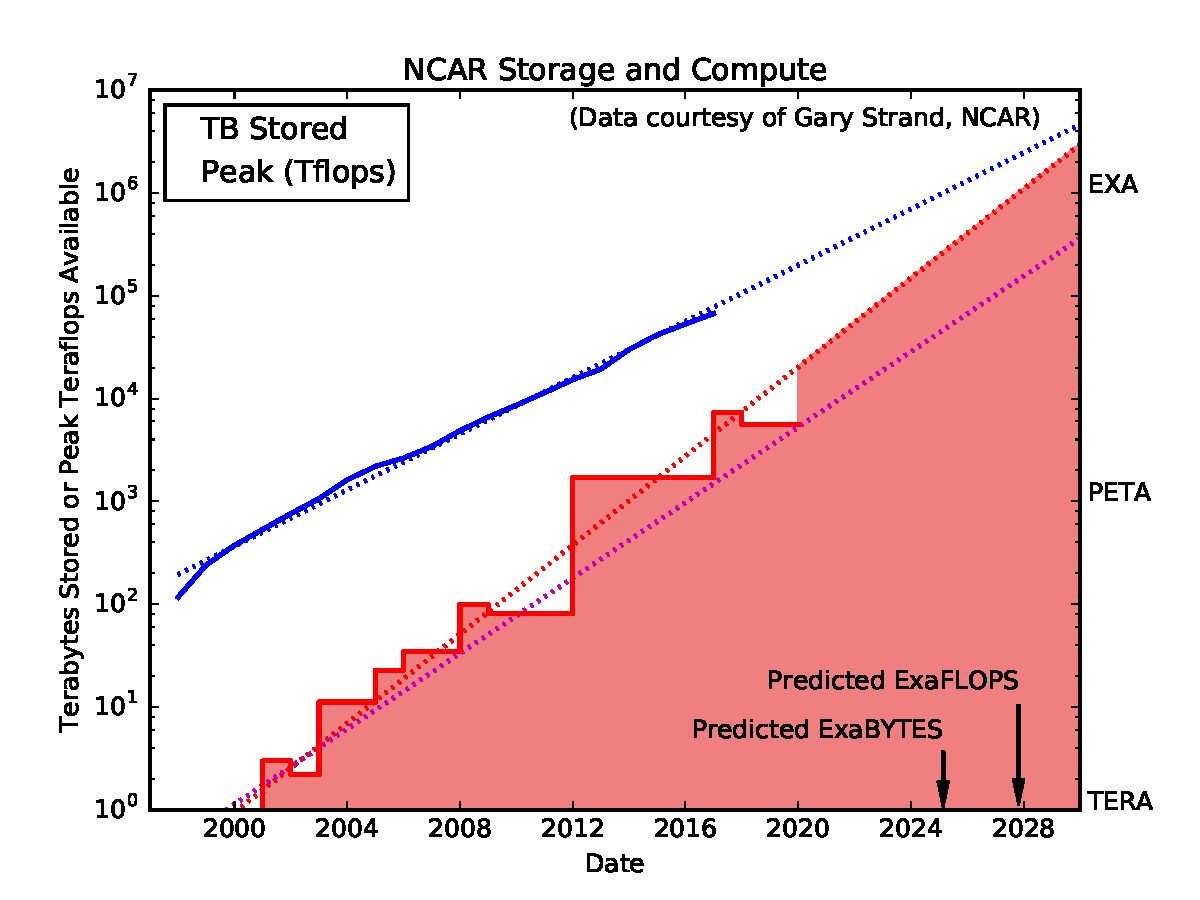
\includegraphics[width=0.7\linewidth]{figures/ncar_like_ncar.pdf}
	\caption{NCAR storage and compute. It is notable that NCAR expect to be handling an exabyte of data before they need to deal with exaflop computing.}
	\label{fig:ncar archive}\end{figure}

We are in the process of collecting local archive volume figures from key
weather and climate sites. One such site  is the US National Centre for Atmospheric Science (NCAR), who have a measurement of the total archive of data held at NCAR which can be correlated with the local compute (\Cref{fig:ncar archive}).  While the total archive includes both observation data and simulation data from other sites, it provides a useful measure of the change in data intensity, albeit via a proxy, which we here term the ``archive intensity''.  Simple back of the envelope calculations suggest that archive intensity will have gone from about 100 (TB/Tflop) in 2002 to about 10 in late 2027 when, if funding and technology were available, NCAR might be expecting to be dealing with 10 exabytes of data and an exascale compute resource.

Given that the archive intensity projection looks linear in log of the ratio, one could extrapolate the data intensity calculated for CMIP using the same assumption, which would lead to a prediction of production data intensity around 6-7 GB/1000 core hours in the mid-to-late 2020s, when we might expect it to be possible to be using exascale machines for climate science. However, on that timescale, the meaning of "cores" will have changed enough, that one might expect the data intensity in terms of core-hours used to have fallen even further.

\paragraph{Changing nature of science.}

The calculations thus far reflect the impact of extrapolation of ``business as usual''. One more important factor is the increasing scope of direct numerical simulation.  To assess how that is changing over time, we have examined\footnote{The assessment is very cursory, being based on the number of times certain phrases appear in Google Scholar citations, see \url{https://goo.gl/7q4v7H} for a complete description of the methodology.} the research literature for the use of terms which show the increasing impact of direct numerical simulation (and model inter-comparison projects) on current science. The data are shown in figure \ref{fig:citations}, and show that
\begin {enumerate}
\item  The number of papers on any facet of environmental science is growing (not unexpected, but used as a control).
\item The number of papers using direct numerical simulation is growing rapidly, but the use of DNS in environmental sciences is growing even more rapidly, at least using the proportional measure.
\item  The increase in papers which use MIP data is explosive, and one can see the direct influence of CMIP5 in the numbers.
\item Growth in observational science is slower than in numerical science, although the effect of increased availability of satellite data is apparent.
\end{enumerate}
The reason why these results are important in this context, is that they also demonstrate that data volumes are becoming an important issue for ever growing parts of the scientific community. Clearly the only way this can scale is that we replicate the data (expensive) or we improve the ability of data centres to support larger volumes and greater numbers of users!

\begin{figure}
\centering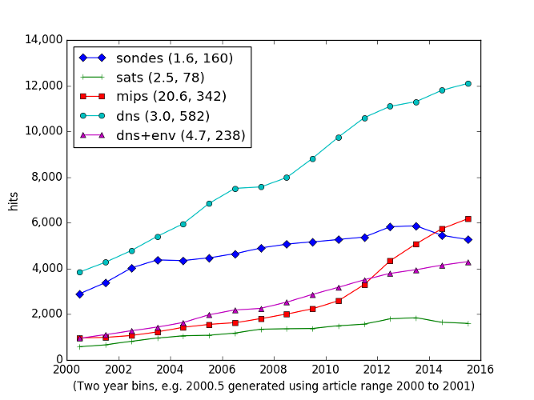
\includegraphics[width=0.7\linewidth]{3rd/google_searches.png}
\caption{The number of times certain phrases associated with direct numerical simulation (dns) or various aspects of observations (sondes, satellites) appear in the research literature. The numbers in the legend are firstly the ratio of the last couple of points over the first couple of points - a measure of proportional growth, and secondly, the gradient from a fit to the number of hits per annum - a measure of absolute growth.}
\label{fig:citations}
\end{figure}

\subsection{Technical and Financial Context}

There are four underlying storage trends that affect the acquisition, storage and utilisation of weather and climate data: 
\begin{enumerate}
\item The rise of NAND storage as a competitor for spinning disk,
\item The advent of NVRAM associated ``burst buffer'' solutions in HPC,
\item The advent of object store technology as cost effective and performant disk store, and
\item physical limits on storage and bandwidth of (spinning) disk and tape.
\end{enumerate}

These trends affect both economics and performance, and will have profound affects on workflow both in the near future, and in the medium to longer term future as 
the community embraces exabytes of data, and then, exaflop computers.  
They will also have profound impacts on cost, and as such, the architecture of future data centres will be increasingly driven by economic realities, as well, as 
received wisdom\footnote{``received wisdom'': knowledge or information that people generally believe is true, although in fact it is often false 
(\url{http://idioms.thefreedictionary.com/the+received+wisdom}). }
as to how best to exploit existing technologies. However, one of the problems with such wisdom is that it is often developed in very different environments, and may 
not be applicable to petascale, let alone exascale, weather and climate workflows. For example, while the internet giants currently handle exabytes of data, and 
deploy data mining, they do not typically handle multiple data workflows which themselves approach petascale, rather they typically handle millions of simultaneous 
megascale workflows, or handle data mining problems with gigabytes to terabytes of source data. For these reasons, their technical solutions are optimised for very 
different performance and price strategies. Hence, to examine the right computing environment for peta to exascale weather and climate workloads, basic research 
on cost/benefit ratios and possible technical strategies is necessary.

The difficulty of this basic research is compounded by the zoo of technical options available, and in particular, by the potential issues associated with multiple levels 
of storage with concomitant cache and performance characteristics. Because of this, it is often hard to estimate the cost and plan future data centres, particularly as 
we aim towards the exascale. In part this can be attributed to the limited availability and scattered nature of data on unit storage costs and performance as well as 
the lack of models for simulating the interactions between the various components found in modern data centres.  

For example, conventional hard drives provide good storage density, but decreasing ``access density'' (as capacity
increases much faster than read/write speeds). By contrast, the advent of storage class memory, non-volatile memory technologies, and flash arrays provide new opportunities for supporting high-speed access, but are expensive at scale. Similarly, tape is relatively cheap, but access latency is poor.  So it is very likely that future data centres will combine these technologies into storage hierarchies, but how does one make decisions about the architectures? 

The choice of technical options is directly related to enterprise organisational objectives, which are themselves subject to political decisions. For example, in the UK, 
the storage and analysis facility for academic climate science (JASMIN) is physically located in one part of the country (Oxfordshire), while the HPC simulation 
engines (ARCHER and MONSOON) are located in others (Edinburgh and Exeter respectively). The situation is similar for the US Geophysical Fluid Dynamics 
Laboratory (GFDL) who have their storage and analysis facility in Princeton NJ, but most of their simulations are done at Oak Ridge National Laboratory (Oak 
Ridge, TN). By contrast, the UK Met Office and the German Climate Computing Center (DKRZ) have co-located compute, storage and analysis facilities, although 
both make use of remote HPC as well. 

\begin{figure}
\centering
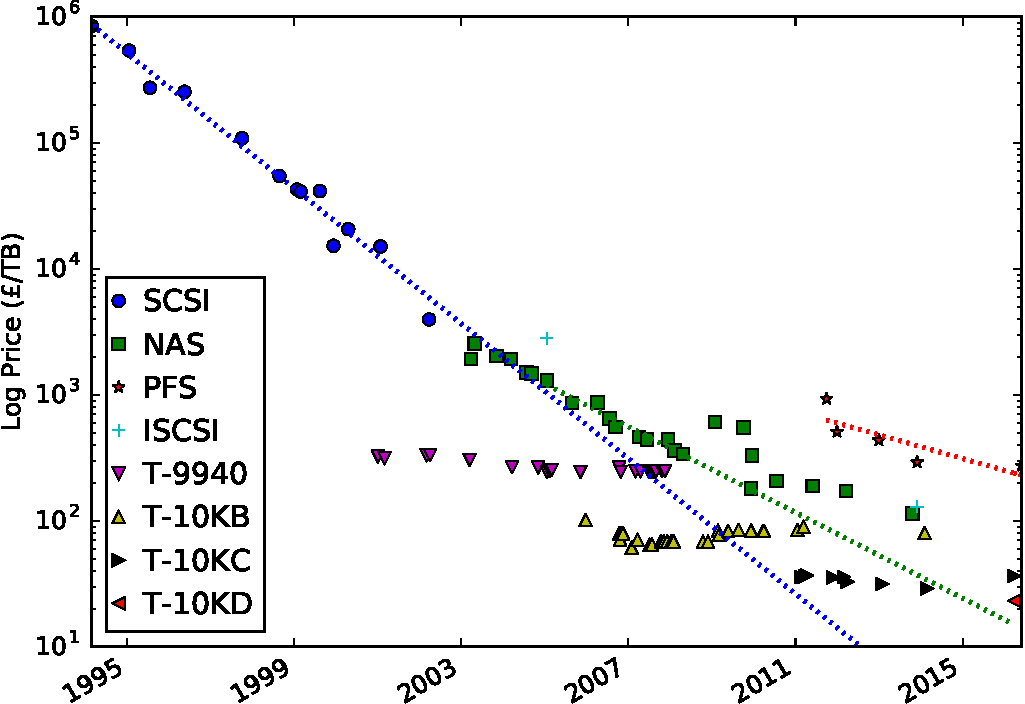
\includegraphics[width=0.8\linewidth]{3rd/kryder_2016.pdf}
\caption{Twenty years of storage costs at the STFC Centre for Environmental Data Analysis. Four distinct disk based architectures are shown, and four generations 
of tape technology. There is not enough use of ISCSI disk data to draw conclusions, but it can be seen that in the early years, the use of SCSI disk followed a linear 
trend which would have resulted in disk costing less than \pounds 1 TB in 2017 ... a trend that could not be sustained, in part because while disk densities have 
grown, the need for more and more disks has meant more and more of the storage budget needs to be spent on the kit (hardware and software) which surrounds the 
disks. The trend from the early NAS years was clearly not sustained. The advent of parallel file systems (PFS) at CEDA followed the recognition that it was not 
possible to manage or deliver the requisite performance with NAS based disk. It is too early to believe the trend in costs associated with PFS, but it is also clear that 
whatever trend might exist, will not be sustainable. The net conclusion is that the experience of disk getting cheap quickly which has provided the received wisdom 
over the last two decades that future growth in data volume will be compensated by falling costs for storage is no longer true. Disk is getting cheaper, but not as 
quickly as data volumes for storage are growing.  The advent of object store technologies will lead to a new set of data, but is unlikely to change the conclusion.
The tape storage costs also show that it is really only a change in technology that leads to substantial changes in tape media costs.
\label{fig:kryder}}
\end{figure}

In addition,  many academic/research data centres will need to support multi-disciplinary research, and will achieve economy of scale
by supporting multiple science/research areas.  A data centre run by the likes of DKRZ, the Met Office, or ECMWF can
afford to focus entirely on supporting climate research, whereas a data centre run by an organization with a wider
research base such as STFC, ORNL, or NERSC will need to support other activities, and can in fact sometimes benefit from supporting
other activities, e.g., through economy of scale.  By contrast, dedicated facilities can exploit simplifications; it can be assumed that
data contains no personal data and no sensitive data, meaning that encryption and tight access control does not need to be
 a priority within the system, and de-duplication is unlikely to be worth the investment. It might be  possible to establish workflows
 and polices which allow ``deep archival'' with data migration between cold/warm and hot storage for further analysis (and regular fixity checks).
 
In all cases there are direct trade-offs between the amount of compute and storage, and even within that, the amount and 
configuration with respect to types of usage (simulation versus analysis). 
Not all trade-offs are well understood in terms of cost/performance and scientific benefits.

One key trade-off is of course cost. Over the long-term, the fall in storage cost for disk, known as Kryder's Law has not been as linear as received wisdom expects 
(see \Cref{fig:kryder}), and while tape media costs have fallen in the long term, and over time they are generally much cheaper than disk, at times they have not 
been substantially cheaper than raw disk. These lessons: that disk is not getting as cheap as quickly as it used to, and that tape media costs are generally 
significantly less than disk, are not well known, and one of the drivers of this work will be establishing and promulgating the relevant modelling.

%
% I don't know who wrote this, but i find it offensive :-) ... as if BADC and DKRZ were not world leaders (ahead of, or 
% often in partnership with humanities and digital libraries, but certainly not behind).
%
%The multidisciplinary approach applies also to data, where, for example, humanities and digital libraries have for
%decades led the way in long term preservation and curation of data, and these activities could be brought to bear on
%climate data --- even if there were no immediate need for curation, we shall see that with increasing data volumes, it
%will become necessary to apply methodologies from preservation to ensure fixity of data.  Similar features from
%humanities (and elsewhere) which will become increasingly important include provenance, supporting processes for QA,
%and, possibly, annotations.



As well as the fundamentals of storage technology, there are other major components of systems which need to be considered. In particular,
\begin{itemize}
\item Interfaces:  The need to either develop hybrid data solutions or connected homogeneous solutions, which are fit for the workflows currently in use.  As noted 
above, this can include data migration over wide-area networks, and significant variations in how compute and storage are organised. This means storage solutions 
need to be suitable for linking to to research infrastructures that support both local and remote research institutes. They need to support data replication between 
sites (or tiers of storage), links to cloud service providers, and potentially complicated licensing regimes.  All these use-cases require standardised interfaces.
\item Automation:  Anything that doesn't happen by itself needs a human to do it.  Without automation, staff
  with the right skills and privileges need to be on hand to fix it.  While there will always be tasks that cannot be
  automated, automation of tasks helps free staff for more important tasks, and overall reduces the staff costs of the
  data centre. With increasing scale comes increasing requirement for automation, and technology choices which require
  manual intervention become unfeasible - no matter how cheap and performant they may be (it is this transition of scale, performance, and need for automation that 
led to each of the disk technology changes  shown in figure \ref{fig:kryder}).
\item Policy Support: Given the likelihood of requiring multiple levels of storage, support for effective policy management will be necessary. Support that includes 
both automatic data migration and the requirements of both system managers and users (who must be able to use their knowledge of what is important, and likely to 
be hot or cold data, to inform automatic data systems). 
  give hints or requirements on the desired features. 
\item Software:  The need for automation will also require customisation.  All storage solutions will need to support customised workflows by appropriate application 
programming interfaces. 
\end{itemize}


\section{Structure of this Deliverable} 
%%%%%%%%%%%%%%%%%%%%%%%%%%%%%%%%%%%%%%%%%%%%%%%%%%%%%%%%%%%%%%%%%%%%%%%%%%%%%%%

With the given context: growing data volumes, changing costs, new technologies, and relatively poorly available data on cost and performance, this deliverable aims to put in place the fundamentals for a more systematic approach at understanding the cost associated with storage systems. - with some of the practical work on scalability deferred to later ESIWACE deliverables. Here we concentrate on providing the building blocks for
\begin{enumerate}
	\item Coarse grained models suitable for quick estimates of cost and performance changes (models  ignorant of the actual runtime performance and temporal considerations).
	\item Detailed models and simulations that allow to evaluation of the potential and actual cost of operational facilities, including energy usage and quality of service (based on workload traces and temporal knowledge).
	\item Helping decide on future directions of research, e.g.\ by identifying obstacles to achieving the scalability required.
\end{enumerate}


\noindent The remainder of this document will be structured as follows:\\
\Cref{sec:dc_model} describes the overall data centre model, focusing on the functional architecture.
%\Cref{sec:services} goes into further detail on the data centre services, relevant to modelling individual services.
\Cref{sec:related work} presents related work and other efforts trying to improve the state of storage technologies and cost estimation in general.
In \Cref{sec:modeling} we introduce a modeling methodology to account for cost, performance and resilience of storage in data centres.
%\Cref{sec:use cases} presents a number common use cases in climate and weather applications which we will use to gauge how they are impacted by alternative storage architectures.
In \Cref{sec:evaluation} we will evaluate the costs and possible benefits when changing the architectures for a fixed budged.
\Cref{sec:conclusion} summarizes the findings and discusses future work.
We provide two appendices: a set of definitions, and a set of acronyms.

% includes goals and structure of deliverable, now one section

\chapter{Modelling the Data Centre}

\label{sec:dc_model}

In this chapter we present a range of views of data centres, beginning with some
generic requirements (\Cref{sec:generic_dc}) expressed from two different perspectives: What the data centre is for, and; What
functions are needed?

We then present a more weather and climate view of data centre requirements
(\Cref{sec:wc_requirements}) before considering additional service requirements
around packaging files, and in particular, durability (\Cref{sec:durab1}).

%%%%%%%%%%%%%%%%%%%%%%%%%%%%%%%%%%%%%%%%%%%%%%%%%%%%%%%%%%%%%%%%%%%%%%%%%%%%%%%
\section{Generic Data Centre Requirements}
\label{sec:generic_dc}

At the simplest, a ``data centre'' is a special purpose facility to handle
the production, storage and use of data. Many scientific disciplines make
extensive use of data centres, whether dedicated or shared. Nearly all
such disciplines are facing challenges in planning for the storage and use of
increasing data volumes and the consequential I/O challenges. Much of
what we discuss here will also apply to some or all of:
\begin{itemize}
\item Physics Simulations
\item Particle Physics/High Energy Physics
\item Medicine and Bio-Informatics: Molecular Dynamics
\item Neuroscience and Artificial Intelligence
\item Big Data and Machine Learning
\item Engineering
\item Astronomy
\end{itemize}

Key to understanding and modelling the requirements of the data centre are
to address the degree of specialisation, the application mix, and the impact
of the application mix on workflows and access patterns.

\paragraph{Specialization:}
The amount and nature of discipline specialisation is crucial, and will become
more so in the future as hardware becomes more heterogeneous. In the European
weather and climate community we have to deal with both dedicated and shared
facilities: dedicated to weather, climate, or weather and climate, as well as
shared with other disciplines. For example, in the UK, the academic weather and
climate community share HPC with other disciplines, but have their own dedicated
storage and analysis environment. In Germany, there is a national centre (the
German Climate Compute Center, DKRZ) which provides dedicated compute,
archive, and analysis services, to (primarily) the climate community alone.

Another key facet of specialisation is
whether or not the environment is considered operational, that is,
providing 24x7 services with hot standby --- in which case
extra redundancy is needed, to the point where in the case of the UK Met Office
and the European Centre for Medium Range Weather Forecasting, two separate
computers in two separate computing halls are used to provide such capacity.

In the work we present here, we are going to concentrate on non-operational
environments, but of necessity we address both shared and dedicated data centres.

\paragraph{Application Mix:}

The nature and range of applications supported is crucial. In particular,
from a weather and climate perspective, there are (at least three) particular
application domains to consider: \textit{simulation} (which tends to be I/O intensive
and where poor I/O performance means expensive compute nodes may run idle);
\textit{large-scale analysis} (where data volumes lead to both storage and I/O issues),
and; \textit{archive and restoration} (where discovery, latency, and volume are
all important). Within these broad categories, other important stratification
of application mix include whether or not it is interactive or batch based,
whether high end visualisation is involved (needing specialised hardware),
and whether or not it is (or could be) delivered on virtualised platforms.

In the work presented here, we concentrate primarily on the storage and I/O aspect
of the applcation mix, although of necessity this has impact on all the
computational environments.

\paragraph{Access Pattern:}
In the context of storage, a crucial aspect of consideration is to understand
the access patterns associated with typical workloads. Different access patterns
may have characteristic performance penalties, for example, where patterns can
be characterised as mainly sequential or mainly random, we can model workflow
behaviour.

In general sequential access is faster than random access, but the impact of
storage hierarchy is important. Random access to memory (and storage class
memory) carries little penalty while there is a significant latency and
bandwidth penalty with disk. Tape is prohibitively slow for random access due to
the mechanics of the medium, but after an initial latency, modern tape system
bandwidths can sometimes outperform  disk based approaches .

Often throughput can be improved by appropriate use of caches, but unless this
is automated and the automation system understands the access patterns,
throughput may not meet expectation. This is complicated by the fact that  in
many situations, a pattern obvious to an application is not understandable to
the operating system or the underlying hardware. At the same time, many
applications are ignorant about dynamics in the underlying hardware.

In the work presented here we do not have access to workflow details, so we can
only address the highest level implications of access patterns and caching strategies.

In the remainder of this section, we present a range of functional views
on the structure and requirements of a data centre. The aim is to try to identify
main drivers of costs as the data centre scales towards the exascale.

%%%%%%%%%%%%%%%%%%%%%%%%%%%%%%%%%%%%%%%%%%%%%%%%%%%%%%%%%%%%%%%%%%%%%%%%%%%%%%%
\subsection{Functional View}
\label{sec:dc_func}
\label{sec:dc_services}
\label{sec:dc_discovery}

Originally developed by the Consultative Committee for Space Data Systems
(CCSDS), the Open Archival Information System (OAIS) contains a reference model
[Lavoie] which is now an ISO standard ISO 14721:2012.  While its underlying
purpose is the data centre as an archive, we use it here as a reference for
modelling the data centre's \emph{functional} responsibilities.
Figure~\Cref{fig:dc_arch} shows an extension of the OAIS model, which we use
as a focus for discussing functional requirements.

\begin{figure}[]
  \centering
  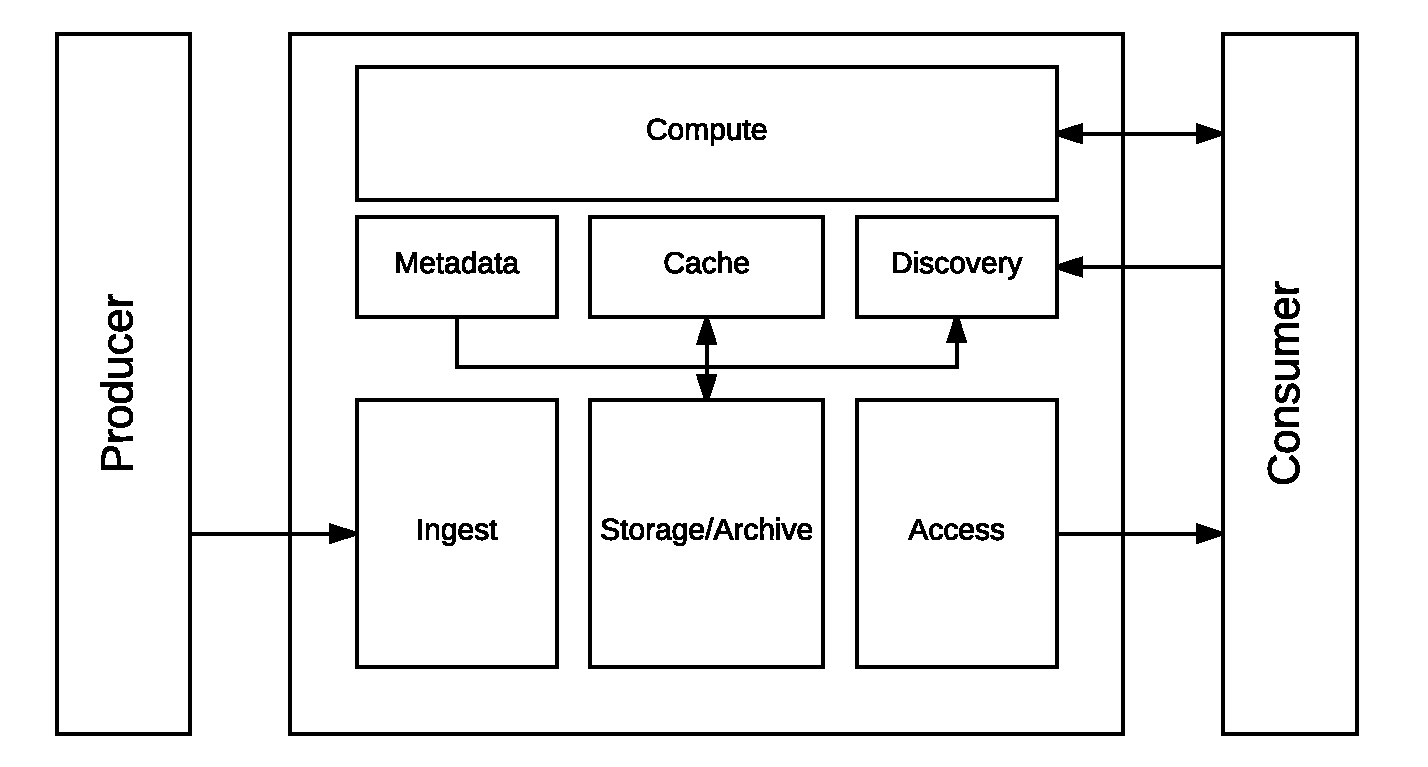
\includegraphics[width=0.6\linewidth]{figures/datacentrefunctional.pdf}
  \caption{Functional architecture of data centre. }
  \label{fig:dc_arch}
\end{figure}

We begin by
concentrating on the relationship between the compute, the storage/archive,
and the network.

% The role of modelling (stochastic and computational) and simulations

% Underlying fabric – covered below (Data Centre Implementation)

% (XXX - fixme: A data centre is not just about data, it is also about compute.  Note distinction in implementing “data intensive” HPC
% compared to “compute intensive” HPC (and supercomputing).)
\paragraph{Compute:}
Very broadly speaking, there are two kinds of scientific computing:
\textit{simulation}, which takes a set of parameters and generates some kind of
output, and \textit{analysis} which takes data and processes it. Received wisdom
has it that analysis generally reduces data volumes (as in statistics, big data,
etc.), whereas simulation increases data volumes. However, in weather and
climate this is not always the case. Many analysis data ``reductions'' create
extra data which has to be differenced from the original data (thus multiplying
up data volumes), and scientific post-processing can often create much more data
than was input (as is the case with an ``afterburner'' approach to producing
diagnostic variables from a weather or climate simulation).  However, there is
one crucial distinction in play: generally simulation compute requires many
(thousands) of compute cores which cannot be idle while waiting for I/O, whereas
analysis compute is generally much smaller, and schedulers can more easily
afford to idle jobs on I/O wait. However, even in analysis compute I/O wait
cannot be excessive, and in fact methods for parallelising I/O are sometimes
even more important in analysis than simulation, and the data centre needs to
provide appropriate hardware support.  Sometimes these two forms of computing
are differentiated by the notions of High Performance Computing (HPC) for
simulation and High Througput Computing (HTC) for analysis computing.

In both cases, coupling data storage with computing resources is necessary: the
alternative of moving large volumes of data repeatedly is expensive and time
consuming, so it is essential to have compute %  (see \Cref{sec:dc_lifecycle})
capability ``close'' to the data (of course it is also essential to be able to
move data around.)

\begin{itemize}
\item Staging: Compute needs to be supported via data staging (job doesn’t
run till data is ready) and ingest (application doesn’t finish till data has
been acknowledged written to storage and/or till the requisite number of replicas
have been created – the durability target has been reached). % (section \ref{sec:durability})
\item Networks: Compute is typically supported on fast interconnect within the data centre,
but the topology can be sensitive to the balance of analysis/simulation and
the need for inter-node communication.  Where simulation and analysis
environments are separate attention to firewall and wide-area network
bandwidth issues is important.
\item Caches:  Both HPC and HTC can benefit from several caching environments
(see Future/Technology) ([Dosanjh],
pp. 35-36, and [Quan et al], pp. 14-18). Application level caching can be
supported with nodes with extra memory, or through NVRAM/SCM (i.e. jobs are
running as a part of the application but their main purpose is to cache data for
fast access by other jobs, or provide dedicated I/O).  Specialised
machines or machine architectures may be needed (or be beneficial) for some
types of applications, thus incurring extra costs.
\item Compute Hardware: The type of compute hardware required may differ
significantly between simulation and analysis, allowing very different
system configuration, quality, and cost to be deployed.
\end{itemize}

\paragraph{Ingest:} Storage can provide different features or different
qualities of service (such as durability and availability), and it is important
to match the user requirements against the features provided by the data centre,
in order to ensure that the correct service is delivered in the most cost
effective manner.  It follows that the user must be able to specify the service
requirements upon ingest; this could happen either via the user specifying
support in policy terms or via directly addressing different parts of the
datastore, e.g.\ via a file path or an object store bucket.

In particular, upon ingest into many types of data centre storage, users ought be
able to:
\begin{itemize}
\item request suitable data storage policy parameters, for example
durability and availability --- via policy terms which might address how
many copies of data were kept and whether it was necessary to have the data
nearline or in cold storage.
\item provide hints as to how data is likely to be recalled, or what parts
of data might be recalled together. If data is stored inefficiently, or
it is necessary to recall larger chunks of the data than are needed, then
recall time may be longer by several orders of magnitude --- which may
be expensive in resources (including potentially human resources).
\item receive notification when the data service goals are reached, e.g. for
durability, that data has been written to the required number of tape copies, s
so that the client can delete its data.
\item employ suitable endpoints to initiate and manage data ingestion (e.g.
browser/command-line/API) via suitable services (e.g. GridFTP etc).
\end{itemize}
(And recognising that data ingestion is something that both happens on the
boundary of a data centre, and within data centre workflows, all
ingestion characteristics also need to be visible to local users.)

In this context, \textit{Recall}, is an important requirement, allowing
users to exploit any storage hierarchy, including from tape. In particular
users should be able to
\begin{itemize}
    \item request data from slower storage and where latency is an issue, be
notified when it is ready, ideally with an estimate prior to recall it of how
long it would take (based on bandwidth and contention),
    \item pre-stage data for batch jobs, so that schedulers can efficiently
    manage compute and storage resources (and so that users don't pay for CPU
    wallclock when the jobs are waiting for the data).
\end{itemize}

\paragraph{(External) Access:}
Users need to be able to export data, and external users may need to access data centre
services to extract data. Suporting export and extraction requires attention to data
discovery, data transfer/service provision, and network bandwidths. In particular,
\begin{itemize}
        \item  Data centres must provide data replication facilities, and
        \item Support high bandwidth network transfers, which may involve
        customised network environments (e.g. see \Cref{sec:dmz}).
\end{itemize}

Such replication and transfer services may need bespoke customisation if the
storage hardware and software doesn't directly support them. For example,
GridFTP \cite{GridFTP}, is a highly efficient open standard data
transfer protocol, which every year transfers hundreds of petabytes of science
data globally, and it forms the foundation of the Globus file transfer services.
Thus, having GridFTP endpoints in the data centre is useful for many customers.
However, when adapting a GridFTP endpoint to
something other than a POSIX filesystem interface, typically some development
work is needed, particularly when good performance is desired (i.e., the service
can take advantage of the striping.)  STFC has put effort into adapting GridFTP
to CEPH, based on original work by CERN, but services can also be bought:
SpectraLogic's Black Pearl supports GridFTP out of the box.  In costing terms,
it becomes a tradeoff between staff (development) or capital (Black Pearl.)

Bespoke services obviously become more expensive, as they need to be integrated
with existing data services and they need to be supported.  Integration is not
necessarily a one-time cost, as upgrades to services may require updates also to
the integration between the services.

\paragraph{Discovery:} Clearly at scale, it is not possible for human intervention
to find and aggregate files for analysis, extraction or replication.  All services
need to be machine interrogatable as to capability and content, and all hardware
needs to support these characteristics. This means in practice that data centre
costs need to include both the software and hardware costs of metadata systems.
It also means that authorisation, authentication and access need to be automated
and data permissions need to be able to be delegated through all levels of the
storage hierarchy.


\subsection{Security}

A data centre has to have security, both physical (access control for authorised
personnel, building security, flood and fire protection) and virtual
(firewall, authentication, possibly at-rest and in-flight encryption).  Of
course, physical security incurs a cost, both in the initial investment and
in operation; likewise staff may need to be vetted and trained in security.  Of
particular importance is that virtual security features do not impede the
performance of data transfer and access: for this reason, unless it is
absolutely required, encryption is switched off for scientific data transfer
(obviously this creates a certain risk of leaking information or a malicious
man-in-the-middle modifying data in flight, but those risks are generally low
and can be accepted without further mitigation).  A data centre must usually
cater to different security requirements,  a typical setup will have mutual
authentication and encryption on the control channel (cf.\ \cite{GridFTP}) and
(only) data channel authentication.

\section{Specific Requirements}
\label{sec:wc_requirements}

Thus far we have looked at generic requirements, albeit from a weather and climate
perspective. Here we focus more on data centre concepts and components of
particular relevance to existing weather and climate.

\begin{figure}
    \centering
    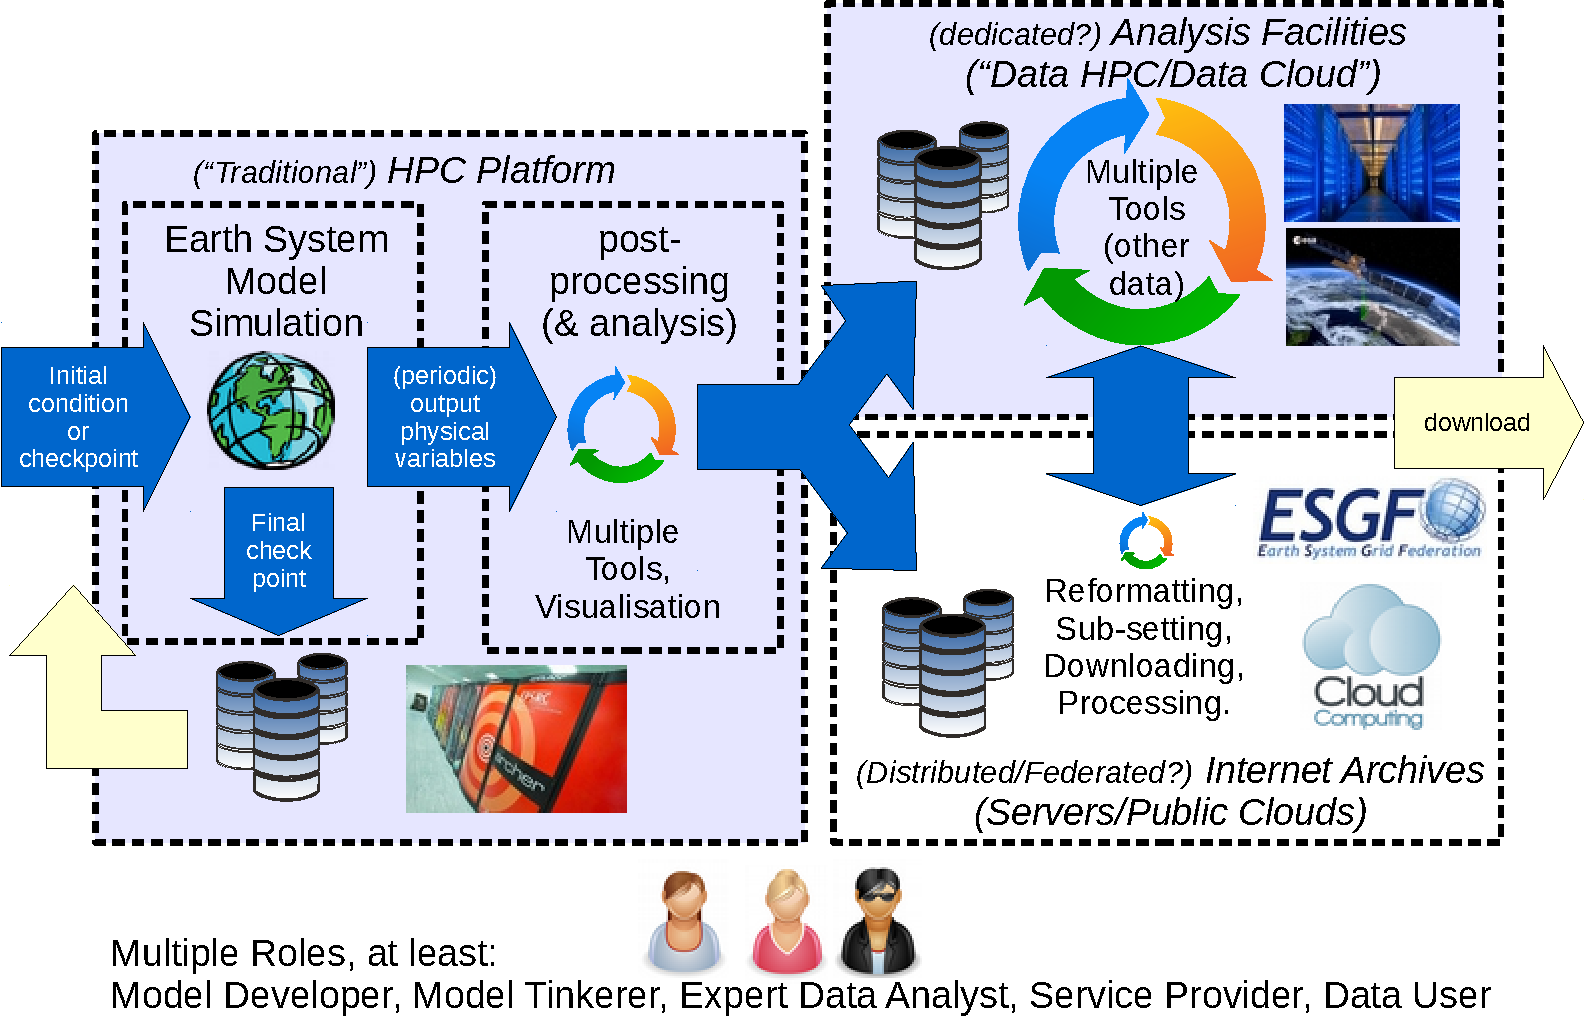
\includegraphics[width=\linewidth]{3rd/workflow-crop.pdf}
    \caption{Characterisation of key elements of weather and climate workflows.
    There are three logical ``data centre'' components, which may or may
    not be physically co-located, and which need to support a range of roles.}
    \label{fig:wc_workflow}
\end{figure}

Figure \ref{fig:wc_workflow} provides a schemtic of the three key
data centre environments from the perspective of weather
and climate workflows:
\begin{enumerate}
    \item An \textit{HPC platform} where the key aspects of the
storage system need to support the fast loading of simulation initial conditions
across thousands of nodes, as well as checkpointing throughout and at the end of
the simulation. Also throughout the simulation is the necessity to write data
out for post-processing and later use: this process generally requires reshaping
of variables, and involves significantly more data handling than the
checkpointing. The storage system associated with this platform generally needs
to support post-processing directly after the conclusion of the run, an activity
which might include multiple software tools and different ways of accessing the
data than were use to write it. Sometimes this post-processing might include
writing most of the data to an archive medium (slower storage tier, such as
tape), for later recall.
    \item An \textit{analysis facility} where users are likely to
    be comparing and contrasting model simulations and observations, and
    so data volumes in some workflows can be significantly larger
    than in any one model simulation experiment. At the same time, software
    is less likely to have inherent parallelisation, although some tasks
    will be able to exploit massive parallelisation in time (for exmaple,
    applying the same algorithm to all timesteps in model output for example).
    This means the storage and I/O systems will likely need to handle even higher
    bandwidths and througput than the HPC platform, and certainly larger
    volumes of accessible data.
    \item An \textit{internet accessible archive} (for example,
    the Earth System Grid Federation, ESGF) from whence users
     can download data to external sites, and where they might potentially
     be able to do either a limited amount of server-side processing, or
     potentially even deploy their own analysis environments on cloud
     computing which has direct acess to the data. Here the storage system
     needs to be well connected through secure interfaces to wide
     area networks, and may have a range of data handling services, from
     GridFTP endpoints, to local provision of ``infrastructure-as-a-service''
     (IaaS) cloud.
\end{enumerate}

There are some distinguishing characteristics of these three environments:
\begin{itemize}
\item The number of users: A relatively small number are responsible for
developing and modifying (tinkering with) models on the HPC platform, with perhaps
hundreds to thousands working in the analysis environment, and with the largest
centres (such as DKRZ and STFC/CEDA) supporting tens of thousands accessing the
outward facing archives. (The number of users will have implication on the
way that storage, services and I/O are organised and scheduled.)
\item The I/O and interconnect subsystems in the HPC platform are likely to need to deal with considerable inter-process communication, while those in the dedicated
analysis facility are more likely to have to deal with simultaneous I/O without
inter-process communication (at least with existing analysis algorithms, future
algorithms may become more complicated as analysis users realise they have
to find new ways of exploiting data parallelism to have acceptable times to
solution - acceptable not only for the user, but also in terms of time
exploiting resources). It is unlikely that much parallelism can be deployed
in the internet archive, unless it is deployed in a public cloud, since most
sites will not be able to deploy enough resources to support large numbers of
users with simultaneous, synchronous computing demands.
\item The amount and complexity of systems to protect users from each other
and from both deliberate and inadvertent data destruction will vary considerably across these domains: on the HPC platform, it can be assumed that all processes
can run with minimal access control beyond constraining ``access to the system''.
By contrast, codes running on an IaaS cloud could do anything, and no write/delete
access should be possible for \textit{anything} running on an untrusted IaaS system. This has implications for the nature of the storage interfaces and their complexity.
\end{itemize}

Of course, in some communities, all three of these environments are deployed
on the same hardware platform and/or in the same machine room. However,
in any modelling of the data centre, one may need to separate out the
systems needed to provide these services (which may also include
replication between environments and storage tiers, as already noted
in the generic reuqirements).

%%%%%%%%%%%%%%%%%%%%%%%%%%%%%%%%%%%%%%%%%%%%%%%%%%%%%%%%%%%%%%%%%%%%%%%%%%%%%
\section{Supporting (Local) Compute Applications}
% moved here from the chapter on related work ...

We have seen the necessity for supporting local compute (as opposed to
primary HPC), whether for post-processing with the HPC, or in dedicated
analysis facilities.

This will have implications for the types of storage necessary:
\begin{itemize}
\item Primary Supercomputing Input/Output, to support:
\begin{itemize}
    \item Input and Output Checkpoint data
    \item Primary Scientific Outputs
\end{itemize}
\item Secondary Input/Output, to support user programmes, but perhaps
with lower I/O bandwidth requirements than primary output.
\item Read Only Primary Data --- data is only read and not updated (although
metadata may be updated),
\item Primary and Secondary I/O storage may support one or both of :
\begin{itemize}
\item Scratch space, and
\item Permanent storage (with assigned durability --- \Cref{sec:durab1}).
\end{itemize}
\item Primary source code storage (ususually with full backup),
\item Append-only storage (e.g. for logs)
\end{itemize}
It may make sense to support these data types differently, depending on
scale, number of users, and typical workflows. Supporting different data
types in different ways is also a logical extension to the general support that
HPC and supercomputing operators give to their application developers: it is in
the interest of both to have applications run as efficiently as possible, and
applications often have to be developed to take the infrastructure into account
(for example, local cache, storage blocks/stripes, parameters for parallel-HDF.)

In addition, metadata storage must be supported not just to aid the application's
use of the data via metadata but also to record the provenance of the derived
data:
\begin{itemize}
\item which algorithms were run and with which parameters,
\item who performed the calculation,
\item which versions of programs and libraries were used,
\item which compute architecture,
\item licences and access permissions for the derived data (which may derive from the licences of the input datasets, possibly in a way which needs to unify different licences on input datasets)
\end{itemize}

\section{Additional Service Requirements}

This section adds further data service requirements, some of which we do not
expect to have implications for initial data centre models such as those
presented in later chapters, but which may both have implications in some future
model which includes service costs and be relevant to other aspects of ESIWACE
exploitability.

\subsection{Packaging and Metadata}
\label{sec:packaging_and_metadata}

 Existing data centres in weather and climate
are primarily based on handling files, which may or may not have internal
metadata content.  However, all centres have developed their own systems which
manage file content, from MASS at the UK Met Office, to MARS at
the European Centre for Medium Range Forecasting. STFC/CEDA expoit bespoke
systems to interface between file based disk, and the CASTOR tape system.
One key part of these systems is that data being migrated between storage tiers
is not necessarily left untouched, tier migration might include:
\begin{itemize}
\item Changes to data granularity, for example
\begin{itemize}
    \item Small files can be packaged up into a shared container (e.g. tar files),
    or
    \item Large files may be pre-chunked or re-chunked to allow optimal
    storage and retrieval along different axes than the original organisation.
\end{itemize}
\item Pool management, where data systems have the notion of pools, datasets
may need to be managed in contigous pools, which may themselves have
specific criteria (e.g. managed for read/write and automatic backup/delete or for write once, two copies, etc).
\item Metadata management, to allow data discovery against both the
original organisation, and the new organisation.
\item Usage Accounting, to support both
\begin {itemize}
\item the use of appropriate use of storage tiers and storage migration (autmatically
making hot data more accessible and moving cold data to cheaper storage but
still available with greater latency), and
\item reporting on data usage, for publication and management metrics.
\end{itemize}
\end{itemize}
All hardware systems will need to support some of these packaging notions,
with consequential implications for software, and data centre costs.

%%%%%%%%%%%%%%%%%%%%%%%%%%%%%%%%%%%%%%%%%%%%%%%%%%%%%%%%%%%%%%%%%%%%%%%%%%%%%%%
\subsection{Durability Implications}
\label{sec:durab1}

It should not come as a surprise that storage with higher durability comes with
a higher cost.  The most basic way of implementing higher durability is LOCKSS --
Lots of Copies Keeps Stuff Safe -- meaning keeping multiple copies of the data,
but keeping $N$ copies reduces the available storage space by a factor $N$.

We discuss this further now, and not in later chapters on cost modelling, since
from the point of view of costing a data centre, we can treat the cost
implications arising from durability requirements as simple multiplicative
factors which impact on storage choices in signifcant ways.

If the loss of a single replica has probability $q$ (in time interval $T$), and we keep $N$ copies,
then the probability of losing all $N$ (equivalent) copies in the same time
frame is simply $q^N$, provided the losses are independent\footnote{Which
is not always a good assumption, for example,
there have been cases where vibrations in disk arrays have caused correlated
disk failures, so it is necessary to actively manage the independence
of the data copies!} of each other.

As a simple model, if the durability ($1-q$) of a single copy of the file is
$0.97$ (in $T$), and a durability of 0.999 is desired, then
$N=\lceil\log(0.001)/\log(0.03)\rceil=2$ copies are needed.
For a durability of $1-10^{-5}$, we would need
$\lceil-5\log(10)/\log(0.03)\rceil=4$ copies. When the time interval
is short, $q$ is relatively small, and $N$ can be small too. When the
time interval becomes long $q$ is inherently greater, and so the durability
falls without extra copies.

Similarly, with many files, the probablility of some data loss scales
at least\footnote{Actually it scales worse than linearly since
many modes of data loss will take out many files at once.} linearly with the
number of files.

It follows from the impact of time intervals on $q$, that the probability
of data loss in any given period $T$ can be reduced by \emph{detecting} the loss
of a copy, within that period, and before further losses occur. That is,
be subdividing the period $T$ into shorter periods $t$, and checking
for file integrity at interval $t$, and where necessary recovering files from
the additional copies.  This has the immediate impact of a direct reduction
on the number of copies needed to maintain acceptable durability for $T$.

This impact can be quantified: for given $q$ and $T$, the probability of
data loss in $t$, $q_t$ is simply $qt/T$. The impact on durability and number
of data copies is straight forward.

Such interval checking can be managed or un-managed. In the latter case it might
occur from normal user data access - when a user attempts to open a primary copy
of data file, and it is found to be bad, a secondary copy can be used (and the
primary copy quietly replaced in the background), but only if it too is bad.
However, this does not provide reliable durability, not only are not all copies
checked (backup copies are only checked if the primary copy is bad), but not all
files are checked. By contrast, if \textit{every} copy of \textit{all} files are
checked for integrity periodically (possibly on a rotation basis), it should be
clear that the durability of the file is improved as the risk of the loss of all
copies of a file in that time is significantly smaller than it would be over
longer time periods.

Periodic detection and repair of data damage can happen in a number of ways.
Live system monioring at the disk and file system level can detect and repair
data loss in many ways, from hardware health monitoring leading to proactive
data  copying (e.g. when drives start showing errors), to the use of RAID
systems which can detect and repair data at the block level.  File systems can
add further automatic fault detection and repair. For example, HDFS replicates
blocks, and it can be configured to replicate blocks across boundaries so the
blocks are not stored in the same drive/array/rack, but copied explicitly to
another for resilience (up to the desired number of copies.)  In the case a
server needs removing from a HDFS infrastructure, instead of the conventional
draining of the server (by moving data from it to other servers), one simply
disconnects it and lets HDFS rebuild the missing copy of the blocks from the
remaining ones.

A similar benefit arises from erasure coding (see definition on page \pageref{para:erasure_codes}). Typically, systems using erasure encoding include
extra complexity, and need more CPU since erasure encoding is handled software
in the storage system - but it can attain higher durability for data since the extra copy overhead is lower.

In any case where automatic rebuilding of data is occurring, the system may be at higher risk of data loss while this takes place, so any system which can minimise this time is advantageous. For example, if it is necessary to drain data
from a server before making additional copies, or rebuilding, this increases
risk over strategies that do not need this initial step.

One key method of minimising durability cost is to used tiered storage, where
lower cost, lower latency media can be used for replicas, since latency is
unlikely to be an issue where recall is in response to automatic periodic
fixity (next section) checking.

The cost of durabilty is obviously smaller if data is compressed or deduplicated
before storage, but the former depends on being able to achieve signficant compression ratios, and has high CPU costs, and the latter is not expected
to work well for weather and climate data - at least at the file level, interesting results have been reported for deduplication of information within data \cite{gmd-10-413-2017}.

\subsection{Durability Requirements}

The importance of durability leads to a set of requirements that are
exposed to system managers (as opposed to internal durability requirements
such as fufilling RAID or erasure encoding related data replication).

\paragraph{Levels of Durability} It must be possible to define and implement different levels of durability.
  \begin{itemize}
      \item It must be possible to communicate available levels to those
      storing data, and it must be possible for such users to choose
      specific levels of durability.
      \item It should be recognised that it may be necessary to manage replicas across sites as well as within a data centre.
  \end{itemize}

  \paragraph{Replication:} Durability may require replication, both within and
  between data centres.
    \begin{itemize}
    \item The placement of the replicas must be aware of the physical location of each replica, in order to maximise risk independence of replicas.
    \item It follows that the replication mechanism must be
    \begin{itemize}
    \item able to ascertain which medium holds a given data set, and
    \item able to determine media which are independent (in terms of risks of failure) of any current location of replicas, and
    \item target the placement of additional replicas to these individual media.
    \end{itemize}
    \end{itemize}

\paragraph{Fixity and Catalogues:} It must be possible to evaluate data integrity.
\begin{itemize}
\item It follows that data must be written and stored in a canonical form which has a well-defined length and can be
  checksummed\footnote{If the data is a file or an object consisting of a sequence of bytes, one would simply checksum
    the data as a sequence of bytes, but other data – JSON, XML, for example – would need to be rendered in a canonical form before being checksummed.}.
  \begin{itemize}
  \item Appropriate checksum technologies should be used (typically file size
  is not enough, tests for bit corruption should also exploit digital hash
  technologies such as MD5 checksums).
  \item Within weather and climate, it is unlikley that provenance fixity
  (e.g. digital signatures) will be necessary.
  \end{itemize}
  \item The length, checksum, storage location of data and replicas, and other relevant metadata, must be stored in a catalogue or other metadata system so this metadata can be preserved and accessed independently.
  \item It should be possible to rebuild the metadata catalogue from the media.
  \item It must be possible to determine the time and status of the most recent integrity check.
  \item It must be possible to check every replica of the data independently.
  \end{itemize}

\paragraph{Preservation Checking:} must be carried out at regular intervals,
which involves evaluating all copies of all data against the fixity catalogue.
This involves:
  \begin{itemize}
  \item Ensuring data is checksummed at ingest.
  \item Evaluating fixity when migrating between storage tiers.
  \item Periodically ``waking up'' data and checking fixity using a pre-defined
  period calculated from the durability requirements.
  \item Monitoring storage media, and taking appropriate action (e.g. monitoring
  disks for bad blocks and/or read/write errors and retiring media with poor
  statistics).
  \item When random failures are found, an investigation and recovery process (that
  is as automatic as possible) should be initiated so that:
  \begin{itemize}
      \item Corrupt data can be replaced,
      \item Statistics of media reliability can be updated,
      \item Where necessary, media can be replace.
      \item Recovery times can be evaluated.
      \item Users and administrators can be appropriately alerted.
  \end{itemize}
  \end{itemize}


%%%%%%%%%%%%%%%%%%%%%%%%%%%%%%%%%%%%%%%%%%%%%%%%%%%%%%%%%%%%%%%%%%%%%%%%%%%%%%%
%%%%%%%%%%%%%%%%%%%%%%%%%%%%%%%%%%%%%%%%%%%%%%%%%%%%%%%%%%%%%%%%%%%%%%%%%%%%%
%%%%%%%%%%%%%%%%%%%%%%%%%%%%%%%%%%%%%%%%%%%%%%%%%%%%%%%%%%%%%%%%%%%%%%%%%%%%%
\chapter{Related Trends}
\label{sec:related work}

In the previous chapter we introduced the key requirements of weather
and climate date centres. This section provides an overview of
complementary elements of the data centre status quo and introduces related trends.

\section{Data Centre Evolution}
\label{sec:related work/data centre evolution}

We may here look at the evolution of the data centre itself, or we may look at
the evolution of the use of the data centre.  The former will focus on the data
centre from its own perspective --- how does it provide services to its users,
how do its services and features evolve with time, whereas the latter will look
at how the users do the work that traditionally involves data centres: this work
could, in principle, change to involve more distributed and collaborative
working (\`la wikis or VREs), use of clouds for on-demand services, truly
distributed computing \`a la BOINC, and of course desktop computing.
Nevertheless, the principal focus of this document shall be the use of the data
centre itself for high-end data storage and data processing, because, as we
shall see, none of the other options can currently --- or in the near/medium
future --- provide cost effective alternatives.


% A bit of history plus recent and future.

In looking at the evolution of data centres, it is useful to look at where the
evolutionary pressure comes from. We have introduced some of those drivers in
the introductory chapter, but there are others that come naturally, with growth
in data storage requirements (and associated bandwidth requirements),
accompanied by co-evolutionary technological advances -- increased storage
densities, higher bandwidth networks, ``cloud'' computing.

At the same time, we are seeing evolutionary drivers both in the commercial
world --- the exabyte datacentres of Google, Facebook --- and those of the
academic world where also HEP, astronomy, and biosciences have increasing needs
of data ``solutions'' and are pushing for those needs to be met, often in
different and incompatible ways due to differences in history and culture.  In a
topological (or, more precisely, networkological) sense, data typically need to
be close to the CPU that processes the data, so typically a data centre would
provide ``its own'' compute infrastructure (e.g. in a commercial CSP, data
access within the same regional data centre is free but may cost if data is
accessed from another region.)  Another important networkological factor is the
connections to research networks; for example both Amazon's and Microsoft's data
centres in Ireland are peered with the JANET, the UK research network.
Similarly, geographical and legal constraints can affect the placement of data,
particularly if the data can contain personal information which is subject to
data protection regulations or other national constraints.

Beyond this, we have constraints arising from society and the environment:
\begin{itemize}
\item the costs of operating a data centre %(section~XXX)
\item the ``greenness'' (power, cooling, CO2 emissions and other pollution, the environmental friendliness of the hardware in
construction, delivery, operation, and disposal),
\item physical security and access control,
\item location (e.g. protection from natural disasters: flooding, earthquakes, etc.),
\item space constraints (in particular, can it be extended),
\item personnel security
\end{itemize}

Unsurprisingly, setting up a datacentre from scratch is a significant investment --- building, security, tape store,
storage and compute nodes, power, cooling --- and it is necessary also to consider alternatives, namely:
\begin{itemize}
\item Use of (public, commercial) cloud data centres.
\item Co-location --- use an existing (usually commercially operated) data centre.
\item Shared data centre --- different research domains share the use of a data centre (one of the differences between
  this option and co-location is that the boundaries are more flexible in the shared data centre, and resources can be
  shared between users or be loaned from one user to another).
\item In-house private resources --- the ``traditional'' university department approach where each department runs its own
  storage and computational cluster.
\end{itemize}

In practice, a data centre ``solution'' could be a hybrid, combining several of
the above resources (see~\Cref{sec:cloud}).  Building hybrids makes it even more
important to have common interfaces based on open standards with interoperable
implementations.

In building the data centre itself, there are also several options, as we shall
see in the section ``data centre implementation'', below.  Here, other factors
come into play, too: the overall capacity of the data centre in terms of
physical space, power, cooling, electricity supply and backup (UPS and
generators).

%%%%%%%%%%%%%%%%%%%%%%%%%%%%%%%%%%%%%%%%%%%%%%%%%%%%%%%%%%%%%%%%%%%%%%%%%%%%%
\subsection{Commercial CSPs and their Services}

%\todo{references!}

The large public cloud service provicers (CSP)s (see \Cref{sec:cloud}) (e.g.
Google, Amazon, Azure, Rackspace) and social media networks (Google again,
Facebook) run large data centres, and often develop their own technology or
software to support them (e.g. Microsoft's Project Catapult, the Google File
System), or to support the use and analysis of the data (e.g. Google's Drill).
These data centres have been designed to be able to provide high resilience
services --- with presence in different regions of the world and the ability to
replicate data both between regions and also to provide multiple copies within a
single data centre.  Users can choose the level of replication suitable to their
data; obviously they also then pay for the service access.  Similarly, special
use cases can be supported: a content distribution network may be optimised for rapid
location-independent delivery of data to users, data analysis and ``mining''
facilities, data traffic and network management, data ``market places,'' etc.

For an academic data centre, it may be best to leave many of these additional
features to the commercial CSPs and let users procure their own cloud resources
as needed; it would then suffice to provide interfaces that let users move their
data to/from commercial clouds, and perhaps also to provide data movers
compatible with the more common commercial cloud interfaces (the latter requires
that users are able and willing to delegate their access rights to the data
mover.)  The usage model would then be that data would remain in the academic
data centre, but users could, when they need these extra services, move the
data, or ask to have the data moved, to the public cloud where the additional
services could be provided.  For some research disciplines, certification of
data centres becomes important --- this is particularly notable in
bioinformatics, where users are not keen to pursue the details of the security
implementations but know that they need the security, both physical and
operationally.  In this case, relevant data centre certifications become
helpful; such as [SSAE16] (formerly known as SAS70). Even if a full audit is not
performed, the certification may serve as a useful checklist.

%%%%%%%%%%%%%%%%%%%%%%%%%%%%%%%%%%%%%%%%%%%%%%%%%%%%%%%%%%%%%%%%%%%%%%%%%%%%%
%%%%%%%%%%%%%%%%%%%%%%%%%%%%%%%%%%%%%%%%%%%%%%%%%%%%%%%%%%%%%%%%%%%%%%%%%%%%%
\section{Recent and long-term trends for storage technologies}
\label{sec:related work/trends storage}

Various studies regularly revisit the technological progress in storage and
compute resources. Vendors, customers and operators likewise are motivated to
perform market analysis to align their spending and business strategy. A general
trend is the increasing performance discrepancy between storage and compute
hardware. \cite{julian_m._kunkel_exascale_2014} notes that processor speeds over
a 10 year time frame increased by a factor of about 500 with disk capacities
keeping up only slightly slower with a factor of 100. So while we have
technologies with the necessary capacity to store most of the computed data, we
lack the technology to store data at the same pace it is created. For example in
the last 25 years, processors speeds improved by roughly a factor of a million.
In the same time frame storage speeds only achieved a 1200x improvement. This discrepancy is exacerbated by the increasing archive intensity noted in section
\ref{sec:scientific context}.

Similarly others compared different storage technologies.
\cite{fontana_impact_2013, decad_impact_2013} analyzed the cost development of
NAND, disk and tape storage media from 2008 to 2012. The authors compared the
units and petabytes shipped, the areal density in bits per inch as well as the
generated revenue and dollar price per GB. HDDs are leading in terms of globally
shipped PB and generated revenue. In terms of areal density HDDs continue to
outperform NAND (second) and tape. But higher density tapes have been already
demonstrated, promising capacities of up to 200TB per tape in the near future
possibly surpassing NAND in areal density. Natural disaster or change in
production facilities also had an observable impact on HDD sales e.g. following
floods in 2011 in Thailand (also see our figure \ref{fig:kryder}). While disk
and NAND benefit from economies of scale to a greater extent then tape, the
authors note large investments that will be necessary to improve disk and NAND
based storage capacities and performance.

\cite{evangelos_eleftheriou_trends_2010} provides a view into IBMs development
of storage technology over time and the effects of flash storage. the authors
see tape as a important technology that is not quickly going to be obsolete, but
may even increase in usage as more data is accumulated that will be accessed
infrequently. The report also looks at storage class memory (SCM). In particular
they expect that SCM should not exceed 3-5x the cost of enterprise HDDs. The
document emphasizes that it remains unclear how problems with write endurance of
NAND technologies and SSDs will progress as miniaturization continues.

\cite{gupta_economic_2014} also noted the slow down of HDD areal density and compared disks and NAND for archival storage.
The report concludes that SSDs are cost competitive due to their lower operating cost in comparison to disk for low latency applications where tape or optical media are no option.
The authors note that NAND could adapted with better insulation for archival purpose, sacrificing IOOPS performance but increasing data retention times.

An upcoming technology is RAIT, allowing striping data across multiple tapes with
largely the same motivation as for RAID. With the standardization of tape media,
the form factor limits the capacity for an otherwise arbitrary length storage
technology. With increasing resolution of models, and similar problems in other
domains, a single dataset eventually may not fit on a single storage medium. I
this context \cite{hughes_hpss_2009} discusses the most important requirements
and how RAIT is going to be implemented in HPSS.


A white paper by Mellanox \cite{mellanox_building_2012} analyzed trends and
feasibility of high performance network for storage applications. The report
emphasizes the trend towards converged fabrics, and notes that fibre channel as
it slowed to innovate is loosing relevance but that many of the attractive
properties such as being a lossless fabric are adopted in other standards as
well. The paper concludes that due to technologies such as Remote Dynamic Memory
Access (RDMA) network technologies are not the major bottleneck.

%%%%%%%%%%%%%%%%%%%%%%%%%%%%%%%%%%%%%%%%%%%%%%%%%%%%%%%%%%%%%%%%%%%%%%%%%%%%%%%
\section{Paradigms and Features in Software Solutions}

New storage architecture require new algorithms, APIs and paradigms for convenient exploitation with respect to their application and characteristics.
For a while efforts in this regard focused on the evolution and developments of ever more clever filesystems.
But for durable storage, the filesystem needs to be mature and stable and to some extent backward compatible.
Rapidly changing systems are a natural risk for data conversation especially under financial constraints.
Therefore, it is not uncommon to find seemingly aged technologies still in use.

As data volumes increased also storage systems became distributed. Widely adopted
HPC solutions for parallel file systems and distributed object storage are
discussed in \Cref{sec:related work/pfs and object stores}. Critical performance
impacts are often traced back to one or both of contention points or resource
locking.  For file systems in particular, the major contention issue is
associated with metadata operations. In cluster environments where many clients
might change a file at once this can quickly result to an unintended denial of
service attackt on the metadata infrastructure stalling the system as a whole.

In write heavy scenarios that rarely read or where read access occurs delayed Log Structured File Systems (LFS) perform well.
Improvements to the general concept of LFS by using advanced data structures such as log-structure
merge trees and distributed trees are explored by \cite{oneil_log-structured_1996} and \cite{ben_stopford_log_2015}.

In expectation higher resolution climate models and big data workflows alternative storage models need to be explored.
\cite{kaur_survey_2015} analysed the requirements of big data storage strategies, and how special purpose file systems such as HDFS aid the performance  of e.g. map-reduce operations.
In this context also new paradigms to address data are discussed.
Examples include models for Partitioned Global Address Space (PGAS) or Named Data Networks (NDN).
\cite{olschanowsky_supporting_2014} explored how NDN might benefit climate applications in particular for object discovery, retrieval and subsetting.

Other approaches focus on how to layout data or transform data before writing it to account for later reading patterns.
\cite{lofstead_six_2011} analysed the characteristic climate/weather workloads in regard to applications making used of checkpoint restart mechanisms.
The paper highlights the impact data organisation has on the I/O performance and calls for flexible data layout and placement strategies.
\cite{yin_robot:_2013} analysed how to achieve high availability and data security without extensive over provisioning using erasure coding and deduplication. The approach is optimized for big data backup and also aims to reduce repair time.

%Hybrid architectures
%\cite{oikawa_accelerating_2015}
%block storage and memeory
%in particular in expectance of NVRAM
%file access.. likely spanning
%... current research in error correcting codes... minimising the transfers needed to rebuild.

Virtualisation and cloud technologies are also a driving factor for new storage interfaces as discussed in \Cref{sec:related work/data centre evolution}.
the possible impact of cloud on HPC simulation environments is considered by \cite{mancini_how_2015}.
The authors stress two on first sight seemingly opposing problems:
Traditional HPC solutions tend to become more and complicated and thus are harder to utilized and exploit.
At the same time virtualisation technologies introduce additional performance overhead while reducing complexity and thus reduce the burden on application developers.
The authors believe that the benefits for many users will outweight the cost and consequently expect to see increasing demand for ad-hoc provision of dynamic cluster environments. This is consistent with experience and expecation at STFC/CEDA.


%Current trends in HPC and supercomputing centres.  Use of Lustre, HPSS, increasing use of ZFS.
%
%energy efficient procurement documen considerations
%	what do they think?
%
%
%Also needs a note on green computing (and ``green'' storage).  We don't want to melt the world calculating how we can avoid melting the world...


%	\cite{_aa_procurement_2014.pdf_????}
%

% In regard to storage:
% Cited from Darpa:
% \begin{quote}
% The Memory and Storage Challenge concerns the lack of currently available technology
% to retain data at high enough capacities, and access it at high enough rates, to support the
% desired application suites at the desired computational rate, and still fit within an acceptable
% power envelope. This information storage challenge lies in both main memory (DRAM today)
% and in secondary storage (rotating disks today).
% \end{quote}

%%%%%%%%%%%%%%%%%%%%%%%%%%%%%%%%%%%%%%%%%%%%%%%%%%%%%%%%%%%%%%%%%%%%%%%%%%%%%

%%%%%%%%%%%%%%%%%%%%%%%%%%%%%%%%%%%%%%%%%%%%%%%%%%%%%%%%%%%%%%%%%%%%%%%%%%%%%
\section{Prominent Storage Solutions and Products for HPC I/O}
\label{sec:related work/pfs and object stores}

This section introduces some of the most relevant storage products, configurations and software solutions. We do not cover tape systems here, since they will
be the subject of other deliverables in ESIWACE.

\subsection{Disk Storage}

There are broadly five classes of disk storage systems (capable of high volume
storage) which have relevance in weather and climate data centres:
\begin{enumerate}
    \item Parallel Filesystems such as Lustre (\Cref{sec:lustre}), Panasas, and GPFS.
    \item Network Attached Storage which provides a particular protocol for access to
    data stored using a range of underlying technologies.
    \item Network Accessible Block Store Systems, suitable for use by hypervisors to provide disk systems to virtual systems,
    \item Object Storage systems (with or without a standard API), and
    \item Local disk (whether solid state or magnetic), used to provide
    hyperconverged storage solutions such as HDFS, on real or virtual clusters.
\end {enumerate}

These classes are not mutually exclusive, and products may provide more than
one of thes interfaces.  We do not describe all of these here, but simply describe
three commonly deployed options.
%%%%%%%%%%%%%%%%%%%%%%%%%%%%%%%%%%%%%%%%%%%%%%%%%%%%%%%%%%%%%%%%%%%%%%%%%%%%%
\subsubsection{Lustre}

\begin{quote}
\itshape
The Lustre\textregistered file system is an open-source, parallel file system that supports many requirements of leadership class HPC simulation environments.
\end{quote}
(from the Lustre website, \url{http://lustre.org}).

Lustre, like Panasas, provides a POSIX based parallel file system view of an underlying object store (which is itself not exposed, although some configuration parametes are made available). The POSIX view is so tightly integrated that
many of the advantages of object stores (discussed below) cannot be exploited.

More than half of the Top100 supercopmuters are currently relying on Lustre,in part for its performance charactersitics, and in part because of the the open licensing schema (the project aims to be vendor-neutral --- although some vendors provide enterprise features for paying customers that are not found in the community edition).

Lustre was developed to support large namespace with millions of files per directory at high throughput, good metadata performance, and an overall capacity of up to 512 PB for files up to 32PB. Current lustre limits are likely to change as Lustre plans to transition to ZFS in the backend. Existing Lustre installations suffer
issues associated with metadata contention, filesystem configuration, and dynamic
scalability. The POSIX interface is seen as limiting.


%%%%%%%%%%%%%%%%%%%%%%%%%%%%%%%%%%%%%%%%%%%%%%%%%%%%%%%%%%%%%%%%%%%%%%%%%%%%%
\subsubsection{Swift and Cinder (OpenStack)}

Swift and Cinder are two storage solutions provided by the OpenStack (https://www.openstack.org) cloud project. OpenStack provides open source
software can controls pools of heterogeneous compute and storage
with appropriate network support.

OpenStack enjoys support by various prominent institutions and companies which are relying on open stack to manage their cloud services.
Originally initiated by NASA together with rackspace\textregistered, a wide variety of software and hardware vendors today are also committed to OpenStack including Dell, Hewlett Packard Enterprise, AMD, Intel and IBM. Many academic
laboratories and institutions are deploying OpenStack too, including CERN
who currently manage around 200K compute cores with OpenStack.

OpenStack is effectively an umbrella project for a range of services, including
storage. There are two particular services of relevance here:
\begin{itemize}
	\item Object Storage (Swift)
	\item Block Storage (Cinder)
	%\item OpenStack Image Service (Glance), Provision of VM images.
	%\item File System (Manila)
\end{itemize}
Of these, Swift is the most interesting for high volume data in an exascale weather and climate data centre, because it provides as an object store it provides a route to very scalable high performance disk. However, while object stores provide
high volume capability, it is not yet known whether they can match parallel
file systems for performance through single (parallel) applications - although it is expected that they should be configurable (with the right hardware and software) to be competitive.

Object store interfaces are problematic from a software point of view. While
the Swift API is becoming a defacto standard alongside Amazon S3, there is
little user software in the weather and climate community which can exploit these
APIS - nearly all users expect POSIX interfaces. There are some solutions to
this problem which avoid users rewriting software (see \Cref{sec:sw_solutions}).

%%%%%%%%%%%%%%%%%%%%%%%%%%%%%%%%%%%%%%%%%%%%%%%%%%%%%%%%%%%%%%%%%%%%%%%%%%%%%
\subsubsection{Ceph}

\begin{quote}
	\itshape
	Ceph is a distributed object store and file system designed to provide excellent performance, reliability and scalability.
\end{quote}
(from the Ceph project website, \url{https://ceph.com})

The core technology provided by Cephs architecture is RADOS, an feature rich distributed object storage layer which espouses: reliability, autonomous, distributed (R, A, D)  object storage (O, S), hence RADOS.

Ceph is an open source example of object store technologies which provide
multiple interfaces: Clients can access data through POSIX complaint file
system interfaces (CEPHFS), or use a S3 or Swift API, exploit a block storage interface, or use the native RADOS interface via Librados.

Librados provides a low-level API to RADOS with bindings to many different programming languages.  Other interfaces have been built on librados by
third parties, including a GridFTP interface developed at STFC.

Ceph is used by a variety of organisations including CERN, Cisco, Fujitsu, Intel, Red Hat, SanDisk and SUSE.

\section{Software Solutions}
\label{sec:sw_solutions}

\subsection{IP based interfaces}

As already noted, object stores may provide scalable performant storage,
but application interfaces are problematic, access to entire files
would require caching them to a local POSIX file system, and partial file
access is not supported by existing applications.

The existing default expectation for users is that they can access data files
vai a POSIX interface, that is, they can navigate around directories and files,
and their software uses operating system native reads and writes to file system
kernels. However, in recent years, internet protocols such as OpeNDAP
(\url{https://www.opendap.org}) have demonstrated that good (if not great)
performance can be achieved in many applications by navigating OPeNDAP
catalogues such as Thredds
(\url{https://www.unidata.ucar.edu/downloads/thredds/}) and exploiting network
based access. This has been particularly successful where users have exploited
the NetCDF OPeNDAP bindings (\url{https://goo.gl/lvRGmC}) --- from the
perspective of their codes they simply open a remote file as if it were on the
local filesystem. The NetCDF library converts their file access to OPeNDAP
access in a manner which is transparent to the user.

ESIWACE is investigating options in partnership with the HDF group, to
add a native HDF internet service option further down the NetCDF stack,
opening up an even wider variety of data to network access. This work
is targeting object stores, and will address both application
interfaces and performance. Accordingly, we need to consider object
stores as credible storage options in weather and climate data centres,
and address them in our cost modelling.

\subsection{Data Transfer Area, aka Science DMZ}
\label{sec:dmz}

It has been repeatedly stated here that we expect workflows that cross
institutions, and so we need to consider that users will see virtual data
centres that aggregate services from multiple physical data centres. In most
cases default network performance is not up to meeting transparency and
performance expectations. To get the requisite transparency and performance,
sites are now beginning toe exploit what is variously known as a ``Science
DMZ'', or Data Transfer Area or Zone (DTA/DTZ).

The basic idea is that Data Transfer Nodes are set up by different institutions,
typically on top of a research network, with sufficient security that they can
transfer data directly to each other, bypassing (or with only minimal interactions with)site firewalls, in order to achieve the highest
possible performance. Four different things are required in a Science DMZ:
\begin{enumerate}
    \item transfer endpoints for each site (using dedicated systems),
    \item  monitoring and performance measurement,
    \item security, and
    \item adequate underlying network infrastructure (typically with
    direct interfaces to an NREN).
\end{enumerate}
In practice, security is implemented using X.509 certificates from
the Interoperable Global Trust Federation (IGTF);  monitoring is both active
(perfsonar for example) and passive (inspecting detailed transfer logs), and
transfers are typically done with GridFTP in order to achieve sufficient
security and good transfer performance (which has the added bonus that people can
use Globus Online to transfer files.)   However, some DTAs can also implement
secure performant links using shared ssh keys and rsync (as is done in one variant of the UK links between the ARCHER HPC platform in Edinburgh, and the JASMIN data analysis facility Oxfordshire  --- although GridFTP is also available there).


%%%%%%%%%%%%%%%%%%%%%%%%%%%%%%%%%%%%%%%%%%%%%%%%%%%%%%%%%%%%%%%%%%%%%%%%%%%%%%%
%%%%%%%%%%%%%%%%%%%%%%%%%%%%%%%%%%%%%%%%%%%%%%%%%%%%%%%%%%%%%%%%%%%%%%%%%%%%%%%
%%%%%%%%%%%%%%%%%%%%%%%%%%%%%%%%%%%%%%%%%%%%%%%%%%%%%%%%%%%%%%%%%%%%%%%%%%%%%%%
\newpage
 \chapter{Cost Modeling}
\label{sec:modeling}

This section documents the considerations that are necessary to implement better tools for cost modeling of storage infrastructure in data centres.
\Cref{sec:modeling/level of abstraction} outlines the hierarchical approach to manage the granularity of the models as well as how temporal workload considerations can be achieved.
We continue by introducing abstractions for the most important subcomponents commonly found in data centre subsystems in  \Cref{sec:modeling/components}.
Next, \Cref{sec:modeling/subsystems} outlines cost considerations as they apply to the scalable storage and network subsystems.
%\Cref{sec:modeling/tco} and \Cref{sec:modeling/qos} conclude by demonstrating how to aggregate TCO and QoS from the previous subsections.


\section{Level of Abstraction}
\label{sec:modeling/level of abstraction}

To approach cost estimates and analysis, we propose two levels of abstraction:

\begin{itemize}
	\item A coarse grained model covering relevant components and related metrics for a data centre, an abstract workload description and optimization strategies related to system technology and workload organization.
	Goal of the model is to provide a heuristics to quickly determine promising combinations of data centre layouts and their associated costs. It is not our aim to provide a cent-accurate model.
	The model ignores temporal and spatial factors of the workload runtime behavior.
	\item Parts of the coarse grained model can be refined with more detailed models, for example, describing a temporal behavior of workload execution using workload traces in combination with actual topologies to predict estimated performance. This allows to narrow down gray areas in the general model.
\end{itemize}

These models should allow to provide an workload mix, i.e., behavior of multiple typical workloads and estimate the inherent costs, performance and required fault tolerance.
It allows to explore different data centre designs in respect to storage for a fixed budget but also required features for hardware and software.

\comment{
Aspects:
- Workload
- Components
- Metrics
 * Costs
 * Performance
 * Resilience / Fault tolerance
- Available hardware and software features
-- Scheduler feature
-- QoS for I/O and communication
-- Clever backup (backup tolerates user mistakes / fahrlässigkeit) can be integrated here, e.g., with Snapshots.
...
}


\section{Coarse Grained Model}

\begin{figure}
	\centering
	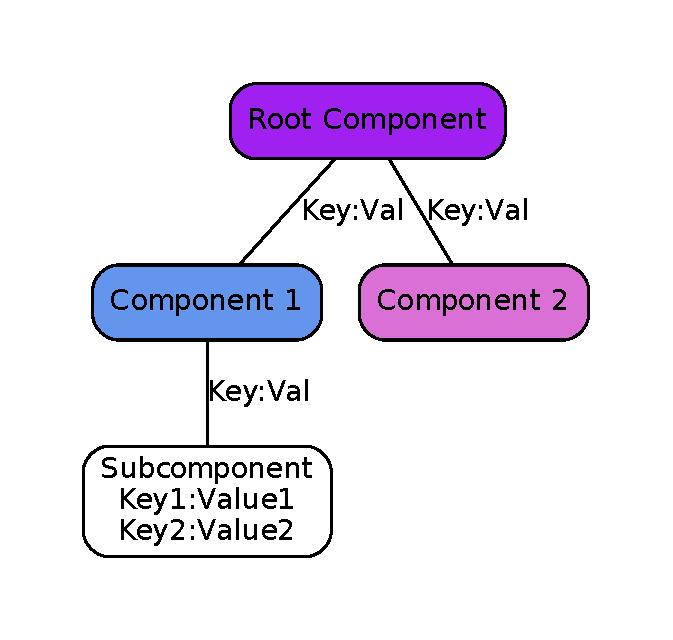
\includegraphics[scale=0.45]{dot/coarse-grained-components}
	\caption{Example of how to specify relationships and characteristics for system components.}
	\label{fig:abstract + key-value}
\end{figure}

The coarse grained model assumes a graph of components -- at this point we do not have to discuss the individual components -- and their relation.
The graph of components is the foundation to compute the resilience, estimate performance and the costs.
An example graph is shown in \Cref{fig:abstract + key-value}.
Component 1 and 2 have dependencies to the root component, and the Subcomponent to Component 1.
Annotations can be placed on edges and nodes; the exact meaning of the figure and the annotations depends on the model.




\newpage
\subsection{Resilience Model}





\begin{figure}
	\centering
	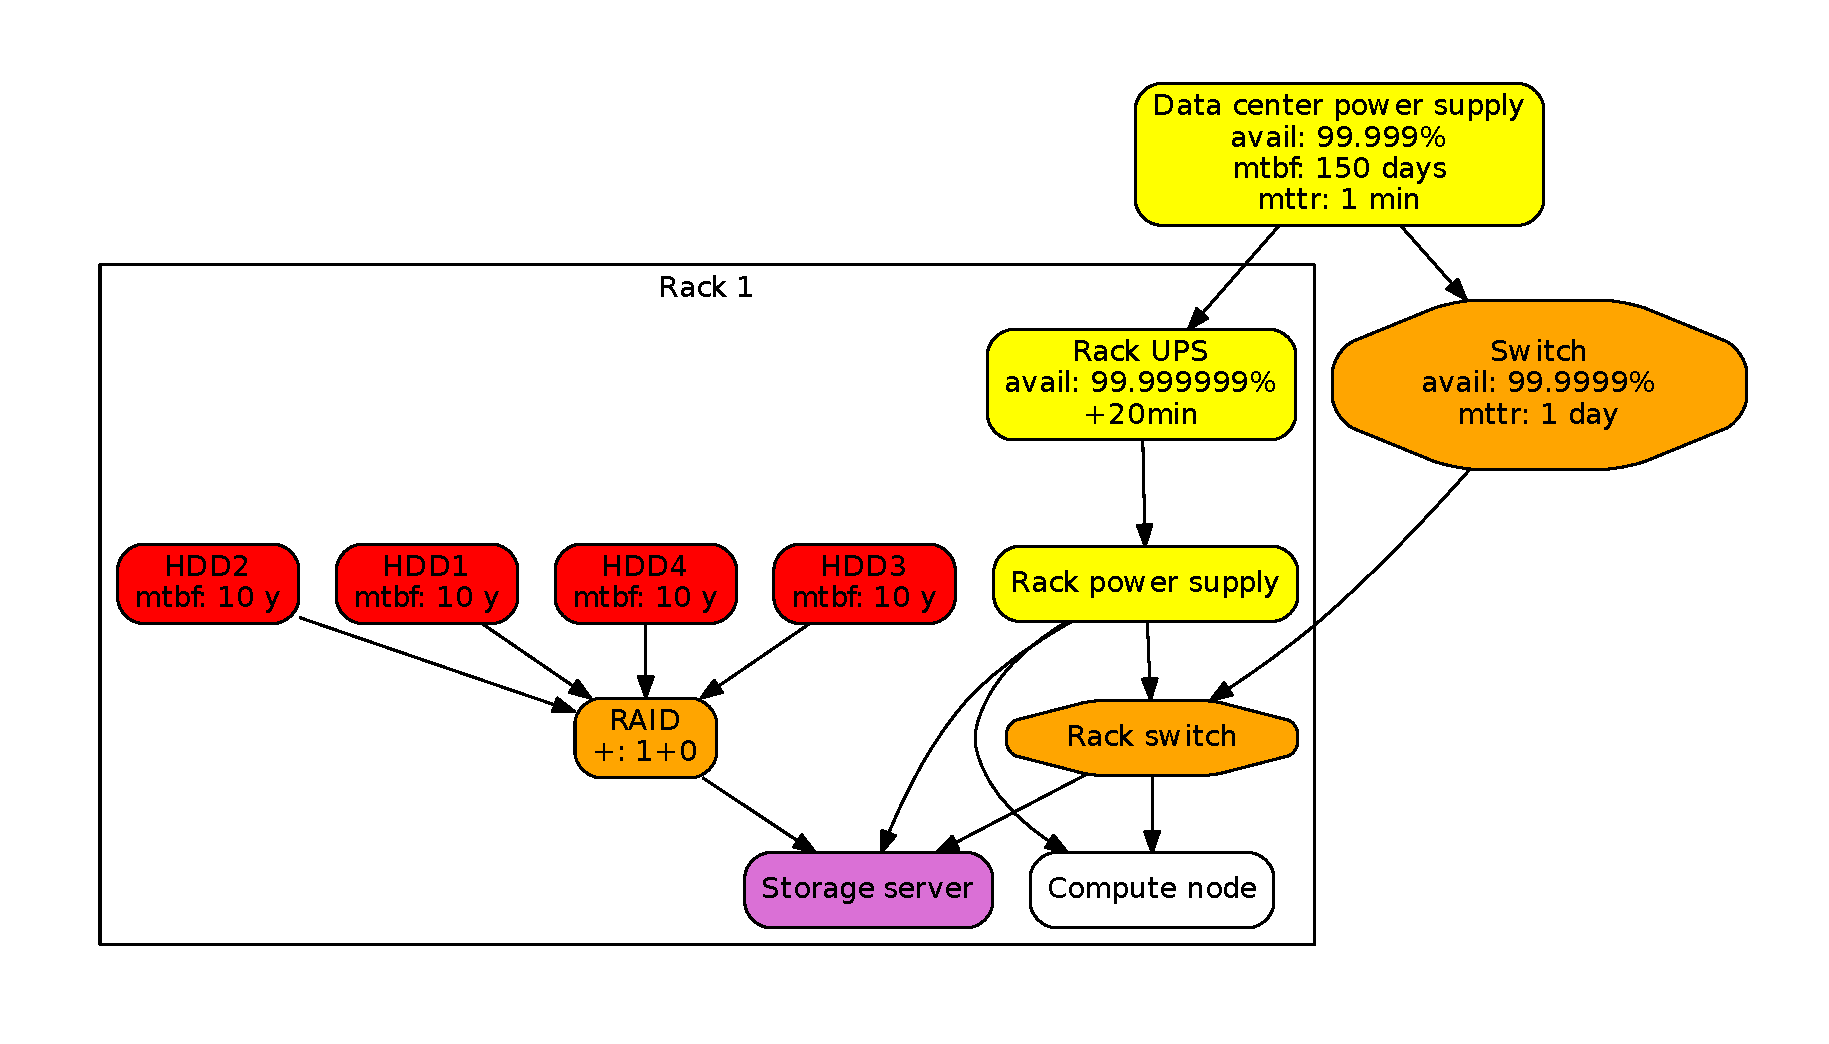
\includegraphics[scale=0.45]{dot/coarse-grained-failure}
	\caption{Component dependency graph to model resilience.}
	\label{fig:resilience example}
\end{figure}


The resilience model is based on component failure metrics and derived using statistical methods.
A very simple example is shown in \Cref{fig:resilience example}.
The graph shows the error propagation of failures, i.e., dependencies of errors, as a directed graph.
For example, if the overall data centre power supply fails, then the global switch fails and the failure is propagated to the Rack UPS (uninterruptible power supply).
However, the UPS actually mitigates this error for an amount of time; still it introduces a new source of error, but if these errors are less likely than a global power outage the overall availability increases.
Thus, such a graph can contain technology and strategies to mitigate errors.
Mitigation strategies usually depend on redundancy, i.e., replication of data, which adds costs and may reduce performance.

Similarly, for block devices, the RAID strategy replicates data and, thus, tolerates failures of individual components.
The annotations in the graph show the MTBF, MTTR, or simply the reliability rate in \% and for mitigation devices some short information.
In fact, for every type of failure, a MTBF and MTTR could be provided to account for different probabilities of the various types of error and the recovery time.

Since mitigation strategies are rather complex, only a short hint is given (after the +).
The level of detail of such a model can be varied, modeling each subcomponents of a node like a CPU, power supply, or memory DIMM.
Or it becomes more coarse grained modeling a data centre on the level of compute, storage, cooling and power supply based on the available data or interest of the modeler.
More coarse grained models can be build usually on the fine (subcomponent based) failure rates.
%\todo{F = failure rate or probability of failure in one hour \url{http://answers.google.com/answers/threadview?id=390140} Define failure and availability rate in definitions!}
%\todo{JJ: Notationally, it would be better to reserve F for the CDF}
To determine the reliability rate of a component, the rate of all components it depends on can be multiplied when modeling independent failures.

\paragraph{Example}
Let us compute the MTBF of the RAID system to fail with RAID 0 and RAID 1+0.  For simplicity, we assume initially a
uniform distribution of errors, i.e., it is equally likely the system fails in the first minute after is has been
started and in one minute after it run 100 days without error.  In other words, if $p$ is the probability of failure in
any given minute, then the assumption is that $p$ is independent of time.

If we look at it discretely, with $\mathbb{T}$ (as a stochastic variable) being the minute a failure occurs (minute 0
being when the device is started), then $\mathbb{T}\sim\mathcal{N}(1,p)$ where $\mathcal{N}(k,p)$ denotes the negative
binomial distribution with parameters $k\in\mathbb{N}$ and $0\leq p\leq 1$.  The expectation is $E(\mathbb{T})=(1-p)/p$.
Returning to the original case, if the MTTF is 10 years\footnote{In practice, the vendor-specified MTTF is more likely
  to be $10^6$ hours or more, which translates to well over 100 years.}, we do indeed get $p=1.9\cdot 10^{-7}$, which is
the probability of failure in any given minute.

In practical reliability engineering, one will often look at the ``bathtub curve'' which includes a component of
``infant mortality,'' i.e.\ early failures of the device which is prominent in the early timespan of the device, as well
as a component of aging which gets prominent obviously in the later stages of the device lifecycle.  On top of that is a
constant probability of failure throughout the lifecycle of the device.  Let us consider these components in turn.

As regards infant mortality, STFC's data centres, for example, will typically ``burn in'' disks by putting them through
high intensity activity for about four weeks, thus ensuring that the early-life device failures get caught before the
drive is put into production.  At the other end of the scale, a drive is typically retired long before its MTTF: if the
MTTF is 10 years, say, the disk server may be retired at 5 or 6, and may even have been reallocated to less critical use
well before then (after 3-4 years), with the critical disk services being taken over by newer disk servers with higher
capacity.  In these cases, one should be able to ignore the sides of the bathtub curve and should get an essentially
constant failure rate.

However, it would likely be a mistake to use the MTTF to derive the constant rate, as the MTTF is based on the aging
device.  We thus need to revisit the data on drive failures.  Moreover, one also needs to take into account the
possibility of systemic failures, like those arising through firmware bugs, environmental disasters (like failure of
cooling or power), or simply the usage which have low likelihood but high impact as they are likely to affect a larger
number of drives.  Also the usage is relevant, where drivers under higher load are more likely to fail, particularly in
the early months of its use \cite{pinheiro}.

%\todo{Statistics here!}

%% \todo{Exponential distributions, reference to work on reliability or survival?
%% JL: If you have particular in mind, drop it here :)
%% }

%The \emph{exponential distribution}, $E(\lambda)$ with parameter $\lambda>0$ is based on the assumption of a constant
%\emph{hazard function}, the constant value being $\lambda$ for $t>0$ -- this means that given that the device has not
%failed at time $t$, the probability of failure in time $t$ to $t+\delta t$ (for small $\delta t$) is $\delta t\lambda$.
%The \emph{survival function} for $E(\lambda)$ is $\exp(-\lambda t)$ for $t>0$.

%\todo{more stuff here, but need the stats first}

%% Even though we are introducing a simple model, we still need to do the maths ``properly,'' otherwise we risk getting the
%% wrong result, and we would need to do the maths properly anyway in order to develop more sophisticated models.  We thus
%% need to introduce a little bit of elementary probability theory.\todo{We could move some of the stuff to appendices}

%% With $p$ as above, time between failures is thus exponentially distributed\footnote{Of course, in practice, once a
%%   device has failed, it is dead; but mathematically, it may make sense to allow failures to recur, a natural consequence
%%   of the independence of time.  In practice, it will not affect the result.} with parameter $\lambda$, which we need to
%% relate to both $p$ and the MTBF.  If $\mathbb{T}$ is the time to fail (as a stochastic variable), then
%% $\mathbb{T}\sim\mathrm{Exp}(\lambda)$.  As the exponential distribution has CDF

%% \begin{equation}
%%   F_{\mathrm{Exp}(\lambda)}(t)=1-e^{-\lambda t},
%% \end{equation}
%% (JJ: TODO - epxand later)

For RAID 0, the RAID system is degraded if any device fails, and again for simplicity we assume failures are independent.
%% This bit is too simplistic, it won't work:
%% Based on the 10 year MTBF, the probability that one device fails in any given minute is $F(HDD) = 1.9\cdot 10^5
%% \%$\todo{this is completely wrong...! (aside from the missing minus), it would be exponential.}
%% The chance that at a given time one of the four HDDs fails is $1 - (1 - F(HDD))^4$ and, thus the RAID system would fail.
%% Based on this value the MTBF of a RAID 0 system can be computed that is 2.5 years.
%% For a RAID 1+0, two HDDs must fail, .... \todo{eintragen}
Instead of using simple models of MTBF and MTTR probability distributions over time could be used.
%\todo{Figure probability distribution of failed HDDs}


\comment{
TODO: more complex model:
* Component failure rate, probability distribution over time, dependencies to other components, graph can show the dependencies (e.g. power failure in a Rack or overheating in a Rack)
* Software must protect against component failures e.g. using erasure coding, redundant components / space.
** RAID / erasure component: RAID0 => x fach replication, ... 1.1 x components needed
=> reduces performance and increases component counts
}

\subsubsection{Performance Model}
\label{sec:modeling:perf}

\begin{figure}
	\centering
	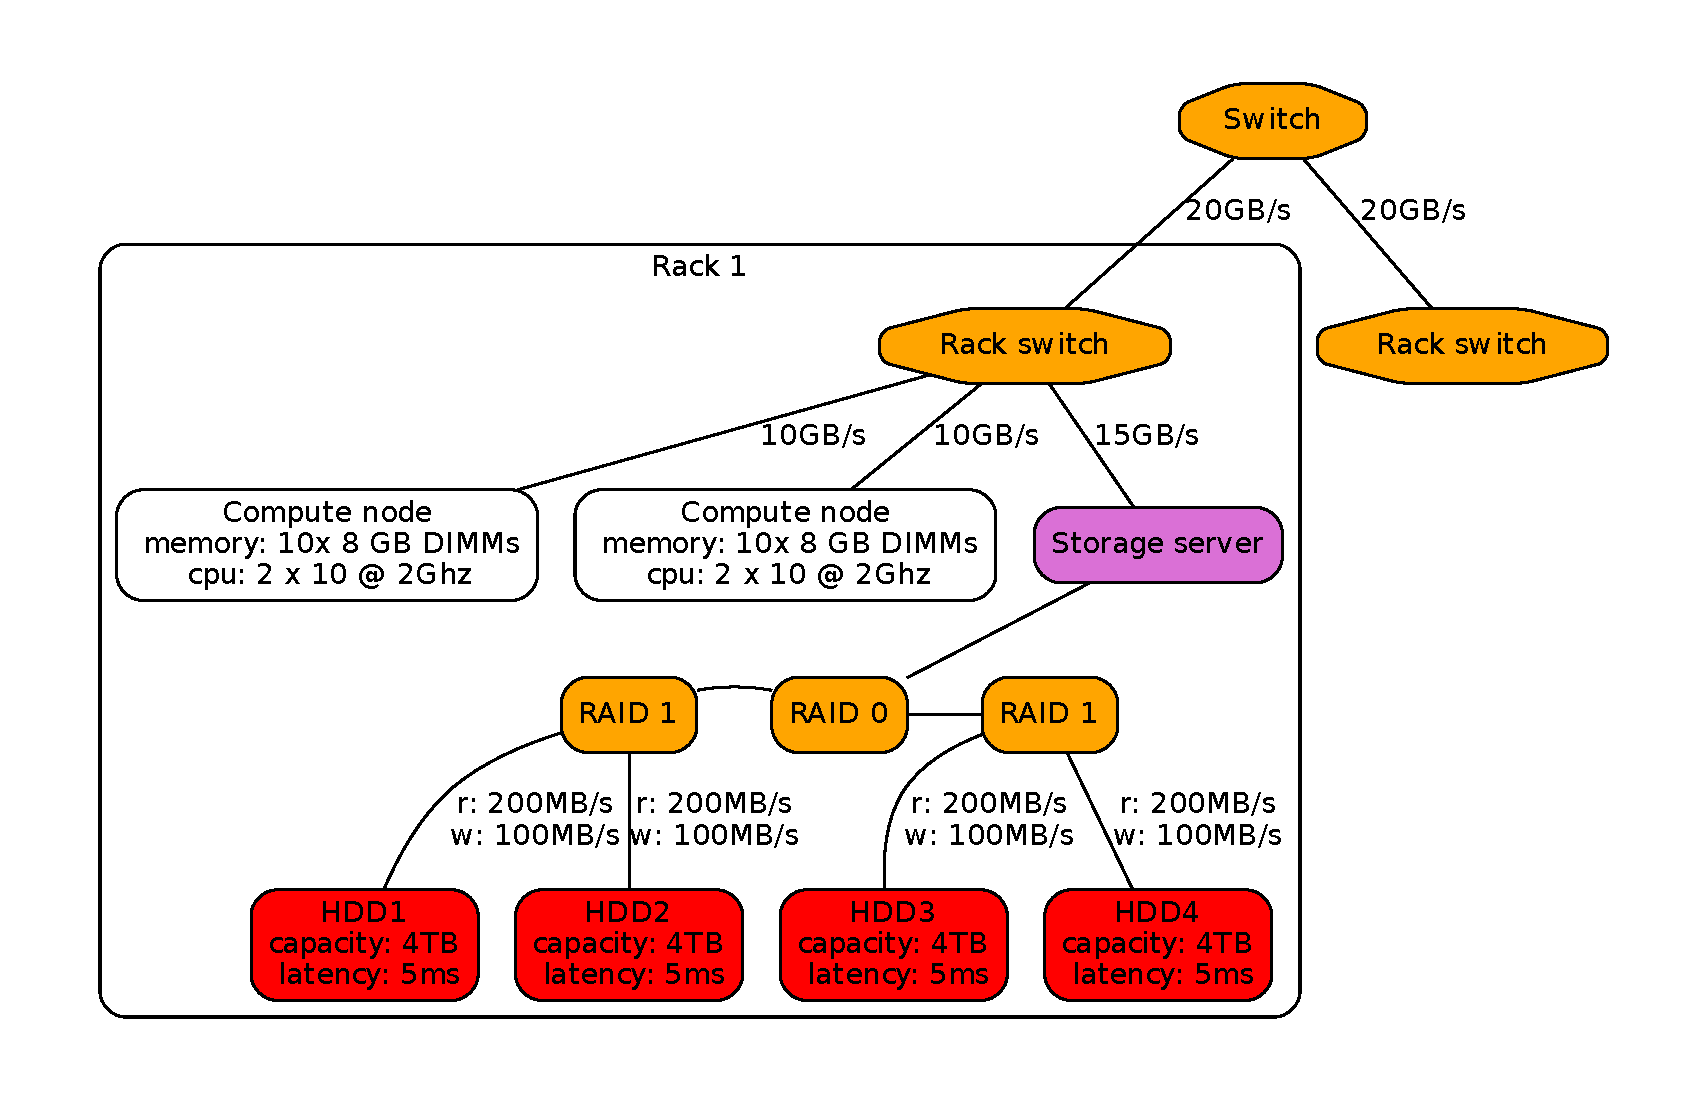
\includegraphics[scale=0.45]{dot/coarse-grained-performance}
	\caption{Component dependency graph to model performance.}
	\label{fig:performance example}
\end{figure}


The performance model also uses a  graph based model annotating relevant components with throughputs and latencies.
Using the hardware graph it is easy to determine theoretic peak performance for individual components.
But also for more complex situations, it is possible to gauge the performance that can be obtained from using components in parallel.

\Cref{fig:performance example} shows an example graph with performance metrics for compute nodes, network and storage media added. E.g. it is simple to see that node to node communication can not exceed bandwidths of 10GB/s, while the storage server will be happy to handle incoming bandwidths of up to 15GB/s.
While networks are relatively simple, storage media require a more granular approach to account for different transfer rates for read or writes.
The throughput for paths to the network is simply defined by $max(edge0_{throughput}, ..., edgeN_{throughput})$.
Similarly the latency is the accumulation of latencies attached edges and nodes on the path $\sum_{item}^{path}{item_{latency}}$.

For common groups of components used in combination such as RAID systems it can be useful to not model the complexity explicitly as the dynamics are sometimes well understood can be abstracted as described in \cite{kunkel_iopmmodeling_2012}.
For example for a deployed RAID 1+0 the relevant performance of interest is no longer the performance of the individual HDDs but the performance of the RAID group.
This can be derived in two steps:

\begin{enumerate}
	\item RAID1 has performance implications in two most notable ways: the throughput is slightly reduced and capacity is reduced.

\begin{align}
	 & RAID1_{capacity}   &  & = min(child0_{capacity}, ..., childN_{capacity})     \\
	 & RAID1_{throughput} &  & = min(child0_{throughput}, ..., childN_{throughput}) \\
	 & RAID1_{latency}    &  & = max(child0_{latency}, ..., childN_{latency})
\end{align}


	\item RAID0 pushes in the opposite direction. Throughput and capacity can be obtained by taking the sum of the direct children:
\begin{align}
	 & RAID0_{capacity}   &  & = \sum^{children}{child_i:capacity}   \\
	 & RAID0_{throughput} &  & = \sum^{children}{child_i:throughput}
\end{align}
\end{enumerate}



%\url{wr-publications/Papers/2012/kunkel-pdp12-abstraction_and_graphical_modeling}

%* annotated graph of the components, how data flows, costs for additional software stacks / middleware
%* throughput model parallelism from n clients / aggregated across all clients







%\subsubsection{Workload Model}
%
%A coarse grained workload model defines the required performance characteristics for the executed workload mix.
%Naturally, some components must be sized based on the most intense workload run on this component.
%For example, the memory capacity of a node must be sized to meet the needs for the memory occupied by the biggest application -- in this specific example otherwise more nodes would be needed and available resources would be wasted.
%
%Example for the execution of a specific application (fine grained).
%Beispieltrace wie eine Anwendung laufen könnte in verschiedene Phasen.
%Das kann resultieren in aggregierten Leistungsdaten wie Cite aus paper.
%
%We assume performance characteristics for the data centre have been derived from the workloads.
%Note that this is similar to the typical estimation strategy used during the procurement of new HPC systems.


\subsection{Cost Model}

%
%\begin{figure}
%	\centering
%	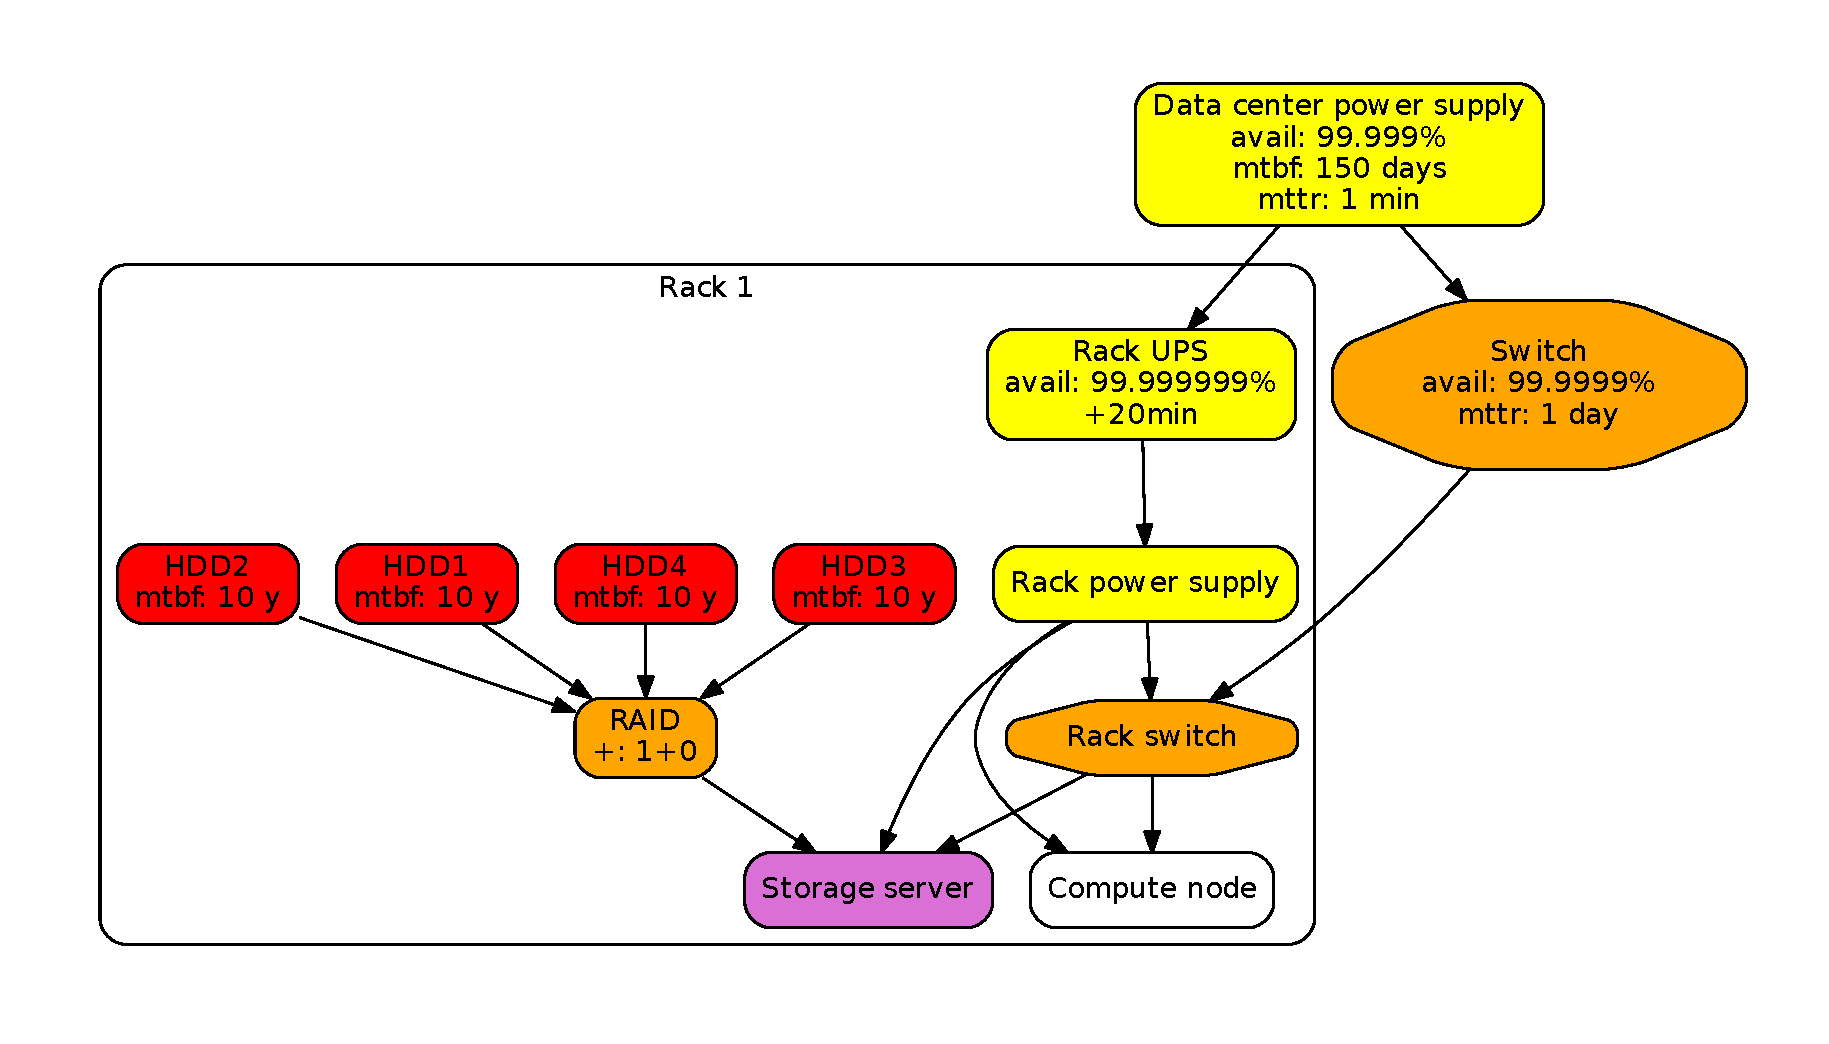
\includegraphics[scale=0.49]{dot/coarse-grained-cost}
%	\caption{Component dependency graph to model cost.}
%	\label{fig:}
%\end{figure}

The cost model can be divided into a model for operating a supercomputer and the costs for executing a scientific workflow.

\paragraph{Supercomputer TCO}

The total costs of ownership for a system depends on the investment costs and the operational costs.
\Cref{eq:tco} gives an idea how the TCO can be computed based on individual components.


\begin{align}
\label{eq:tco}
TCO(system)  & = \mbox{investment costs} + \mbox{operational costs} \nonumber \\
\mbox{investment costs} & = \mbox{costs for hardware components} + \mbox{support contract} \\
\mbox{operational costs} & = \mbox{facility} + \mbox{staff} + \mbox{maintenance} + \mbox{energy} \nonumber
\end{align}

In the equation it is assumed the operational costs are accumulated over the lifetime\footnote{The time a system or component is in production.} of the system.
Potentially, the investment costs could contain already the costs for the support during the system's lifetime -- this is typical for procurements of public data centres.
Other cost factors are usually integrated into one of these factors, for example, cooling costs are integrated in the energy costs and the cooling hardware infrastructure in the facility costs (for the lifetime of a system).

Many of the listed costs can be easily distributed across the individual components of the system.
For example, the investment costs for a system is the sum of the costs for the individual components (and some extra costs for planning and integration).
However, in some cases the distribution of costs across subcomponents is not trivial:
When hosting multiple systems into one building, one issue is how to divide fixed operational costs like facility and staff costs across IT equipment?
Facility costs could be distributed based on the percentage of occupied floor space.
Staff could be employed for a dedicated system but is usually shared for all systems making it difficult to account for.
A typical assumption could be that a fixed number of staff people is needed regardless of the number of components in the system due to the economy of scale.

%\todo{Componenten graph mit Kosten?}
\comment{
Mitigation strategies usually depend on redundancy, i.e., replication of hardware, this adds costs.
Dependency graph of costs.
for a fixed configuration:
* count components

Bei veränderung der Komponentenanzahl, ein Lineares Modell, in realität gibt es nichtlineare Sprünge, bspw. wenn der Switch nicht mehr aussreicht für alle kabel.
}



\paragraph{Costs for executing scientific workflows}

The costs for some workload W depends on its usage behavior on all stressed components of the system.
The usage of exclusively used resources implies costs based on the fraction of used resources divided by the overall available resources.
For example, if 10\% of a system is used for 100\% of its lifetime, this should cost about 10\% of the TCO for the system.


A naive approach of computing the costs for the workload is given in \Cref{eq:distributeCosts}:
\begin{align}
\label{eq:distributeCosts}
\mbox{costs}(W) = \sum_{\mbox{c}} \frac{\mbox{TCO(c})}{\mbox{lifetime(c)} \cdot \mbox{resources(c)}} \cdot \gamma(c)  \cdot \int_{t = 0}^{T} {\mbox{u}(W,c,t)}
\end{align}
By dividing the TCO for each component that is used with its lifetime and amount of resources it offers, the relative costs per second and resource utilized is computed.
This value then has to be multiplied with the actually utilized resources over time.
$u(W,c,t)$ are the used resources at a given time for the workload W and this component.

However, overall the system might experience periods in which it is idle.
Thus, as these times also incur costs but cannot be assigned to a workload, they must be assigned to actual workloads.
The utilization of a component can be defined as the fraction in its lifetime it is doing useful work, e.g., typical supercomputers are scheduling production jobs in more than 90\% of their lifetime.
Since the final utilization is not known a-priori and would require to determine the actual usage of the component until the end of its lifetime, an empiric estimate can be used.
To accommodate for unused resources, the costs for a job can be multiplied with the inverse of the estimated utilization of the component to account these costs to the job.
$\gamma$ as inverse of the utilization is our correction term $> 1$, e.g., with a value of 1.1 for compute node utilization.









There are costs which depend on the actual usage behavior, e.g., the consumed energy and, thus, energy costs, are influenced by the behavior of the workload.
For simplicity, we will not consider them explicitly in our coarse grained model.

Note that this model can be applied to many resources, as for example, jobs running on compute nodes.
Also, costs caused by passive behavior such as files occupying on a storage system imply costs in a similar fashion.
As costs of idle data can be significant, we describe a model for them explicitly and demonstrate the overall concept on this example.

\paragraph{Costs for idle data}

To quantify the costs for idle data, we recapitulate the life cycle of data first\footnote{Please also see the paper \cite{CECOSDKMKL10} that describes how this information could be gathered and how energy consumption could be computed.}.
See \Cref{fig:datalifecycle} for an example of a file's life cycle.
In the example, we assume a simulation which iteratively updates the current state and stores the computed results in a file -- that is, appends them.
It consists of different phases (file creation, running of the simulation), post-processing, later analysis by other scientists and deletion.
A vertical bar indicates a discrete time which triggers I/O activity during a particular phase.
The modifications to the file size are shown in \Cref{fig:size_changes}.
A post-processing (or visualization of the results) requires to read the data and might generate derived results.
Later, additional analysis might be conducted with the simulated data.
For instance, to compare the old results with newer results or to answer new scientific questions with the recorded simulation results.
Over time, data loses its importance and is accessed less often -- gradually losing value in terms of the need for fast access -- and ultimately gets archived (moved to a slower less expensive medium, such as on-line, near-line, or off-line tape) or disposed of.
As a rule, newer data and data that must be accessed more frequently is stored on faster but more expensive storage media, while less critical data is stored on cheaper but slower media.
However, the actual usage of data depends on the use case and on the user interaction.

\begin{figure}
\centering
  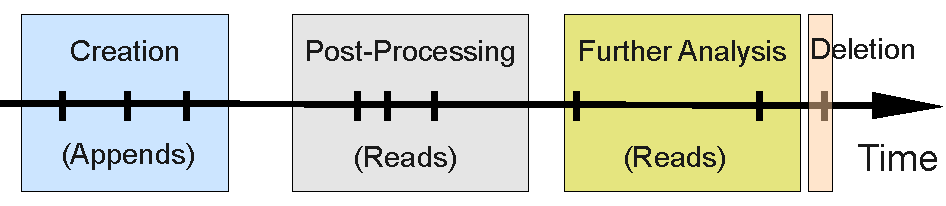
\includegraphics[width=.45\textwidth]{figures/old-papers/life-cycle}
\caption{Example scientific data life cycle}
\label{fig:datalifecycle}
\end{figure}


\begin{figure}
\centering
  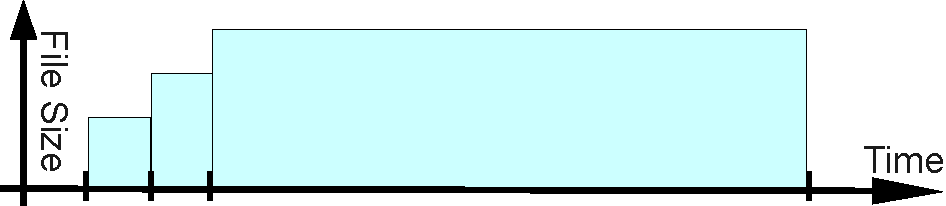
\includegraphics[width=.45\textwidth]{figures/old-papers/size_changes}
\caption{Trivial file size increases during the life cycle}
\label{fig:size_changes}
\end{figure}


The costs for storing a file on the system could be computed by understanding the space occupied on the available storage system over time.
In that sense, it can be computed analogous to the costs of an workflow in \Cref{eq:distributeCosts}.
That means, a file that occupies 10\% of space for the whole production time of a storage system should be budgeted with 10\% of the costs for supporting the storage system for its lifetime, i.e., its TCO.
Similarly, a file that occupies 20\% of space for half the production time is also budgeted with 10\% of the storage system's TCO.
For a file, the integral of the occupied space, that means, the file size over time is the relevant metrics to compute the fraction of costs from the TCO that it accounts for.
Thus far this model does not account for the costs of empty space (which might be necessary for performance reasons, or which might be a consequence of an initially empty resource filling up), but this can be dealt with by identifying $\gamma$  to be a ``fill factor'' which might vary between something like $1.05$ to represent $5\%$ ``performance headroom'' and $1.5$ for an initially empty resource which is filled by the end of the lifetime of the resource.

Based on these considerations an equation can be constructed:
\begin{align}
%\caption{Computing costs for idle files}
\label{eq:idlefiles}
\mbox{costs-idle}(F) = \frac{\mbox{TCO}}{\mbox{lifetime} \cdot \mbox{capacity}}  \cdot \gamma \cdot \int_{t = 0}^{T} {\mbox{size}(F,t)}
\end{align}

\Cref{eq:idlefiles} computes the (idle) costs for keeping a file on the storage.
$F$ is the file, $t$ the discretized time.
$\mbox{size}(F,t)$ is the size the file occupies at a given time.
Capacity, lifetime and TCO refer to the storage system's total capacity, the lifetime and TCO, respectively.
$\gamma$ is the ``fill factor'' correction term $> 1$, e.g., 1.1, to accommodate for empty space.

Theoretically, the costs for transferring data (i.e., for active files) could be captured by measuring the amount of data accessed and number of I/O operations.

\paragraph{Example}
To demonstrate how a HSM system which consists of spinning disks and tape could migrate data, a simple scenario is setup.
Consider an iterative application which appends 10\,G\-Bytes of data to a file every 10 minutes.
For instance the application could be a climate simulation which runs for 1,000 minutes, that is, performs 100 iterations.
In total a single file of 1\,TByte is created.
After completion of the program, in a post-processing phase, data is extracted, post-processed and 100 minutes later the whole data set is visualized -- that is, data is read completely two times.
Then -- at the end of the post-processing phase -- the data is migrated to tape.

\begin{figure} [htb]
\centering
  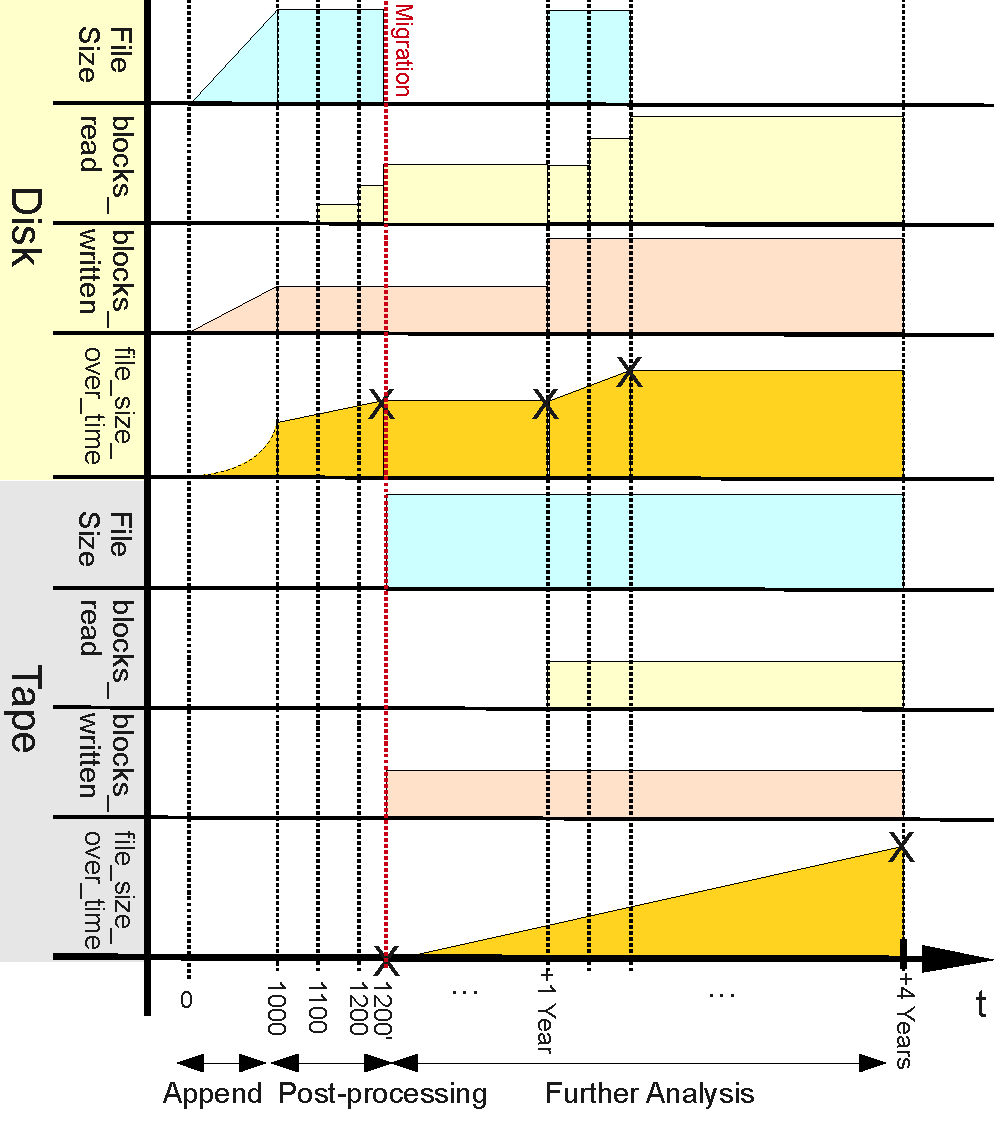
\includegraphics[width=.75\textwidth]{figures/old-papers/example-ea}
\caption{A qualitative view of the contributions to the terms of equation \ref{eq:idlefiles} for the example scenario with migration between tape and disk (note that
the \texttt{file\_size\_over\_time} terms correspond to the integral term in that equation). }
\label{fig:exampleEA}
\end{figure}

In a phase of further analysis the data is requested one year later to perform new analysis and compare the simulation run with new data.
Between each run 100 minutes elapse.
Therefore, data is staged from tape to disk and read sequentially two times by various applications.
Then the data on disk is deleted immediately.
The changes of various metrics such as file size on the device, blocks read, and the integrated file size are shown in \Cref{fig:exampleEA}.

In this example one could use use equation \ref{eq:idlefiles} to sum up the costs of the storage on disk in each phase, and the cost of the tape.
A key confounding problem in this sort of analysis is whether or not the data recall from tape requires recall of more data because of packaging considerations (\Cref{sec:packaging_and_metadata}).


%%%%%%%%%%%%%%%%%%%%%%%%%%%%%%%%%%%%%%%%%%%%%%%%%%%%%%%%%%%%%%%%%%%%%%%%%%%%%%%

\section{Modeled Components}
\label{sec:modeling/components}

The previous section covered the bigger picture of the approach. This section serves as reference for considerations that apply to common subsystems and components.
In some cases more detailed models are required in support of the course grained models this section collects abstract cost and performance information for various components and subsystems relevant to storage systems in data centres.
\Cref{sec:modeling/components/unconfigurable} collects individual components that are usually not configurable.
The implications by key configuration choices for compute nodes and I/O nodes are listed in \Cref{sec:modeling/components/computenodes} and \Cref{sec:modeling/components/ionodes} respectively.
\Cref{sec:modeling/subsystems} discusses similar considerations for important storage subsystems such as object stores, parallel file systems or tape systems.


%%%%%%%%%%%%%%%%%%%%%%%%%%%%%%%%%%%%%%%%%%%%%%%%%%%%%%%%%%%%%%%%%%%%%%%%%%%%%%%
\subsection{Unconfigurable Components}
\label{sec:modeling/components/unconfigurable}

Many components in data centres cannot be internally configured and have to be purchased as unit components or appliances. However, it is still important to consider these units as their characteristics determine e.g. peak performance and cost of higher level components and subsystems.

\begin{itemize}
	\item Processing Units: CPUs, Accelerators, possibly FPGAs
	\item Memory: DIMMs
	\item Storage: HDDs, SDDs, Tapes
	\item Other: NICs, PCI Cards
\end{itemize}

Each of the components is associated with performance values in regard to:

\begin{itemize}
	\item Unit Price, Throughput (read, write), Capacity, Power Consumption
\end{itemize}


%%%%%%%%%%%%%%%%%%%%%%%%%%%%%%%%%%%%%%%%%%%%%%%%%%%%%%%%%%%%%%%%%%%%%%%%%%%%%%%
\subsection{Compute Nodes}
\label{sec:modeling/components/computenodes}

%\begin{figure}
%	\centering
%	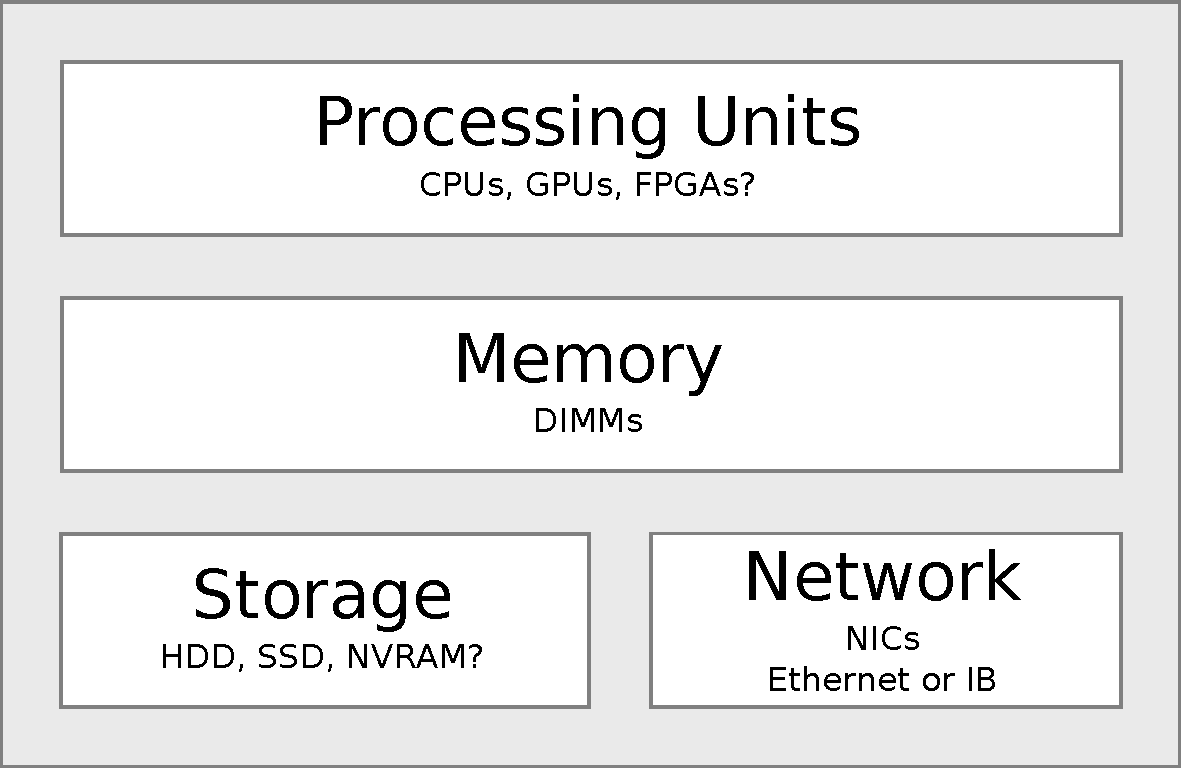
\includegraphics[width=0.5\linewidth]{figures/components_compute-node.eps}
%	\caption{A typical compute node.}
%	\label{fig:componentscompute-node}
%\end{figure}


\begin{figure} [htb]
	\centering
	\begin{subfigure}[t]{0.49\textwidth}
		\centering
		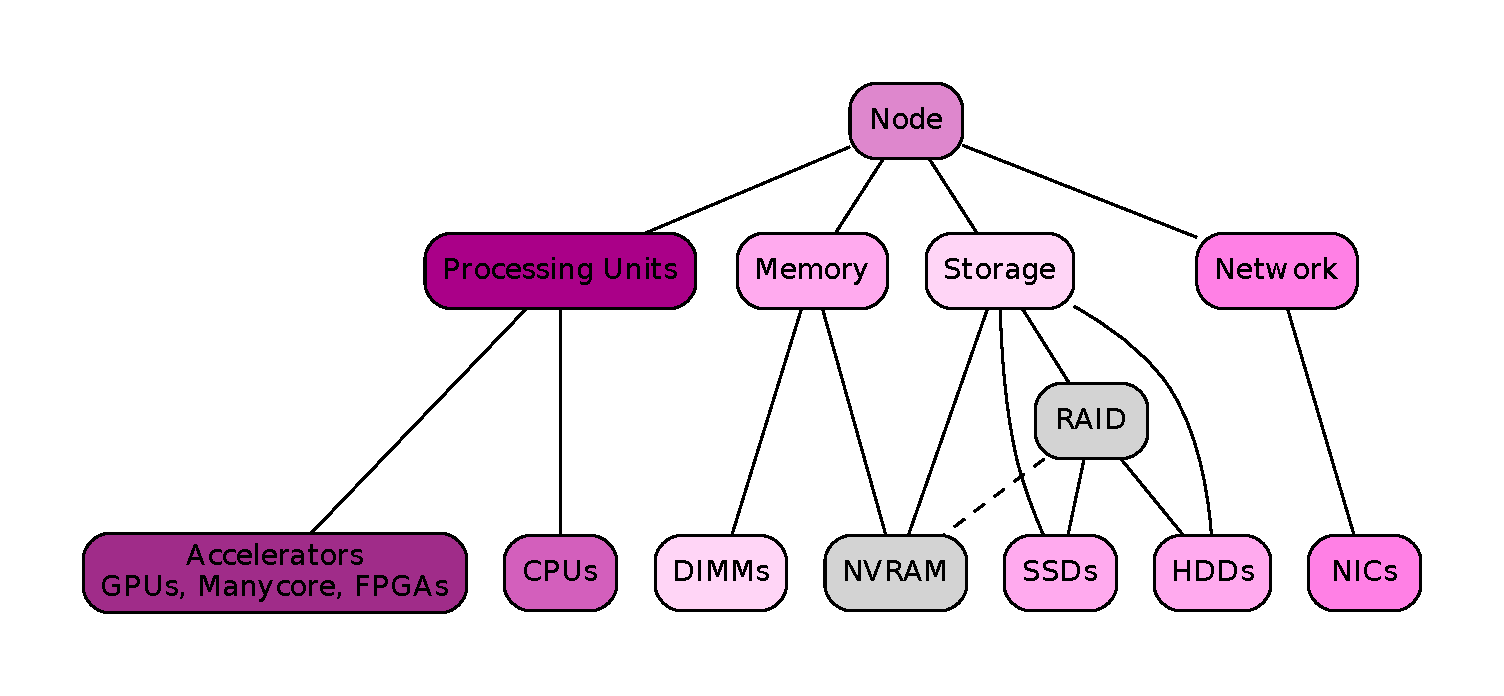
\includegraphics[width=\textwidth]{dot/model_node_cost/compute_cost}
		\caption{cost}
	\end{subfigure}
	\begin{subfigure}[t]{0.49\textwidth}
		\centering
		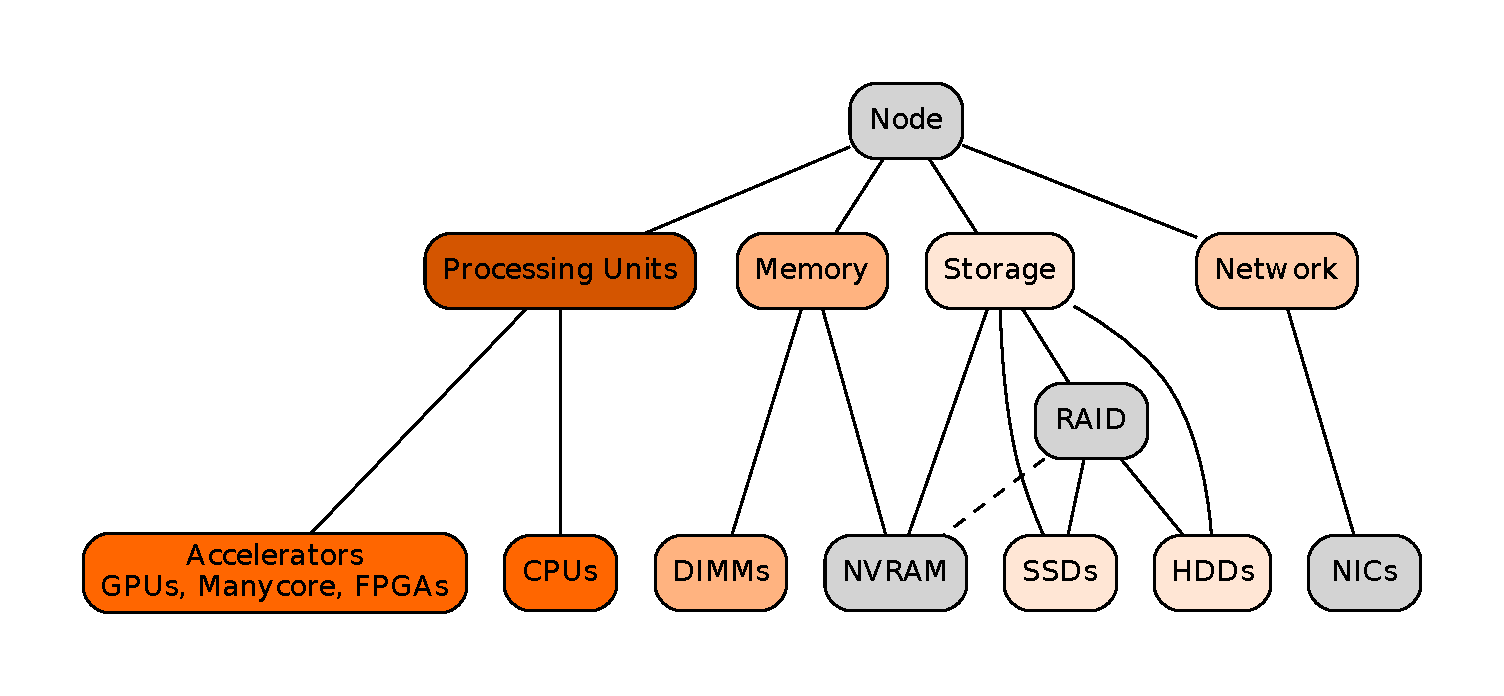
\includegraphics[width=\textwidth]{dot/model_node_cost/compute_power}
		\caption{power}
	\end{subfigure}
	\caption{Cost and power footprint bay component for compute nodes. A darker shade represents a larger share relative to the total node configurations.}
	\label{fig:components-compute-node}
\end{figure}

Compute nodes come in various flavours.
Depending on the task different configurations are useful.
For climate simulations for example, nodes usually require substantial amount of compute power and memory in combination with a low latency network.
%Other use cases such as visualization or increasingly big data workloads, maybe less dependent on synchronous communication.

\paragraph{Storage related factors for compute nodes:}
\begin{itemize}
	\item  CPU / GPU / Processors:
	\begin{itemize}
		\item How fast can be data processed or generated?
		\item Is there spare processing power e.g. that can be invested into data reduction or more intelligent data handling?
	\end{itemize}

	\item Memory
	\begin{itemize}
		\item Affects the problem size that can be held quickly accessible on the node.
		\item Can greatly improve storage performance by use of caching.
		\item Maybe contended by e.g. network components that require buffers.
	\end{itemize}

	\item Storage (Node Local)
	\begin{itemize}
		\item Usually too slow for large amounts of data in comparison to PFS/Object Storage.
		\item How will this change as node local NVRAM and burst buffers become more affordable?
	\end{itemize}

	\item Network Adapters
	\begin{itemize}
		\item Determines how fast nodes may communicate with each other.
		\item Determines how fast we can drain data away from the compute nodes e.g. when writing snapshots.
		\item Determines how quickly compute can begin.
	\end{itemize}

\end{itemize}

%%%%%%%%%%%%%%%%%%%%%%%%%%%%%%%%%%%%%%%%%%%%%%%%%%%%%%%%%%%%%%%%%%%%%%%%%%%%%%%

\subsection{I/O Nodes}
\label{sec:modeling/components/ionodes}


%\begin{figure}
%	\centering
%	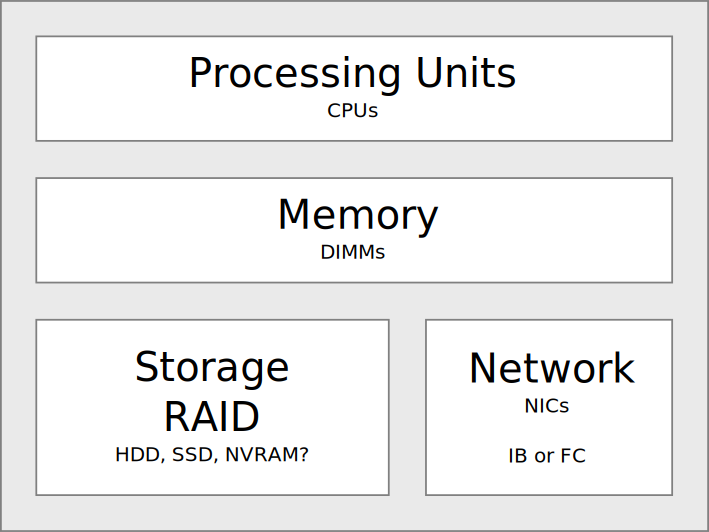
\includegraphics[width=0.5\linewidth]{figures/components_io-node.eps}
%	\caption{A typical I/O node.}
%	\label{fig:componentscompute-node}
%\end{figure}


\begin{figure} [htb]
	\centering
	\begin{subfigure}[t]{0.49\textwidth}
		\centering
		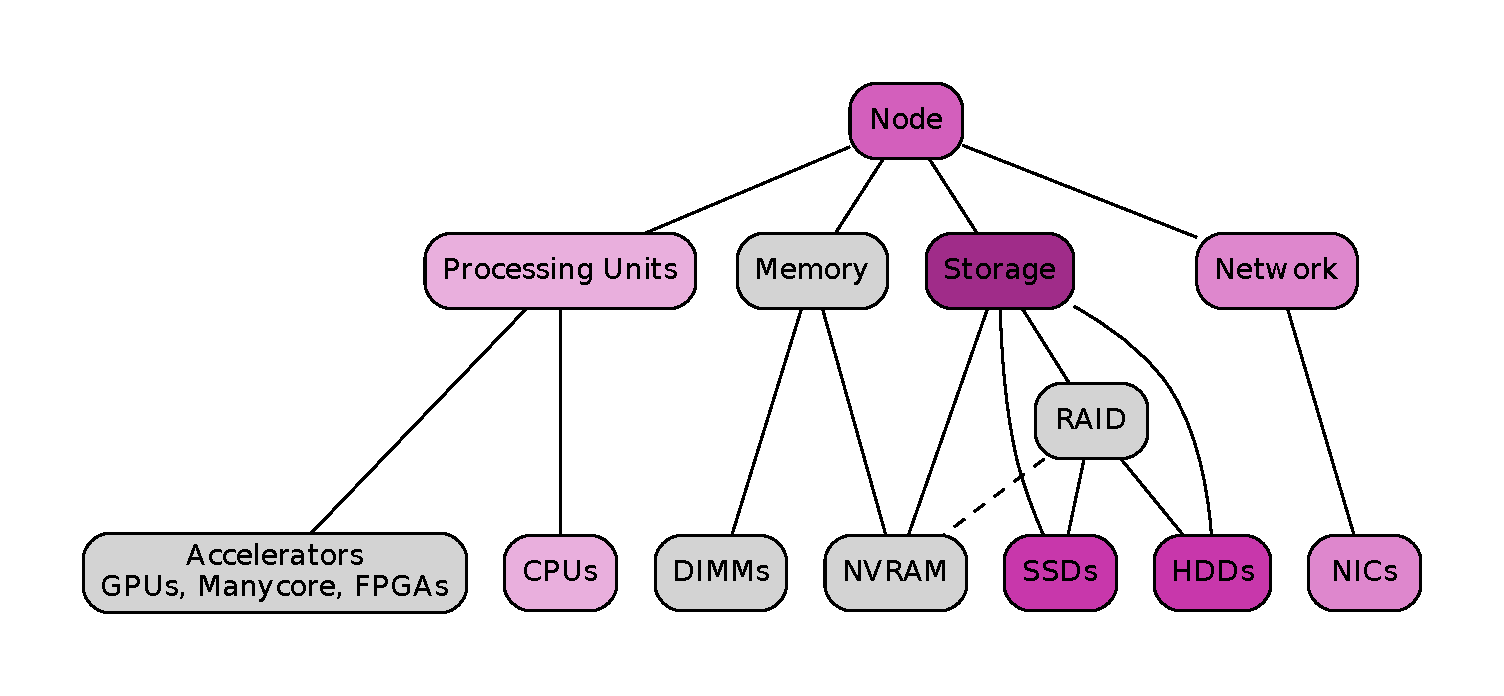
\includegraphics[width=\textwidth]{dot/model_node_cost/io_cost}
		\caption{cost}
	\end{subfigure}
	\begin{subfigure}[t]{0.49\textwidth}
		\centering
		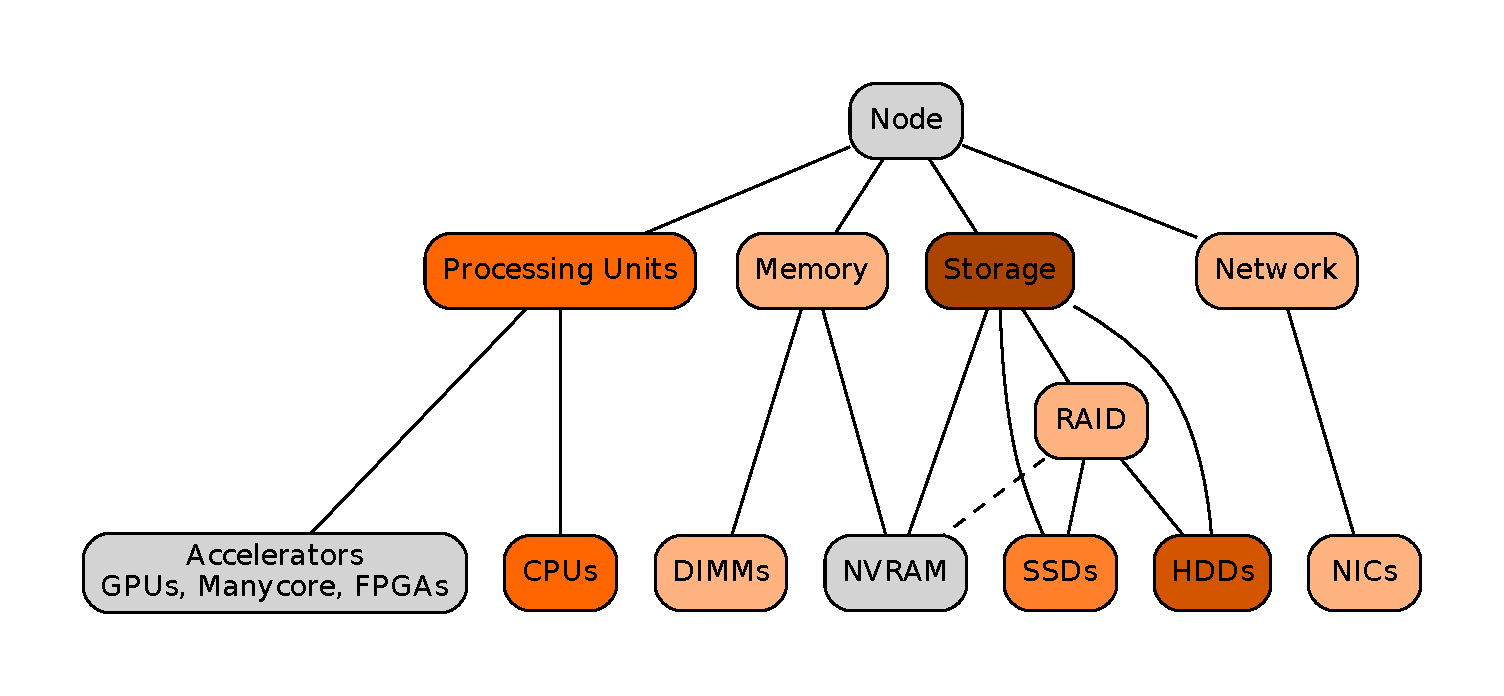
\includegraphics[width=\textwidth]{dot/model_node_cost/io_power}
		\caption{power}
	\end{subfigure}


	\caption{Cost and power footprint bay component for I/O nodes. A darker shade represents a larger share relative to the total node configurations.}
\label{fig:components-compute-ionode}
\end{figure}


I/O nodes are used by all parallel file systems. I/O nodes are specialised nodes with the only purpose to handle requests that the storage subsystem receives. At the same time I/O serve as an intermediate cache layer. Different type of I/O nodes are common:

\paragraph{Load Balancers:}
Either special switches, or more or less compute only nodes responsible to assign targets for read and write access.
In general this is probably not a cost factor for deployments with no need to strictly separate customers.

\paragraph{Metadata Handlers and Targets:}
Especially file systems use metadata targets with configurations optimised for high IOPs and mostly small reads and writes. (Metadata servers can
often be configured with very different storage media than the data handlers they serve, in particular, they often have faster and more expensive
solid state disks, and may be candidates for SCM.) The number of meta data handlers and targets is proportional to the amount of objects that need to stored.
% Bryan guessed what the half complete sentence was meant to say.

\paragraph{Data Handlers and Targets:}
Data targets are configured for capacity and high throughput.
Data targets may feature quite a bit of memory for caching but the cost is dominated by the amount of hard drives.
For HPC systems usually larger reads and writes are observed, for data base systems also the data targets might profit substantially from the usage of SSDs
RAID controllers may also be a factor but software based RAID is becoming very popular for being more flexible.

\paragraph{Factors by component:}
\begin{itemize}
	\item  CPU / GPU / Processors:
	\begin{itemize}
		\item How many requests can be handled by a single node?
		\item Is there spare processing power e.g. for data reduction and other in-transit transformations?
	\end{itemize}

	\item Memory -  e.g. as a quick cache layer.

	\item Storage in RAID
	\begin{itemize}
		\item Storage media is bundled into RAID for performance and fault tolerance.
	\end{itemize}

	\item Network Adapters
	\begin{itemize}
		\item Commonly these nodes use a expensive interconnect.
		\item Determines how fast nodes may communicate with each other.
		\item Determines how fast we can drain data away from the compute nodes e.g. when writing snapshots.
		\item Determines how quickly compute can begin.
	\end{itemize}

\end{itemize}





%\paragraph{Cost driving factors}
%
%\begin{itemize}
%	\item Meta Data Handlers and Targets
%		\begin{itemize}
%		\item Main memory for caches in handlers
%		\item SSDs in targets
%	\end{itemize}
%
%
%	\item Data Handlers and Targets
%		\begin{itemize}
%		\item Storage media (mostly disk count)
%		\item RAID controllers when hardware RAID is used
%	\end{itemize}
%\end{itemize}



%%%%%%%%%%%%%%%%%%%%%%%%%%%%%%%%%%%%%%%%%%%%%%%%%%%%%%%%%%%%%%%%%%%%%%%%%%%%%%%

\section{Data Centre subsystems}
\label{sec:modeling/subsystems}

In this section we discuss other sub-systems which are built up from components, but given the bespoke complexity typical of any application, we do not provide any further diagrams in this section - although we will produce such diagrams in planned future work looking at comparisons of data centres.

%%%%%%%%%%%%%%%%%%%%%%%%%%%%%%%%%%%%%%%%%%%%%%%%%%%%%%%%%%%%%%%%%%%%%%%%%%%%%%%
\subsection{Network: Switches and Interconnect}


The cost of an interconnect network is usually dominated by the number and length of the requisite network cables which in turn depends main on the chosen topology (but also on the physical layout of the data centre\footnote{For example, shorter network cables might be possible if the topology allows compute to be interspersed with storage, and the situation is likely to be further complicated by the advent of hyper-converged compute and storage systems.}).

The secondary cost driver in most networks is the number, type and size of switches, which again is topology dependent.

Some popular network topologies in primarily compute data centres are:

\begin{itemize}
	\item Fat Tree, high bisection bandwidth at reasonable costs. Connections closer to the root switch have higher bandwidth.
	\item 3D Torus, well suited to represent the spatial properties of physical simulations.
	\item Hybercube. Also in form of incomplete hypercubes with similar properties at a fraction of the cost. Good performance and resilient to node failures.  % https://en.wikipedia.org/wiki/Hypercube
\end{itemize}

In general, variations of fat-tree are used for storage only network interconnects, however, in many weather and climate data centres, storage networks share the compute interconnect - whatever that is. The actual network technology is also a significant factor on both cost and performance, with several options available, although Ethernet and Infiniband  (both offering a range of possible bandwidths) dominate, particularly for parallel file systems.  FibreChannel is not often used, and Intel's new OmniPath is now a consideration.

\paragraph{Factors by component:}
\begin{itemize}
	\item  CPU
	\begin{itemize}
		\item Is the network completely offloaded from the CPU?
		\item Cost and bandwidth of network cards will vary by network type (and bandwidth).
	\end{itemize}

	\item Memory
	\begin{itemize}
		\item  Maybe contended by e.g. network components that require buffers.
	\end{itemize}

	\item Network Adapters
	\begin{itemize}
		\item Usually specialised chips by network vendors. Often not software defined, which can lead to the necessity for multiple network adaptors
		(e.g. to support I/O and compute interconnect independently).
		\item May use different speed interconnects in different parts of the network topology (e.g. 10 Gbit to data processing clients and 100 Gbit to data processing servers, similarly, high bandwidth interconnects between switches, lower bandwidth to clients.)
		\item In HPC not uncommon to find only high-performance network.
	\end{itemize}

\end{itemize}


%\todo{are switches energy hungry in comparison?}

\paragraph{Cost driving factors}
\begin{itemize}
	\item Choice of topology, both within and between sub-systems.
	\begin{itemize}
		\item Number of connections/cables.
		\item Length of cables
		\item The number of switches and other network supporting hardware.
	\end{itemize}
\end{itemize}


%%%%%%%%%%%%%%%%%%%%%%%%%%%%%%%%%%%%%%%%%%%%%%%%%%%%%%%%%%%%%%%%%%%%%%%%%%%%%%%

\subsection{Parallel File Systems}

Most of the storage workload on most HPC systems is handled using parallel file systems which expose a POSIX\footnote{The storage interface part of the portable operating system interface, POSIX, exposes a range of I/O interfaces.}) interface. Data is arranged on partitions which provide directories and files organised in a nested tree-like structure, with significant associated metadata including access control criteria, timestamps of last-access etc.

Files are generally spread across multiple storage targets, and so data access requires considerable interactions with metadata, and in particular, data writes involve locking of resources on multiple nodes.  On massively parallel environments these file systems often need to be partitioned inflexibly into pools for reliability or performance isolation and are expensive. Given performance issues around bottlenecks for the metadata operations as well, other storage options are being investigated, and likely to be deployed - which is one of the motivations for cost and performance modelling within ESIWACE. However, even were parallel file systems are baed on open-source software (such as lustre), they are  often procured as appliance units because otherwise it would be difficult to address (or get vendors to own) performance issues --- which can arise in the hardware, software, or the combination of both.

\paragraph{How to estimate cost and performance?}
\begin{itemize}
	\item Cost: Disks, number of disks per storage server, number of storage servers, internal networking.
	\item Performance: Size and type of media, network used, number of storage and metadata servers, amount of RAID required, pool configuration. Note that the aggregate performance will differ from the maximum single-client performance, and both will need to be known (and potentially differ within a single system if different sized pools are used with different user or system defined striping configurations).
\end{itemize}



%%%%%%%%%%%%%%%%%%%%%%%%%%%%%%%%%%%%%%%%%%%%%%%%%%%%%%%%%%%%%%%%%%%%%%%%%%%%%%%
\subsection{Object Storage}

File systems generally manage files as entities on top of blocks, and as noted above, metadata operations and POSIX semantics limit file system performance and flexibility. By contrast, object stores manage data as objects, and in some implementations objects can be of completely arbitrary length. At the fundamental level  these objects carry no metadata beyond a key (and a size). Vendors provide object store systems that do carry more metadata, but this metadata can be either explicitly handled with the object, or more flexibly managed than with a traditional file system. Object stores are generally accessed via either native APIs or standard APIS such as Amazon's S3 or Openstack's Swift API.  Some object stores can also be configured to provide POSIX file semantics as well, and some parallel file systems are deployed in object stores.  (See \ref{sec:related work/pfs and object stores} for a more complete discussion of some of the alternatives).

\paragraph{How to estimate cost and performance?}
\begin{itemize}
	\item Cost. These can either be deployed as appliances, in which case we deal with a cost per storage unit, or configured manually
	\begin{itemize} \item Number and size of drives.
	\item Number of CPUs used for storage targets (and amount of RAM necessary, HBA controllers etc)
	\item Amount of erasure coding used.
	\end{itemize}
	There might also be a software licensing component (typically proportional to storage volumes).
	\item Performance issues are either related to the number and configuration of vendor appliances, or the particular configuration of object storage deployed (hardware, software, and amount of erasure coding). Like parallel file systems it is important to consider both aggregate and per client performance.
\end{itemize}

%%%%%%%%%%%%%%%%%%%%%%%%%%%%%%%%%%%%%%%%%%%%%%%%%%%%%%%%%%%%%%%%%%%%%%%%%%%%%%%
\subsection{NVRAM, SCM}

A new class of storage technology for the storage hierarchy is non-volatile, so called ``storage-class'', memory (SCM) (by contrast with traditional random-access memory, RAM, which requires electricity to retain stored data and is therefore a volatile memory technology).

Of course any kind of storage which persists through power cycling (such as tape or disk whether magnetic or solid-state) can be thought of as memory, but the key distinct difference associated with SCM is that the latency and bandwidth are comparable with standard memory technologies - that said, SSDS are deployed in memory like configurations already (e.g Cray's Datawarp\texttrademark). At the other end of the spectrum, not all kinds of non-volatile RAM (NVRAM) will be normally considered to be SCM, primarily because of cost, durability, or packaging considerations. (SCM and NVRAM should not be confused with SRAM (static random access memory) which cannot retain data indefinitely.)

The performance and cost of SCM in commercial products is not yet known, although initial publicity suggest that, for example, the soon to be available Intel Optane memory when configured as drives is expected to be comparable in speed to traditional (high performance) SSD, but have lower latency, support more IOPS, and have much higher durability.   Future releases are expected to allow such SCM to go into memory slots, allowing system memory buses to write to SCM, with significant implications for I/O, buffering, and other aspects of storage technology.

\paragraph{How to estimate costs?}
\begin{itemize}
	\item Cost and performance are hard to estimate as yet. While we should expect to model SCM when configured as storage in the same way as SSD, the implications for use as a replacement for memory is harder to quantify.
\end{itemize}

%%%%%%%%%%%%%%%%%%%%%%%%%%%%%%%%%%%%%%%%%%%%%%%%%%%%%%%%%%%%%%%%%%%%%%%%%%%%%%%
\subsection{Tape}

With large amounts of infrequently accessed data, magnetic tape is currently still the most cost effective solution with large weather and climate data centres typically managing o(10-100) PB of tape data (see \Cref{sec:archive_intensity} for an introduction to the relationship between tape archive volume and available compute).

Tapes are generally deployed in tape libraries which are then deployed as part of either commercially provided or locally developed bespoke high performance storage systems (HPSS), that is, systems which provide some sort of disk based cache front end to the back-end tape system. In commercial HPSS, systems can mount file systems which look like POSIX file systems, but where data is transparently migrated to/from tape depending on usage, and the POSIX file system metadata has been augmented by extra semantics to show whether the data is online on disk or nearline on tape. Bespoke systems such as the Met Office MASS system combine commercial HPSS with their own extra disk cache systems as well as extra control over content packaging and metadata. (Future ESIWACE work will include an analysis and assessment of the varieties of systems deployed at several major weather and climate sites).

We treat such HPSS systems as sub-systems which we can model in their own right, and consider only the tape systems themselves here:


\paragraph{How to estimate cost and performance?}

\begin{itemize}
\item Cost
\begin{itemize}
\item Number of Cartridges
\item Number of Drives
\item Number of Libraries (one "uber-library" can sometimes be constructed by joining smaller libraries)
\item Rewrite/Resilvering frequency
\end{itemize}
\item Performance is a function of the number of drives, the drive I/O speed, and the packaging/metadata systems used.
\end{itemize}

The most promising avenues for improving performance are associated with how data is distributed on tape, that is, how the data is packaged, and potentially striped across tapes (RAIT) or into pools.

%%%%%%%%%%%%%%%%%%%%%%%%%%%%%%%%%%%%%%%%%%%%%%%%%%%%%%%%%%%%%%%%%%%%%%%%%%%%%%%

\section{Cloud}
\label{sec:cloud}

There are two aspects of cloud computing relevant to weather and climate data centres:
\begin{enumerate}
\item local or private cloud computing, that is, the  \textit{provision} of cloud computing services \textit{by} weather and climate centres, and
\item public and/or remote cloud computing, that is, the \textit{use} of \textit{remote} cloud computing services \textit{in} weather and climate workflows.
\end{enumerate}

Cloud computing \cite{mell_800-145:_2011} generally refers to the provision of compute resources on-demand from a pool of (shared) resources over a network.
Users are billed by their resource usage and benefit from increased elasticity as additional resources can be added as demand increases.

Multiple service models are commonly distinguished as the needs vary with the tasks and type of user; in particular, the
distinction is made between \begin{enumerate}
\item Software as a Service (SaaS), that is,  the provision of elastic services (e.g. data visualisation services),
\item Platform as a Service (PaaS), that is, the provision of a specific type of computing (e.g. a specific version of linux configured with certain software) with or without management of the users and with or without access to managed data, and
\item Infrastructure as a Service (IaaS), that is, the provision of access to virtual machines which can be configured as the user requires (and where the users absolutely have to manage their own users and data).
\end{enumerate}

\subsection{Private Clouds}

There are significant advantages to providing private cloud services to the weather and climate community, particularly for facilitating access and use of data. The JASMIN system in the UK provides a leading exemplar, where users can exploit PaaS to gain access to petabytes of curated and managed data, or exploit IaaS to provide their own local analysis environments with gateways to PaaS systems which themselves gateway the data. The advantage of these approaches over traditional compute services is they allow users more flexible customisation of their computing environment and do not incur network or data access costs for data usage (as would be likely when using a public cloud).

The cost and performance implications of providing a private cloud are:
\begin{itemize}
\item Cost:
\begin{itemize}
\item Hypervisor systems can be costed as special configurations of compute nodes,
\item Additional storage systems are needed to deal with system images and block storage for virtual machines (but these can be costed as storage systems),
\item Additional networking and firewall systems may be necessary to provide secure isolation from the locally managed systems,
\item Additional data servers in the private system may be necessary to provide alternatives to mounting file systems in the private cloud.
\item Additional software (license and/or bespoke systems) may be needed to manage services.
\end{itemize}
\item Performance: There are two elements of cloud that users perceive as important: elasticity, and flexibility. Elasticity can only be provided in a private cloud by over-provisioning systems, or by dynamic (or manual) reconfiguration of systems from other services into the cloud. The most important criterion however is memory, without enough memory, virtual machines cannot be sustained. Within those provisos, other aspects of performance include are similar to those for regular compute and storage.
\end{itemize}

\subsection {Public Cloud}

Commercial cloud providers could potentially compete with dedicated weather and climate centres in terms of cost as they benefit from the economics of scale. However, where users have long-term requirements for large amounts of base-load compute (that is, compute that meets or exceeds 80\% utilisation) they themselves benefit from significant economies of scale. Public cloud providers also have to deliver very large over-capacity to meet elasticity requirements, and they need to make (or project) a profit. Hence the cost comparison is whether
\begin{equation}
  \mathrm{large scale benefits} + \mathrm{elasticity costs} + \mathrm{ profit} > \mathrm {local scale benefits} + \mathrm{local elasticity costs}
\end{equation}
or not.  In this equation, local elasticity costs may refer the requirement to support fluctuations above base load that occur from internal work, or to requirements that occur from the provision of private cloud computing to local or remote users.

Public cloud providers generally have at least three tiers of pricing, being based on special agreements, normal priority, and spot pricing (where prices are cheaper, but users can have their jobs terminated without warning at any time if the cloud provider needs access to their resources).

We are aware of no current public cloud provision that meets the scalability requirements of the bulk workload of typical medium to large scale climate compute jobs (even when using spot pricing), and none that even approach cost comparability with data storage and use in and by a dedicated weather and climate facility. Spot pricing has been investigated \cite{girone}, and some smaller sized jobs (in terms of number of cores and duration) may be economically feasible at this time, but there are even issues there (work still needs to be non-urgent/operational and short lived, and checkpointing has to be small and frequent).

Cost models for cloud usage are based on advertised pricing of CSPs, for transferring data into and out of the cloud, and for the ongoing storage, including the time required for the transfer \cite{kindura}; these should be compared with the full storage costs
that we can calculate here for non-cloud based resources.

Several European framework 7 projects have looked into using Cloud service level agreements (SLAs), based on WS-Agreement and WS-AgreementNegotiation; the premise is that a cloud service provider will have their pricing expressed in a machine readable format, and an intelligent client can then optimise for cost or performance, or on other advertised parameters such as ``green-ness'' \cite{blasi}.

Distinguishing features of cloud service providers include:

\begin{itemize}
\item Is there a fast/cheap peering between the cloud network and the appropriate NREN?
\item Is there special pricing or SLAs negotiated available for regular high-volume and/or academic use?
\item The cost of \emph{moving data} into, or (more often) out of the cloud data centre.
\item The cost of accessing data within the cloud environment (e.g. from Amazon S3 or Glacier storage).
\item Can services be paid through invoicing against an account (e.g. for a grant), as opposed to having to pay through a credit card.
\item Are ready-made and maintained virtual machine images or clusters available (e.g. for data science, or with Jupyter notebooks, etc.)
\item What support is available? For example, some companies that provide cloud services also have significant research divisions.  Also, some support research use directly --- e.g.\ with a presence at research-focused HPC workshops.  There are also smaller companies that specialise in aiding the migration of research into the cloud, to, for example, simplify language (researchers are not in general computer scientists or cloud experts), or to help the customer avoid vendor lock-in.  In summary, support for cloud use generally comes through:
  \begin{itemize}
  \item Experience in own or peer research organisations,
  \item From the CSP if they provide resources targeted at research (e.g. Azure4Research),
  \item Via academic support, such as that provided by NRENs,
  \item Through SMEs that specialise in supporting research, e.g.\ the adaption of applications to run in clouds.
  \end{itemize} Experience suggests this can be variable even with the largest providers. For example, one of us has experience in having to educate a large public provider as to how MPI works in order to help them make suitable cluster provision.
\end{itemize}

%Cloud for research is expected to continue to play a role in the future, particularly as it can be a
%cloud data centres that are optimised for research (XXX ref Azure4Research...)

The cost and performance implications of exploiting a public cloud are hard to abstract and depend on the concrete services available and used. However
most CSPs provide ``costing calculators'' where the customer can enter the desired storage volumes, transfers, and CPU requirements, but full costing
is complicated by the relationship between the various services and their (a priori) unknown performance characteristics. At the time of writing there are a
number of projects running which are evaluating costs and performance of various weather and climate activities in the cloud. When more is known
of the results from these exercises we can revisit the possibility for abstraction and inclusion in our modelling.

%%%%%%%%%%%%%%%%%%%%%%%%%%%%%%%%%%%%%%%%%%%%%%%%%%%%%%%%%%%%%%%%%%%%%%%%%%%%%%%
%%%%%%%%%%%%%%%%%%%%%%%%%%%%%%%%%%%%%%%%%%%%%%%%%%%%%%%%%%%%%%%%%%%%%%%%%%%%%%%
%%%%%%%%%%%%%%%%%%%%%%%%%%%%%%%%%%%%%%%%%%%%%%%%%%%%%%%%%%%%%%%%%%%%%%%%%%%%%%%
\section{Speculative and Non-Architectural Changes}
\label{sec:conclusion}


Besides the choice of technologies that are already available or announced as product a few other areas  deserve consideration or further research as they posses a lot of potential.


%%%%%%%%%%%%%%%%%%%%%%%%%%%%%%%%%%%%%%%%%%%%%%%%%%%%%%%%%%%%%%%%%%%%%%%%%%%%%%%
\subsection{Workflow}

The complexity of today systems makes optimal system utilization a complex problem.
At the core of this challenge is the limited amount of information available to scheduling components and the inefficiency that arrive by data which passes the network multiple times as is often the case in current workflows due to the separation of pre processing, data generation and post processing.
While this cannot be avoided completely, as it is hard to predict which data becomes relevant and is worthy for further analysis, usually over time common workflows crystallize which should be formalized so the system can exploit idle resources and data locality.
It is notable that many cloud solutions and containerization are likely to ease the transition for scientists to adopt new approaches that include the specification of workflows.


%\paragraph{How to estimate costs?}
%\begin{itemize}
%	\item Scheduling Simulations
%	\item
%\end{itemize}






%%%%%%%%%%%%%%%%%%%%%%%%%%%%%%%%%%%%%%%%%%%%%%%%%%%%%%%%%%%%%%%%%%%%%%%%%%%%%%%
\subsubsection{In situ}

Closely related to improvements in support of more sophisticated workflow managements are in situ capabilities of simulation codes.
In situ can greatly reduce application run times as I/O time is reduced.
The downside is that data is not stored to be used by post processing applications.
For production runs such as the IPCC reports or weather forecasts that are distributed in situ can be expected to be of limited relevance.
During development however the benefit can e.g. be faster physics verification.



%%%%%%%%%%%%%%%%%%%%%%%%%%%%%%%%%%%%%%%%%%%%%%%%%%%%%%%%%%%%%%%%%%%%%%%%%%%%%%%
\subsubsection{Active Storage, software defined networks and in transit}

Many special purpose hardware components such as switches or various components in the storage system today are computers themselves. Today most of these systems run proprietary codes, but it can be expected that more open alternatives may become available as the technology in many cases already permits custom firmwares.
In particular equipping storage media with programmable compute capabilities promises to take pressure of the network for post-progressing workloads e.g. by performing aggregations close to the data.
It remains unclear how to best program and utilize components with such capabilities.
implications especially on security and other storage system features such as data ownership..
Similary data transformations can be applied during transmission through the network.
Finally, reprogramming the network potentially can reduce hop counts and will be convenient in low latency cloud clusters. They also allow clusters to adapt the the communication requirements of applications.

\paragraph{How to estimate costs?}
\begin{itemize}
	\item Products and software for these technology are at best experimental. A cost estimate depends on the actual products.

	\item Active Storage
	\begin{itemize}
		\item For active storage media slightly higher prices like SSDs/HDDs and higher energy consumption can be assumed.
		\item For active storage I/O nodes, more ram and processing units will increase cost. Energy consumption may also increase.
	\end{itemize}

	\item In transit
	\begin{itemize}
		\item Similar to storage, in transit enabled switches might consume more energy.
		\item Software driven in transit will not directly impact the cost, and is likely to happen on on various the compute before transmission.
	\end{itemize}
\end{itemize}




%%%%%%%%%%%%%%%%%%%%%%%%%%%%%%%%%%%%%%%%%%%%%%%%%%%%%%%%%%%%%%%%%%%%%%%%%%%%%%%
\subsection{Policy and Pricing Strategies}

One important factor when considering system utilisation, without a technical solution concerns user behaviour and capacity.

In general scientists deal with situations associated with new systems where either their workloads
\begin{itemize}
\item can be easily reformulated to push system limits, or
\item can be reformulated to push system limits (but this will take time and effort), or
\item cannot exploit the new system(or at least not without heroic effort and/or unexpected mathematical progress).
\end{itemize}
For example, until the last few years, faster clock cycles meant that new CPU
releases meant faster code trivially (the first option). In the last few years,
and in the known future, the amount of effort to exploit new computing
architectures has increased, and is likely to become a significant cost (the
second option). However, for those interested in paleoclimate, there are no
computing options which can allow them to get faster simulations without new
mathematics (e.g time-parallel simulations) - the third option. When considering
end-to-end situations and costs, the cost implications of these alternatives may
need consideration.

Another important issue is to appropriately understand the impact of irresponsible usage, lack of experience, or flawed feedback systems, and their results on system load and performance - particularly in shared environments.
Data centre operators therefor also have the additional responsibility to educate users, communicate feedback and best practices and formulate policies that govern how users interact with the systems, particularly as is likely, when they have to introduce
complicated new storage systems. More subtle ways to influence user behavior are the construction of pricing schemas that encourage desirable workloads, e.g. by panellizing small file operations by counting by the gigabyte when dealing with tape media.
Communicating these cost beyond project coordinators to individual user should also serve to increase awareness and shortens the feedback loop.



\paragraph{How to estimate savings?}
\begin{itemize}
	\item Scheduling simulations, and small scale experiments.
\end{itemize}

%%%%%%%%%%%%%%%%%%%%%%%%%%%%%%%%%%%%%%%%%%%%%%%%%%%%%%%%%%%%%%%%%%%%%%%%%%%%%%%%
%\newpage
%\chapter{Model Implementation}
%\label{sec:implementation}
%
%For this work package cost modeling is realised by implementing a number of loosely coupled tools such a %specialised python script or spreadsheets to model individual sub components in greater detail where operating %figures and key characteristics are not yet well understood.
%
%
%
%sheet magic



%%%%%%%%%%%%%%%%%%%%%%%%%%%%%%%%%%%%%%%%%%%%%%%%%%%%%%%%%%%%%%%%%%%%%%%%%%%%%%%
%%%%%%%%%%%%%%%%%%%%%%%%%%%%%%%%%%%%%%%%%%%%%%%%%%%%%%%%%%%%%%%%%%%%%%%%%%%%%%%
\comment{
\newpage
\chapter{Use-Cases}

\todo{Low priority we could spare this}
\label{sec:use cases}

In \Cref{sec:workflows}



For each create a graph: Time series of phases of activities.
Weather and climate forecasts work differently.



As mentioned earlier, the data centre must support future climate models.  We thus need to consider the following use cases in our model:
\begin{enumerate}
	\item[UC1] data centres as working repositories, connecting to internal or external compute services, these services thus
	include providing data for applications,
	\item[UC2] providing space for storing (and archiving, when appropriate) output from applications (typically write-once and
	append-only),
	\item[UC3] providing temporary workspace, including space for checkpointing applications so they can survive failures
	without a complete loss of work;
	\item[UC4] providing data discovery and other metadata services,
	\item[UC5] providing endpoints for data access and transfers,
	\item[UC6] providing data archiving – long term storage, optionally combined with curation services.
\end{enumerate}
In particular, we are not considering backup and disaster recovery services, except insofar as they are required for the
operations of the data centre itself.





%%%%%%%%%%%%%%%%%%%%%%%%%%%%%%%%%%%%%%%%%%%%%%%%%%%%%%%%%%%%%%%%%%%%%%%%%%%%%%%
\subsection{Applications from Earth System Modeling}

characterstics of climate and weather applications

snapshot, restart


variety of netCDF versions arround

only latest to build on hdf5, which is moving to a more widely used storage methodology


storage backends



weather:
continues stream of fresh data -> storage  -> no overwriting what so ever
simulation needs to read a lot of data     -> only reading
simulations generates data periodically    -> no competing writes to same resource
results are aggregated to compile weather report


\todo{What would be a good mix of the most noteable model codes?}


%\paragraph{Earth-System Models:}
%
%
%Steve Easterbrook poster
%
%Unified model by METOFFICE
%suitable for climate and weather
%
%NASA
%has also its own model
%
%JAPAN
%
%
%NCAR, CESM
%
%
%MPIESM
%
%
%ICON, Future of MPIESM?
%MDPP (DWD physics)
%ECHAM (climate physics)
%
%
%CESM
%GISS
%GFDL
%UVic
%HadGEM2
%MPI-ESM
%IPSL
%Lovelclim



%%%%%%%%%%%%%%%%%%%%%%%%%%%%%%%%%%%%%%%%%%%%%%%%%%%%%%%%%%%%%%%%%%%%%%%%%%%%%%%
\subsection{Modelled Workflows}


\todo{Bryan: Weather and/vs. Climate workflows?}




In the case of storage technologies we would like to address concerns such as the following:

\begin{itemize}
	\item User requires X performance, Y min-performance, Z storage capacity, W working set.

\end{itemize}




Up to now simulations in many areas and also in climate and weather applications
are producing data first and analyze them later.




Calculations in climate deal with non linear problems, where small parameter changes result in large differences in the results
to compensate this climate researches usually have mulltiple runs, called essembles, and weigh the average

complete decorrelation of the timeseries

\cite{alexander_software_2015-1}






Future?:
in-situ / in-transit

chances of in-situ analysis




but harder to be used by climate researchers as community has certain workflows e..g with the CMIP


for weather maybe, as real time concerns come in.. and there are examples where certain conditions may occur that are worth to look into in detail?
How frequently are weather simulations consulted for disaster situations?






\subsection{Assumptions}
\label{sec:modeling/assumptions}

In the previous chapters, we collected and illustrated the state of weather and climate research which is supported by data centres.

The following list collects some of the most notable assumptions for the developed models:
\begin{itemize}
	\item
	\item
	\item
\end{itemize}



\begin{itemize}
	\item Compute and I/O capabilities will continue to diverge.
	\item Storage demand will increase exponentially.
	\item Energy envelopes will remain relatively stable.
	\item
\end{itemize}


We assume that free lunch is over

But we also expect that we see improvements and relaxations e.g. for snapshot related workloads, as burst buffers find their way into the data centre.
It appears, however, that this should be only considered a temporary fix that should not deter research in a more fundamental reorganisation of how we exploit storage technologies.


	Peak I/O FLOPS vs Peak PFS I/O Bandwidth
		exponential vs. constant (1 TB/s)
			I/O constant due to power constraints?



Ultimately we will need to also change how we run and develop simulations with exascale systems.
Thus huge unused opportunities are likely to be found in smarter less ignorant hardware and software accross the stack but also in the ways users communicate their intentions and workflows to the system.



\begin{itemize}
\item ...
\end{itemize}


\Cref{sec:trends weather and climate} looked at challenges and upcoming trends of climate and weather research.
\Cref{sec:trends storage} made similar considerations for upcoming technological innovations that impact future data centres.



%%%%%%%%%%%%%%%%%%%%%%%%%%%%%%%%%%%%%%%%%%%%%%%%%%%%%%%%%%%%%%%%%%%%%%%%%%%%%%%
\newpage
\subsection{Climate}


\subsubsection{CUC1: Writing Data from a Parallel Program}

We have P processes utilizing PPN cores per node.
Iterative program.
Asynchronous communication and I/O ?
Every I iterations, a subset of memory capacity $C_I$ should be persisted.
After T iterations, the program terminates and writes $C_T$ capacity for a snapshot.
This process may be repeated, restarting from a snapshot to simulate 100 or 1000 of years of climate.

What people do right now:
- store AND Keep every checkpoint, may be used for later analysis and for re-computation.
- Some people only keep every 10th of a checkpoint (as the costs to recompute 9 other checkpoints is less than storing 10).


%%%%%%%%%%%%%%%%%%%%%%%%%%%%%%%%%%%%%%%%%%%%%%%%%%%%%%%%%%%%%%%%%%%%%%%%%%%%%%%
\subsubsection{CUC2: Post-Processing Data}

A scientist reads a time series produces from multiple runs of the parallel program (see \ref{TODO}).
He/she may want to read a subset of data points (i.e., an area of interest) across all time steps.


UC: DWD Weather use cases; anfragen....


Aus Use-Cases besteht unser Portfolie an Anwendungen die als Mix entsprechend die TCO Entscheidung oben mit beeinflussen.
Gewichten des Mixes für die TCO berechnung: Je nach Mix unterschiedliche Architektur.


%%%%%%%%%%%%%%%%%%%%%%%%%%%%%%%%%%%%%%%%%%%%%%%%%%%%%%%%%%%%%%%%%%%%%%%%%%%%%%%
\subsubsection{CUC3: Post-Processing: Partial CDO}





%%%%%%%%%%%%%%%%%%%%%%%%%%%%%%%%%%%%%%%%%%%%%%%%%%%%%%%%%%%%%%%%%%%%%%%%%%%%%%%
\subsubsection{CUC4: Visualisation}

\todo{are the challenges for climate visualisation different from weather?}


vtk
paraview


of many variables available in a simulation only a view are read and visualised

timeseries
average e..g temperature anomaly

expensive cloud visualisation..





%%%%%%%%%%%%%%%%%%%%%%%%%%%%%%%%%%%%%%%%%%%%%%%%%%%%%%%%%%%%%%%%%%%%%%%%%%%%%%%
\newpage
\subsection{Weather}



\subsubsection{WUC1: Incoming Stream of Observations}

satellites
radar
weather stations
ships

\subsubsection{WUC2: Pre-Processing}

insufficient sampling makes preprocessing necessary so models can be intialised correctly


\subsubsection{WUC3: Now Casting (0-6h)}

directly inffered from satellite data and weather stations

most importabtly extrapolation of radar echos

usually for war nings




\subsubsection{WUC4: Numeric Model Forecasts (0-10+ Days)}

\begin{enumerate}
	\item Read-Phase to intialise simulation
	\item periodic snapshots (write) for time evolution
\end{enumerate}


\subsubsection{WUC5: Post-Processing}

nowcasting:
multi sensor integration
classification
ensembles
impact models

model:
statistical interpretation
model-combination



generation of GRIB files as services to customers of weather forecasts


\subsubsection{WUC6: Visualisation}

of many variables available in a simulation only a view are read and visualised

timeseries




\subsection{Characteristics of Workload Mix}

Wie kommt man von einzelworloads auf die Charakteristik?

10\% der Anwendungen sind CUC1, 20\% WUC1, ...

Relevant weil der Workload mix sich ja ändern könnte...

\todo{Frage an Anwendungen stellen; wir nutzen das ja auch für unsere Ansage bzgl. nächstes DKRZ System, da existiert ein Papier}

Beispiel DKRZ...
20 GByte/s durchsatz ständig...



}




%%%%%%%%%%%%%%%%%%%%%%%%%%%%%%%%%%%%%%%%%%%%%%%%%%%%%%%%%%%%%%%%%%%%%%%%%%%%%%%
%%%%%%%%%%%%%%%%%%%%%%%%%%%%%%%%%%%%%%%%%%%%%%%%%%%%%%%%%%%%%%%%%%%%%%%%%%%%%%%
%%%%%%%%%%%%%%%%%%%%%%%%%%%%%%%%%%%%%%%%%%%%%%%%%%%%%%%%%%%%%%%%%%%%%%%%%%%%%%%
\newpage



%%%%%%%%%%%%%%%%%%%%%%%%%%%%%%%%%%%%%%%%%%%%%%%%%%%%%%%%%%%%%%%%%%%%%%%%%%%%%%%
%%%%%%%%%%%%%%%%%%%%%%%%%%%%%%%%%%%%%%%%%%%%%%%%%%%%%%%%%%%%%%%%%%%%%%%%%%%%%%%
%%%%%%%%%%%%%%%%%%%%%%%%%%%%%%%%%%%%%%%%%%%%%%%%%%%%%%%%%%%%%%%%%%%%%%%%%%%%%%%


\chapter{Evaluation}
\label{sec:evaluation}

This chapter discusses cost and performance implications for data centre configurations. 
\Cref{sec:DKRZ current} and \Cref{sec:STFC current} introduce two real world deployment types for climate research, contrasting a data centre (DKRZ) which includes the full spectrum from simulation, analysis, and archive with the STFC JASMIN data centre, which provides only analysis and archive.

Variations of the DKRZ system are then examined by recombining compute, parallel file systems and tape options in \Cref{sec:compute + pfs + tape}.
\Cref{sec:compute + objects + tape} looks at a similar configuration but evaluates the replacement of file systems with object stores.
In \Cref{sec:compute + objects + cloud} the cloud is included as an option to replace long-term archives and to provision hardware for only occasionally required workloads.
\Cref{sec:compute + nvram + tape} evaluates how NVRAM in combination with tape might simplify the data centre.



%%%%%%%%%%%%%%%%%%%%%%%%%%%%%%%%%%%%%%%%%%%%%%%%%%%%%%%%%%%%%%%%%%%%%%%%%%%%%%%
%\comment{
%\subsection{Assumptions}
%
%For most scenarios there will be additional assumptions but this section collects some important assumption that remain invariant across the following scenarios.
%
%
%\todo{Fill in other assumptions you find relevant..}
%
%
%Bspw. anhand vom DKRZ-System diskutiert.
%Cloud usw.
%
%\begin{itemize}
%	\item How do we choose unite prices as estimate?  In many cases consumer prices, which should serve as a upper boundary.
%	\item Prices / Performance ...   ???  % what was ment here anyway?
%	\item The workload requirements are derived from observed behaivor and from the use cases
%	\item Goal: fixe Anforderungen (performanz) was sind die Kosten
%	\item
%	\item traditional software means X, PFTP, explicit namespace / component
%\item copy file between hierachy (evtl. by using policies)
%\item Performance angaben?
%\end{itemize}
%
%
%
%comparison matrix for improvements over a current reference system
%e.g. DKRZ 2015 vs.. this architecture
%
%notes and comments
%}




%%%%%%%%%%%%%%%%%%%%%%%%%%%%%%%%%%%%%%%%%%%%%%%%%%%%%%%%%%%%%%%%%%%%%%%%%%%%%%%
\subsection{Example Data centre: DKRZ}
\label{sec:DKRZ current}



\Cref{fig:dkrz topology} illustrates the most important subsystems currently deployed at DKRZ.
As the system was procured in two phases, the system is slightly more heterogeneous than previous systems. In particular there a number of different compute partitions.
The first phase features less but slightly more powerful cores (2 x 12 cores @ 2.5GHz), and features two different memory configurations with 64 or 128 GB RAM respectively.
For the second phase features nodes with more cores at lower frequencies (2x18 cores @ 2.1Ghz) and the same memory configuration as phase 1.
In addition to the computes nodes there is a small visualization cluster with nodes that have additional memory and two accelerators each.

In \Cref{tbl:dkrz characteristics} the characteristics and the costs of the DKRZ systems for the last three procurements (2004, 2009 and 2015) are collected.
The table accounts for performance in FLOPs and the network performance for the compute sysetem. In separate sections the storage systems are covered with a distinction made between online and archival storage systems.
For the provided number of network links to compute nodes, it should be noted that the internal links used in the actual topology have been ignored.
Power consumption is a substantial driving factor for the operational cost of a data centre.
Therefor, \Cref{tbl:dkrz model costs} apportions the power consumption and the cost of the different subsystems. The archive is procured independently from the compute system.



\begin{figure} [htbp]
	\centering
	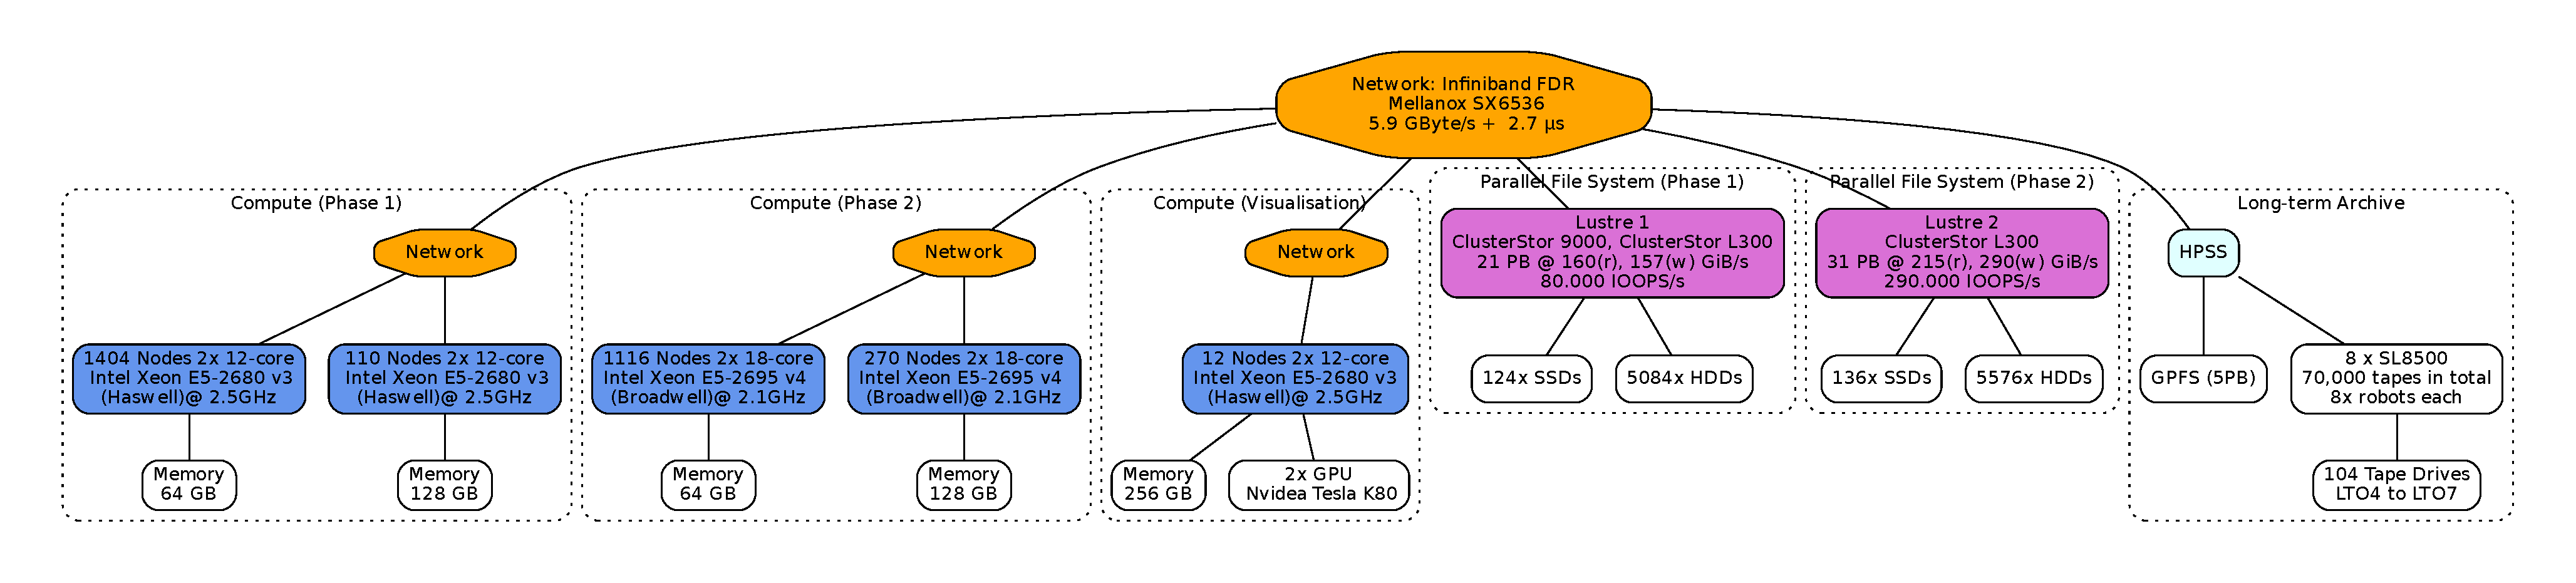
\includegraphics[width=\textwidth]{dot/topo-real-dkrz}
	\caption{Simplified fat-tree topology of DKRZ}
	\label{fig:dkrz topology}
\end{figure}



\begin{table} [htbp]
\centering
\small
\begin{tabular}{|l||lll|}
	\hline
	                   & 2004      & 2009      & 2015        \\ \hline
	Performance        & 1.5 TF/s  & 150 TF/s  & 3.1 PF/s    \\
	Nodes              & 24        & 264       & 2882        \\
	Node performance   & 62.5 GF/s & 0.6 TF/s  & 1.0 TF/s    \\
	System memory      & 1.5 TB    & 20 TB     & 200 TB      \\
	Network links      & -         & -         & 3100        \\ \hline
	Storage	capacity   & 100 TB    & 5.6 PB    & 52 PB       \\
	Storage	throughput & 5 GB/s    & 30 GB/s   & 700 GB/s    \\
	Storage servers    & 1         & 12        & 130         \\
	Disk drives        & 4000      & 7200      & 10600       \\ \hline
	Archive	capacity   & 6 PB      & 53 PB     & 500 PB      \\
	Archive	throughput & 1 GB/s    & 9.6 GB/s  & 18 GB/s     \\ \hline
	Power consumption  & 250 kW    & 1.6 MW    & 1.2 MW      \\
	Investment         & 26 M\euro & 35 M\euro & 38.5 M\euro \\ \hline
\end{tabular}
 \caption{DKRZ System characteristics}
 \label{tbl:dkrz characteristics}
 \vspace*{-0.35cm}
\end{table}


\begin{table}
\centering
\begin{tabular}{|l|r|r|}
	\hline
	         &   Investment & Power consumption \\ \hline
	Compute  & 15.75 M\euro &           1100 kW \\
	Network  &  5.25 M\euro &             50 kW \\
	Storage  &   7.5 M\euro &            250 kW \\
	Archive  &     5 M\euro &             25 kW \\
	Building &     5 M\euro &                -- \\ \hline
\end{tabular}
\caption{Potential investment costs and power consumptions for DKRZ}
\label{tbl:dkrz model costs}
\vspace*{-0.35cm}
\end{table}


%%%%%%%%%%%%%%%%%%%%%%%%%%%%%%%%%%%%%%%%%%%%%%%%%%%%%%%%%%%%%%%%%%%%%%%%%%%%%%%

\subsection{Example Data Centre: STFC JASMIN}
\label{sec:STFC current}

The STFC scientific computing department runs services for a number of customers, here we concentrate on the physical systems which underpin environmental science, and in particular, the JASMIN system.  JASMIN shares a physical data centre with other large computing activities, and in particular, the UK LHC Tier 1 centre, and the STFC tape archive - which itself serves a range of clients.

\begin{figure} [p]
	\centering
	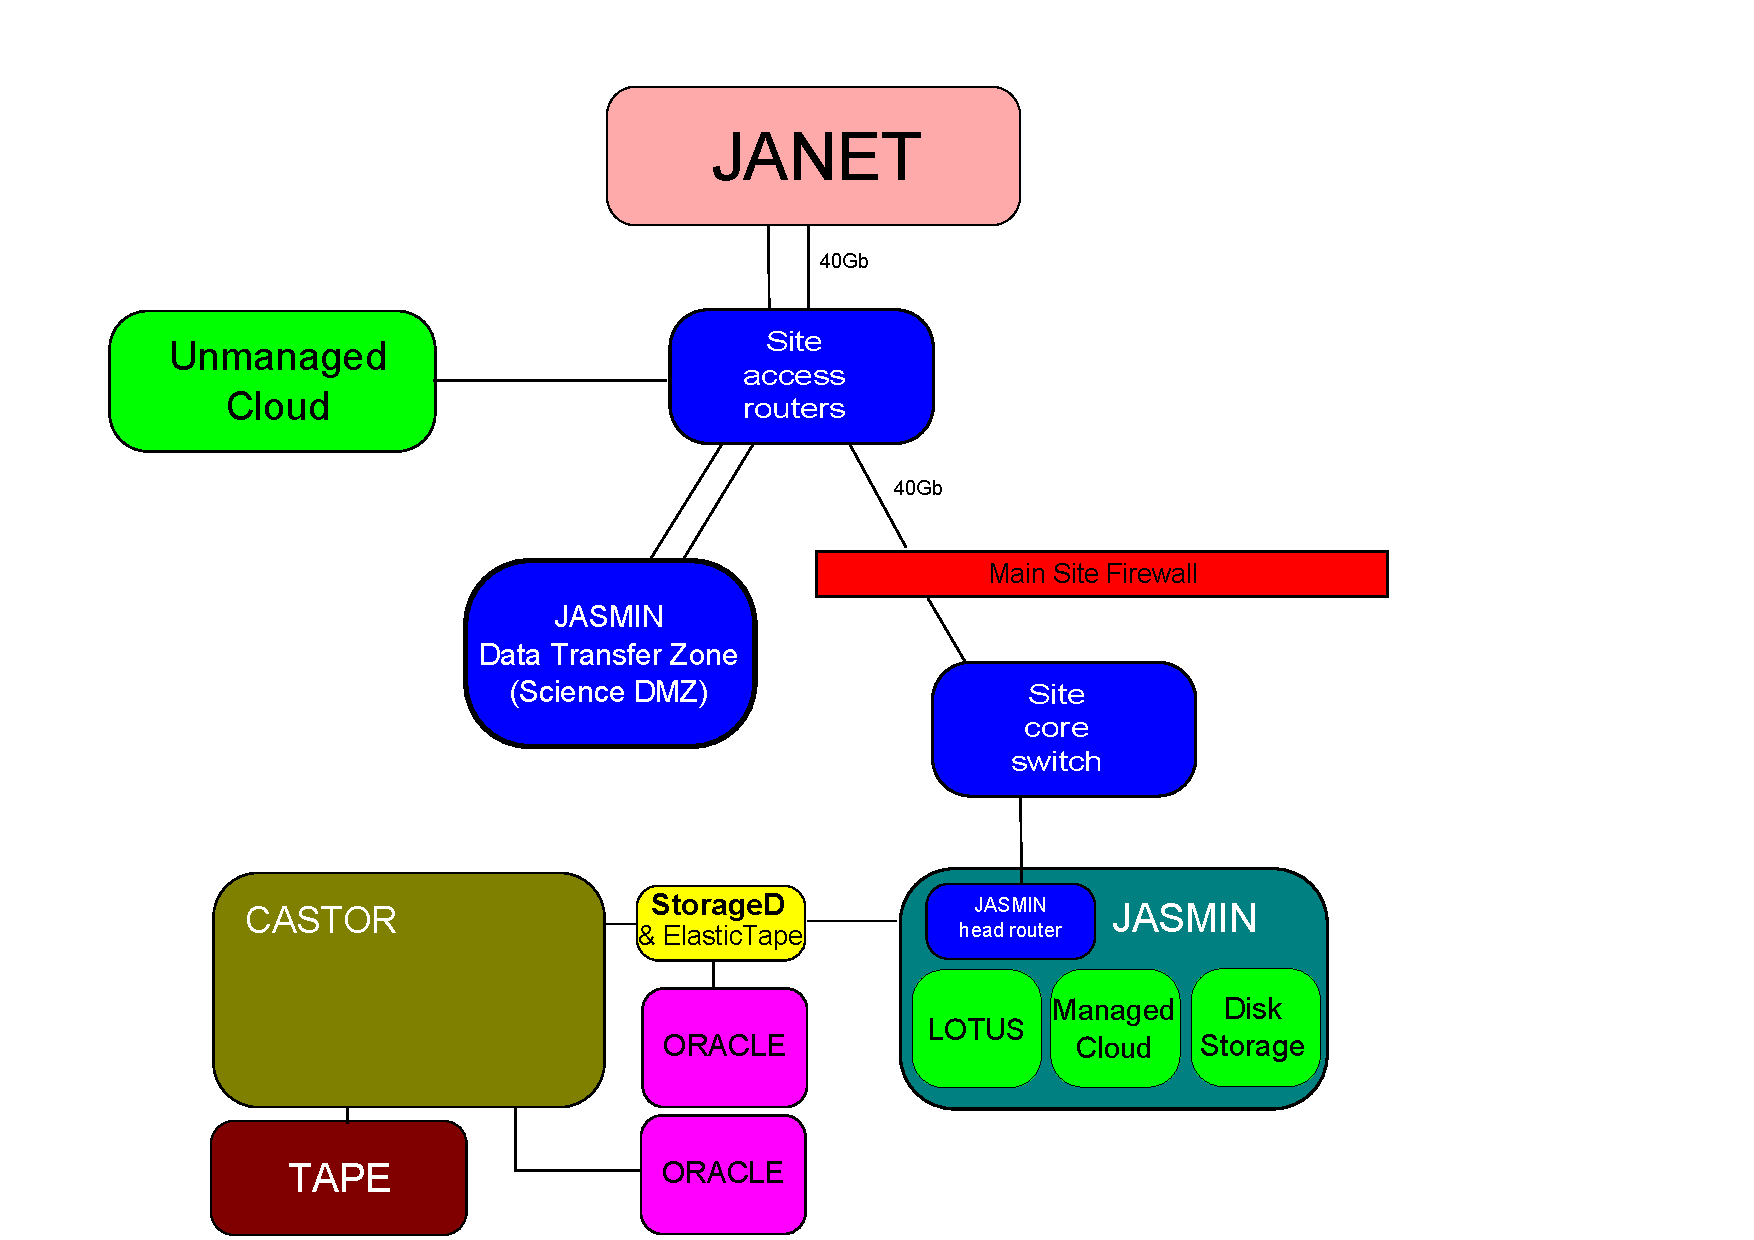
\includegraphics[width=0.7 \textwidth]{figures/topo-real-stfc}
	\caption{Schematic view of the JASMIN infrastructure, including the interfaces to the STFC tape library systems.}
	\label{fig:topostfc}
\end{figure}


\begin{table} [p]
  \centering
  \begin{tabular}{|l|r|r|r|}
    \hline
    JASMIN		&	Phase 1		& Phase 2	& Phase 3	\\
    Date		&	2013		& 2014		& 2015-16	\\
    \hline
    Cores (Cloud)	&	504		& $\ddagger$		& 816		\\
    Cores (LOTUS)	&	144		& $\ddagger$		& 4880		\\
    Cores (Dedicated) &     $\ddagger$ & $\ddagger $ & 120 \\
    Mem/Node (LOTUS)	&	48/256 GB	& 128/512 GB	& 128/512 GB	\\
    Network		&	Gnodal		& Mellanox	& Mellanox	\\
    NetApp storage	&	0.07 PB		& 0.9 PB	& 1 PB		\\
    Panasas storage	&	5 PB		& 6.9 PB	& 16 PB		\\
    Storage-D Tape Capacity$\dagger$ (CEDA)&	 $\ddagger$	& $\ddagger$	& 9 PB	\\
    Elastic Tape Capacity$\dagger$ (JASMIN)& $\ddagger$&  $\ddagger$	& 26 PB	\\
    Offsite Tape Capacity                                 &         $\ddagger$          &   $\ddagger$    & 8 PB \\
    \hline
     \end{tabular}
     \begin{center}
  $\dagger$: Based on the number of tapes owned and installed in the shared STFC tape library.\\
    $\ddagger$: Capacity has not always been constant in previous phases as resources were being moved between categories.  \end{center}
  \caption{STFC JASMIN/CEDA resources at some of the major stages of evolution. Note that the
  memory configurations vary significantly, from 48 GB to 2048 GB/node (with only a few of the  2 TB nodes for special use cases). \\
}
  \label{table:stfc}
\end{table}


JASMIN  consists of several logical and physical subsystems serving a range of ``tennancies'', that is, client communities. The most important of those tenancies delivers the petascale curated archive and associated services for the Centre for Environmental Data Analysis (CEDA), however, there are many other tenancies whose use cases range from sharing storage with access to batch computing, to exploiting IaaS cloud services.  The CEDA archive interfaces with the STFC tape archive through the ``Storage-D'' interface, while other tenancies can access the tape archive through the ``Elastic Tape'' interface (so called because the provision of tape is elastic in the cloud sense). Both JASMIN tape interfaces provide cache interfaces to the underlying CASTOR system (and it's own cache), but differ in the software implementation and supported workflows.

Key components of the physical system include a heterogeneous batch cluster (LOTUS, with a range of hardware purchased in several phases), two pools of hypervisors which support several distinct private clouds(the most important of which are the ``managed cloud'' providing PaaS administered by CEDA and the ``unmanaged cloud'' providing IaaS), the main storage pool (one PANASAS\texttrademark\ file system, albeit in pools of different generation hardware purchased in several phases), and block storage to support the private clouds. The entire system is connected with a high performance internal network.

\Cref{fig:topostfc} shows a (slightly simplified) view of the STFC infrastructure for JASMIN (the specifics being
listed in \Cref{table:stfc}).  JANET is the UK NREN, and STFC's data centre for JASMIN has dual connections to
JANET (for redundancy more than bandwidth, as the backup connection goes via a different MAN).  Site access routers
(SARs) also manage OPNs (JASMIN has three OPNs, one to the Met Office for HPC access, one to the University of Leeds, and one to the Edinburgh Parallel Computer Centre also for HPC access, but these are not shown for simplicity).  There are at least two Data Transfer Zones (see
\Cref{sec:dmz}), one of which supports JASMIN; these are connected to the SARs, the one for JASMIN provides a GridFTP endpoint which is registered with Globus.

The data service -- on the bottom LHS of \Cref{fig:topostfc} -- is based on two SL8500 StorageTek libraries in maximal
extent, 10,000 slots each.  Essentially one robot supports the LHC, and the other supports everyone else, including the
CEDA data archive and the JASMIN storage services.  Tape media are T10KC and D, with capacities of, respectively, 5TB
and 8.5TB (prior to compression), so the nominal (uncompressed) capacity of each library is 85~PB. Tape library clients such as JASMIN and CEDA purchase their own tapes in the libraries so as to have their own maximal capacity.


%\todo{as well as associated costs + progniss on scale of future systems? }


%%%%%%%%%%%%%%%%%%%%%%%%%%%%%%%%%%%%%%%%%%%%%%%%%%%%%%%%%%%%%%%%%%%%%%%%%%%%%%%
%\comment{
%\subsection{Example Data Center: ??? italy}
%
%\todo{italy data center ?}
%}

%%%%%%%%%%%%%%%%%%%%%%%%%%%%%%%%%%%%%%%%%%%%%%%%%%%%%%%%%%%%%%%%%%%%%%%%%%%%%%%

\section{Compute + Parallel File System + Tape}
\label{sec:compute + pfs + tape}


%\begin{figure}[]
%	\centering
%	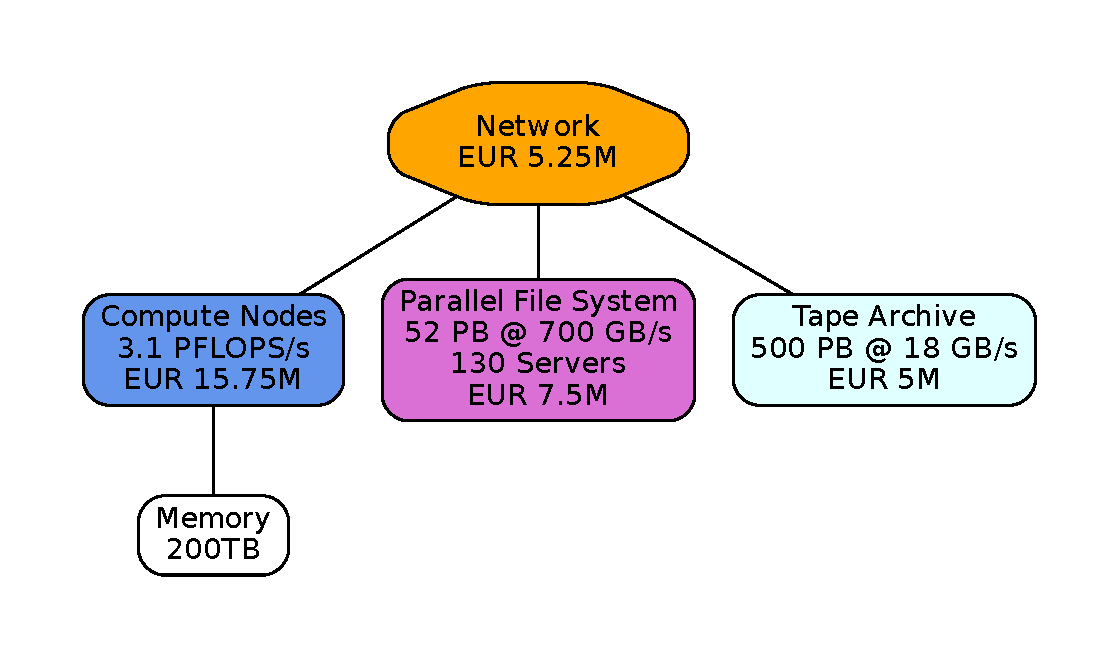
\includegraphics[scale=0.49]{dot/topo-compute+pfs+tape+COST}
%	\caption{}
%	\label{fig:topology compute + pfs + tape}
%\end{figure}

The status quo at DKRZ is the system described in \Cref{sec:DKRZ current}. Here we investigate changing
the proportions of the individual storage subsystems. Given that the disk systems are purchased independently
of the tape systems, at different times, there is a natural technological mismatch.

The costs for this scenario in comparison to the baseline system (see \Cref{sec:DKRZ current}) is listed in \Cref{tbl:costsforcomputepfstape}.
%\Cref{tbl:benefits for compute + pfs + tape} summarizes and rates the changes by their impact to the various use cases (see \Cref{sec:use cases}).
\Cref{fig:topology compute + pfs + tape} provides a quick visual overview of this architecture.
Lets begin by establishing the price per terrabyte and year for tape and disk in a current deployment.

\begin{figure}[h]
	\centering
	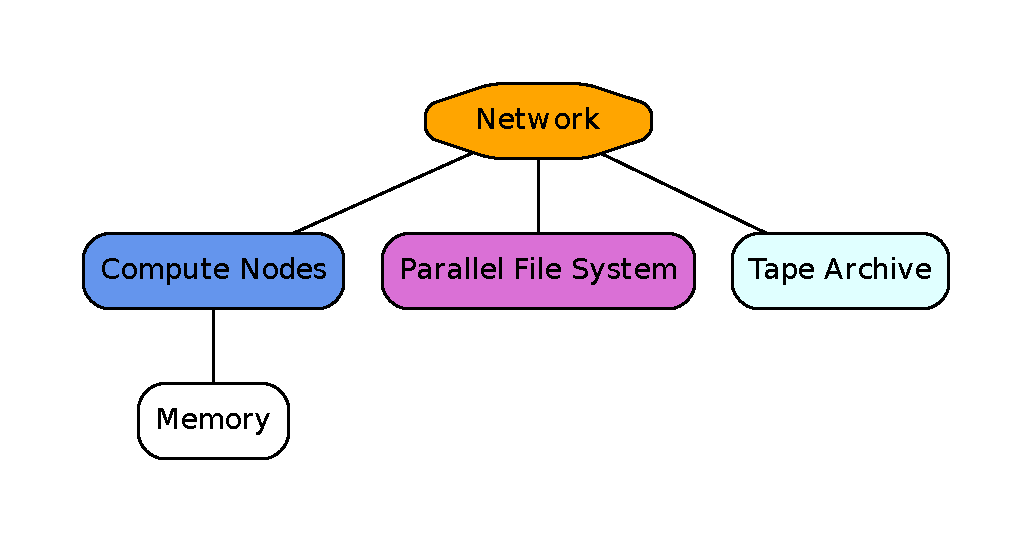
\includegraphics[scale=0.49]{dot/topo-compute+pfs+tape}
	\caption{Topology for the traditional case: Compute + File System + Tape}
	\label{fig:topology compute + pfs + tape}
\end{figure}

%\comment{
%media is constantly replace..
%
%	every year.. about 6000 tapes replaced
%
%	thus.. 70000 * 6000 *
%
%invisible to our operations.. but tape drives fail pretty regulary.. every month.. and need maintenaince.. which is the maintence contracts are there...
%
%
%hpss, was procured with the other systems..  and also is in its second generation already..
%	originally power arch
%	but now x86
%
%also mentioned is a pricing policy shift..
%	where Sun and other would grant generous discounts to academic users...
%		that in regard to the low media prices
%
%
%}



\paragraph{Tape Cost (TB/Y, EUR):}
\label{calc:TAPE EUR/TB/Y}

%\todo{JJ: "huge" $rightarrow$ "signficant"?}
To operate a tape system it is necessary to commit to a huge upfront investment for the tape system.
The DKRZ operates 7 StorageTek SL8500 library complexes with 3 library units on site and an additional library unit procured together with the others as an offsite backup in Garching.
The tape infrastructure does not age as quickly as compute or storage systems do as cartridges, robot systems and drives remain compatible even as tape media evolves.
For the current system it seems fair to assume that the tape archive infrastructure remains usable for 2-3+ generations of supercomputers.
This is due to two main factors: 1) the current configurations does not exhaust all the available drive slots 2) as tape media increases in capacity with each new generation of tape media there is the potential to reclaim a significant number tape slots.
Tape technologies and futures will be covered in further detail in D4.4.

Lets assume each SL8500 module equipped with about 20 drives will cost slightly under 1M EUR, thus 7M EUR for DKRZ but assume it can be used for 3 generations reducing it to 2.3M EUR investment costs for the life time of one supercomputer.
As the tape storage requires a license for HPSS and storage cache with some support for the library and the software; let us assume a total investment of 7.5M EUR for the life time of the system. 
Staffing requires three specialists, assume an operational budget for DKRZ of about 3M EUR, and assuming 3 staff are 5\% of that total, the annual cost is 150 kEUR.   
In addition, the floor space to keep the system is equivalent to 70k EUR per year.
We neglect the cost to maintain the oxygen reduction environment here.
This adds up to 8.6M EUR over the life time of the system.
Thus, for each of our 67,000 tape slots, we roughly pay 128.36 EUR per supercomputer generation (and 5 years) or 25.70 EUR per year.

Assume a tape medium costs about 20 EUR and can be used for 5 years. 
The investment of tape medium and costs per slot space would sum up to the costs of 30 EUR per year and tape.
With 2.5 TByte of raw capacity for an LTO-6 tape, this would sum up to 12 EUR/TB/Y. 
As practice shows, on one hand, the embedded compression may yield a compression ratio of 1.5 but, on the other hand, 
empty space due to deleted files may compensate for this leading to a realistic cost of 12 EUR/TB/Y.

%\comment{
%oben bei Tape beschreiben:
%\todo{real cost for tape system since procurement}
%fixed costs ca 1 Mio pro Library block, 5 Mio, für 2-3 Supercomputer generationen
%5 MIo für die Laufzeit des Supercomputers
%ca. 7.5 MIO Investment für Laufzeit
%Anzahl Personen nötig für Tape ? ca. 3 Personen == 5% DKRZ Staff costs, plus Raum, für 5 Jahre, ca. 0.75 Mio für die Laufzeit
%ca. 10 MIO für alles, 2 MIO pro Jahr für den Betrieb. 70000, stellfläche kostet:
%- 142 Euro pro Stellplatz und Jahr, 6 TByte == 23 EUR (unkomprimiert) für ein Jahr,
%Tape medium 20 EUR, sagne wir mal für 5 Jahre gut, 4 EUR pro Jahr drauf: 27 EUR pro TB / Jahr
%21.25 EUR pro TB OHNE Kosten für Staff und Gebäude usw.
%}


\paragraph{PFS Cost (TB/Y, EUR):}
\label{calc:PFS EUR/TB/Y}

To put this price into perspective, we need also need to consider the price per TB for online storage in parallel file systems.
EUR 7.5M and a expected system life of 5 years bought 52 PB for the storage servers and storage media.

$$7.5\mathrm{M EUR} / 52 \mathrm{PB} / 5 \mathrm{Years} = 28.17 \mathrm{EUR/TB/Year}$$

As this does not account for staff, facility and most importantly power consumption. So lets assume 250KW which would cost 400k EUR/Year thus increasing the price for a TB/Year to to roughly 36 EUR.
This does neglect that the files system will be underutilized in the beginning.


%\todo{gamme a 95\%... filling level..}

%\comment{
%The parallel file system is
%
%52 PByte  / (7.5 M Euro (for 5 years) / 5 year (lifetime)) => 34.7 PBs per million and year
%=> 28.8 EUR pro Terrabyte and year idle costs, d.h. for a HDD with 3 TByte one would pay 75 EUR per year.
%Es kommt noch Personen und Building Kosten dazu, auch Energiekosten ....
%Sagen wir mal 250 KW == 400 k = 1.9 MIO pro Jahr == 36.5 EUR
%
%Gamma dazu rechnen, sagen wir mal 95% voll (gerade am Anfang eines neuen Dateisystems ist das doch recht leer), später durchaus immer zu 99% voll
%}


\subsection{Potential for optimization}

\paragraph{Reduced Online Storage Budget}
For this scenario lets assume we would like to reduce the storage footprint on the budget.
For example if we cut our storage spending in half, in the case of DKRZ, that would amount to EUR 3.75M that can be spent elsewhere.
That corresponds to about 24\% of the cost of the compute system and we can expect an similar increase in performance at the disposal for scientists.
This would translate into 686 additional nodes and thus would add about 0.74 PFLOPS of performance to the system, while 65 storage nodes (+600 connections) are removed in comparison to the reference.

We can not change the compute system without also making changes to the network lets approximate the optimization process necessary to find a realistic investment.
The network costs would increase by $(3100 + 686 - 65) / 3100 = 1.20 = 1.05 \mbox{M EUR}$, which combined is beyond the budged.
If we choose to instead invest EUR 3M in to compute, accounting for only  540 nodes and a 10\% performance increase.
Now can afford a network to support the additional hardware with a additional network cost of $ network_{cost} \cdot 1.156 = 6 \mbox{M EUR}$.
The increase in power is not necessarily proportional so lets assume a increase in power consumption of roughly 10%.
The changes may affect how user will work.
By shrinking the online storage architecture, also the maximum working set is smaller.
For example jobs potentially should specify when to stage/unstage data.
Staging mechanisms in many cases maybe be automated by Slurm thus making staging transparent to the users.


%
%\comment{
% Less online storage, migrating more idle data to tape:
%
%Assumption: We spend half the money for storage in compute (and potentially in the archive).
%storage - 50\%.
%3.75 M euro, corresponds to 24\% of the compute costs, theoretically \% more science.
%Means + 686 nodes + 0.74 PF/s. - 65 storage nodes (+600 connections), d.h. network, 3100 network + 621 connections.
%However, the network costs would increase as well by $(3100 + 686 - 65) / 3100 = 1.20 = 1.05M EUR$.
%
%With 3 M euro in the compute, 19\% more compute, +540 nodes.
%Network 1.156 = 6 M euro.
%
%
%would increase the power consumption also by roughly 10\%.
%2.5\% performance of the archive vs. the best case of the storage (additional latency).
%Staging embedded into Slurm would allow batch jobs to run with regular speed hidden from the user.
%Alternatively 2.5 million improving the archive, two new complexes.
%
%Smaller working set on storage.
%Users have to adjust jobs to potentially stage / unstage data.
%}




\begin{table}
\centering
\begin{tabular}{|l|r|r|r|}
	\hline
	Characteristics    &        Value & Factor & New value \\ \hline
	Performance        &     3.1 PF/s &   1.19 &  3.7 PF/s\\
	Nodes              &         2882 &   1.19 &  3430\\
	Node performance   &     1.0 TF/s &        &  \\
	System memory      &       200 TB &   1.19 &  238\\
	Network links      &         3100 &   1.15 &  3565\\ \hline
	Storage	capacity   &        52 PB &    0.5 &  26 PB\\
	Storage	throughput &     700 GB/s &    0.5 &  350 GB/s\\
	Storage servers    &          130 &    0.5 &  65\\
	Disk drives        &        10600 &    0.5 &  5300\\ \hline
	Archive	capacity   &       500 PB &        &  \\
	Archive	throughput &      18 GB/s &        &  \\ \hline\hline
	Compute costs      & 15.75 M EUR &   1.24 &  19.53 M EUR\\
	Network costs      &  5.25 M EUR &   1.15 &  6.04 M EUR\\
	Storage costs      &   7.5 M EUR &    0.5 &  3.75 M EUR\\
	Archive costs      &     5 M EUR &        &  \\
	Building costs     &     5 M EUR &        &  \\ \hline
	Investment         &  38.5 M EUR &        &  \\ \hline
	Compute power      &      1100 kW &   1.19 &  1309 kW\\
	Network power      &        50 kW &        &  \\
	Storage power      &       250 kW &    0.5 &  125 kW\\
	Archive power      &        25 kW &        &  \\ \hline
	Power consumption  &       1.2 MW &        &  \\ \hline
\end{tabular}
\caption{Projected costs for the Scenario Compute + Parallel File System + Tape; subscenario: half the storage. Note that this demonstrates the feedback between node count and network costs.}
\label{tbl:costsforcomputepfstape}
\end{table}


\comment{
\begin{table}
\centering
\small{
\begin{tabular}{ |l|| c|c|c|c || c|c|c|c|c| }
	\hline
	                         & \multicolumn{4}{c||}{\textbf{Climate}} & \multicolumn{5}{c|}{\textbf{Weather}} \\ \hline
	                         & CUC1 & CUC2 & CUC3 &       CUC4        & WUC1 & WUC2 & WUC3 & WUC4 &   WUC5   \\ \hline\hline
	\textbf{Characteristics} &      &      &      &                   &      &      &      &      &  \\ \hline
	Throughput               &      &      &      &                   &      &      &      &      &  \\ \hline
	Latency                  &      &      &      &                   &      &      &      &      &  \\ \hline
	Capacity                 &      &      &      &                   &      &      &      &      &  \\ \hline
	Resilience               &      &      &      &                   &      &      &      &      &  \\ \hline\hline
	\textbf{Cost}            &      &      &      &                   &      &      &      &      &  \\ \hline
	Initial                  &      &      &      &                   &      &      &      &      &  \\ \hline
	Energy                   &      &      &      &                   &      &      &      &      &  \\ \hline
	Other                    &      &      &      &                   &      &      &      &      &  \\ \hline
\end{tabular}
}
\caption{Benefits }
\label{tbl:benefits for compute + pfs + tape}
\end{table}
}

%%%%%%%%%%%%%%%%%%%%%%%%%%%%%%%%%%%%%%%%%%%%%%%%%%%%%%%%%%%%%%%%%%%%%%%%%%%%%%%

\section{Compute + Object Storage (+ Tape)}
\label{sec:compute + objects + tape}

\begin{figure}[]
	\centering
	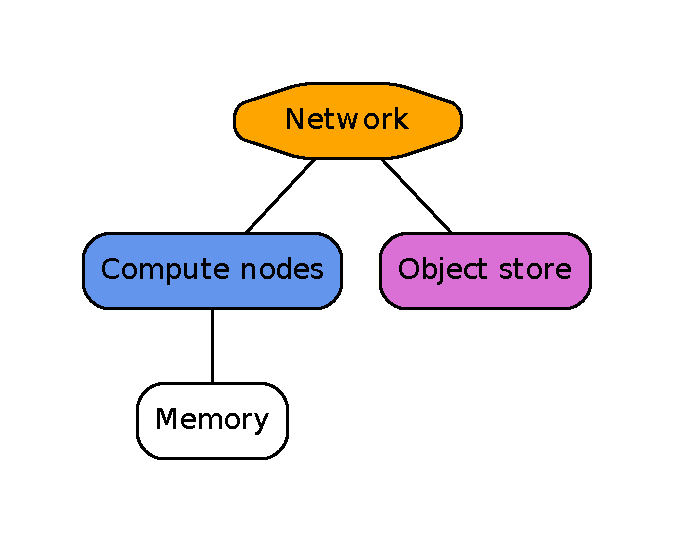
\includegraphics[scale=0.49]{dot/topo-compute+objects}
	\caption{Topology for the case where object storage replaces the parallel file system}
	\label{fig:topology compute + objects + tape}
\end{figure}

In this section we explore two questions:
Object stores promise higher performance at lower cost than parallel file systems as commodity hardware can be used. What are the cost savings we can expect when switching to object stores.
To exploit object stores applications will need to change to some extend how data is stored. In \Cref{sec:towards esd}
we illustrate how this transition maybe made less disruptive to the community.
The costs for this scenario in comparison to the baseline system (see \Cref{sec:DKRZ current}) is listed in \Cref{tbl:costs compute + objects + tape}.
%\Cref{tbl:benefits compute + objects + tape} summarizes and rates the changes by their impact to the various use cases (see \Cref{sec:use cases}).
\Cref{fig:topology compute + objects + tape} provides a quick visual overview of this architecture.



\paragraph{Object Storage vs. Parallel File Systems}

Lets assume usual idle storage costs are indeed in the order of 36.5 EUR / TB / year (\Cref{calc:PFS EUR/TB/Y}).
HPC hard drives are usually more expensive as they come with additional guarantees.
At the moment, an 8 TB disk will cost about 260 EUR, or 32.5 EUR per TB.
Assuming a life time without failure of 5 years, that is 6.5 EUR per TB and year.
In a typical server, there maybe slots for up to 80 hard drives at a cost of about 3000 EUR per server.
For a configuration with 8 TB disks, this adds another 1 EUR per TB per year.
Energy consumption of such a server (including disks) would be in the order of 400 Watts or 5 EUR per HDD and year (under active I/O, the system may actually consume a bit more energy, but let us neglect this here).

Thus, overall an object storage server could host storage with a cost of 12.5 EUR per TB and year, slightly more expensive than tape with 12 EUR per TB and year.
However, usually some kind of redundancy is needed, with declustered RAID-6 and a 8+2 configuration, 25\% of additional space is needed for redundancy. 
But this is true for tape as well.

Note that the object storage, however, does not take into account any software licensing costs\footnote{Assuming we use open source and free software such as Ceph.} or staff considerations as we have done for tape.
So in practice, the costs for object storage is actually a bit higher.
%Some vendors actually said object storage might cost about 1/2 of the original HPC storage, so the overall calculation seems to point in the right direction.

%
%\comment{
%Normal idle storage costs so was wie: 36.5 EUR pro TByte / year
%
%HPC Platten, Object storage platten sind billiger.
%Aktuell: 8 TByte Server Platte ca. 260 EUR, 32.5 EUR pro TByte in 5 Jahren => 6.5 EUR pro Jahr (falls nix kaputt geht).
%Server für 80 Platten kostet 3000 EUR == 37.5 EUR pro Stellplatz == 7.5 EUR pro Jahr.
%14.0 EUR pro Jahr
%Man könnte zu Object store für den halben Preis kommen.
%== 6500 Platten.
%Kosten für Server selber bleiben gleich.
%
%=> 81 Server anstelle 130.
%Falls jeder gleiche Leistung liefern würde, dann wäre es 81/130 = 60% der Originalleistung
%Aber wir sagen mal
%
%Keine Redundanz hier!!!
%10+2 => +20 Platten und Server
%=> 7800 Platten, 98 Server => Leistung ist 75% der Originalleistung, aber billigkram => nur 1/2 Leistung angenommen => 37.5% der Leistung
%
%=> 75% der Storage Ressourcen benötig, Platten zu halbem Preis
%
%=> gerne auch mal konkret aussrechnen:
%-- (98*3000+7800*260) = 2,3 MIO
%=> Preis für aktuellen Object storage ist wenigstens 30% von dem Preis den wir früher bezahlt haben.
%Manufacturing costs and software stuff, 3.75 Mio for the object storage feels OK.
%=> Overall: lets assume half the price for the storage...
%
%
%



\paragraph{Replacement of tape with object storage}

While would be certainly interesting to switch to a model where tape is replaced with object storage, there are some obstacles.
Remember, the 67,000 tape slots (LTO-6) of DKRZ virtually provide as much space as 21,000 (8 TB) HDDs or 261 object storage servers (sth. like 27 racks of servers).
From the overall energy consumption, this would take about 100 kW; the tape library requires less energy with about 2,000 Watts per SL8500 library\footnote{
It is actually between 1.2 kW (idle) and 4.8 kW (active) according to Oracles Power Calculator \url{http://www.oracle.com/us/products/servers-storage/sun-power-calculators/}.}, but the additional HPSS servers and storage reduces the gap.
Cost-wise the gap is not too high.

One benefit of the tape archive is that it can be gradually upgraded by hosting different generations of tape in one library.
This could be realized with object storage theoretically as well.
Another benefit of tape is that  media fail rarely compared to even enterprise disks, allowing to reduce the required level of redundancy.
Still, based of these calculations it seems to be appealing to consider means to either reduce the costs for the tape archives by applying more feasible models or to deploy price competetive object storage.



\begin{table}
\centering
\begin{tabular}{|l|r|r|r|}
	\hline
	Characteristics    &       Value & Factor &  New value \\ \hline
	Performance        &    3.1 PF/s &   1.19 &   3.7 PF/s \\
	Nodes              &        2882 &   1.19 &       3430 \\
	Node performance   &    1.0 TF/s &        &  \\
	System memory      &      200 TB &        &  \\
	Network links      &        3100 &        &  \\ \hline
	Storage	capacity   &       52 PB &        &  \\
	Storage	throughput &    700 GB/s &  0.375 &   262 GB/s \\
	Storage servers    &         130 &   0.75    &         98 \\
	Disk drives        &       10600 &   0.74  &       7800 \\ \hline
	Archive	capacity   &      500 PB &        &  \\
	Archive	throughput &     18 GB/s &        &  \\ \hline
	Compute costs      & 15.75 M EUR &        &  \\
	Network costs      &  5.25 M EUR &   0.98 & 5.15 M EUR \\
	Storage costs      &   7.5 M EUR &    0.5 & 3.75 M EUR \\
	Archive costs      &     5 M EUR &        &  \\
	Building costs     &     5 M EUR &        &  \\ \hline
	Investment         &  38.5 M EUR &        &  \\ \hline
	Compute power      &     1100 kW &        &  \\
	Network power      &       50 kW &        &  \\
	Storage power      &      250 kW &   0.75 &     188 kW \\
	Archive power      &       25 kW &        &  \\ \hline
	Power consumption  &      1.2 MW &        &  \\ \hline
\end{tabular}
\caption{Projected costs for the Scenario Compute and Object Lets assume DKRZ still handles compute jobs on site, then this would require to
	Storage; replace online storage with cheaper object storage}
\label{tbl:costs compute + objects + tape}
\end{table}


\comment{
\begin{table}
\centering
\begin{tabular}{|l|| c|c|c|c || c|c|c|c|c|}
	\hline
	                         & \multicolumn{4}{c| |}{Climate} & \multicolumn{5}{c|}{Weather} \\ \hline
	                         & UC1 & UC2 & UC3 &     UC4      & UC1 & UC2 & UC3 & UC4 & UC5  \\ \hline\hline
	\textbf{Characteristics} &     &     &     &              &     &     &     &     &  \\ \hline
	Throughput               & -   &  -  &     &              &     &     &     &     &  \\ \hline
	Latency                  & -   &  -  &     &              &     &     &     &     &  \\ \hline
	User experience          & =   &  =  &     &      -       &     &     &     &     &  \\ \hline
	Capacity                 & NA  & NA  &     &              &     &     &     &     &  \\ \hline
	Resilience               & xx  &     &     &              &     &     &     &     & \\ \hline
\end{tabular}

\caption{}
\label{tbl:benefits compute + objects + tape}
\end{table}
}


%%%%%%%%%%%%%%%%%%%%%%%%%%%%%%%%%%%%%%%%%%%%%%%%%%%%%%%%%%%%%%%%%%%%%%%%%%%%%%%

\section{Compute + Object Storage + Cloud}
\label{sec:compute + objects + cloud}

\begin{figure}
	\centering
	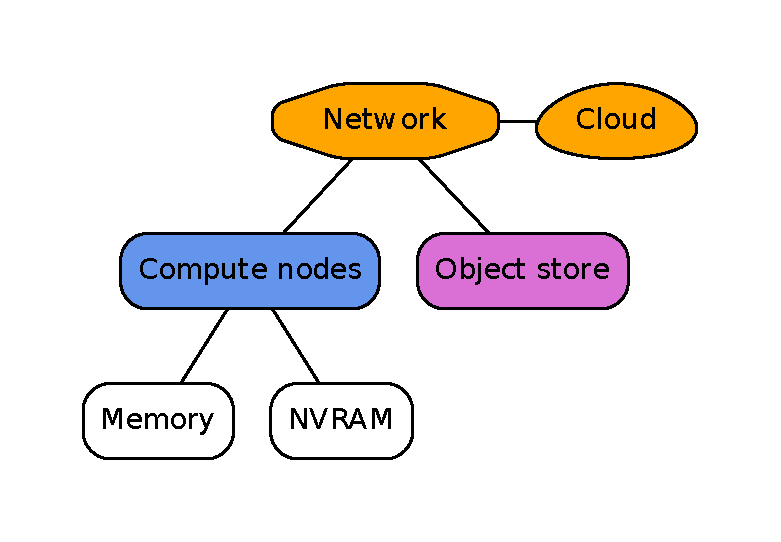
\includegraphics[scale=0.49]{dot/topo-compute+object+cloud}
	\caption{Topology for the case with object storage and external cloud storage}
	\label{fig:topology compute + objects + cloud}
\end{figure}


Another interesting scenario is to size the on site system to match the normal operations and use cloud resources when the available system do not suffice. There are two main perspectives to this approach: 1) side step for compute and avoid seldom used special purpose hardware 2) archive in the cloud with potentially superior data safety and availability.
%The costs for this scenario in comparison to the baseline system (see \Cref{sec:DKRZ current}) is listed in \Cref{tbl:costs compute + objects + cloud}.
%\Cref{tbl:benefits compute + objects + cloud} summarizes and rates the changes by their impact to the various climate and weather use cases (see \Cref{sec:use cases}).
\Cref{fig:topology compute + objects + cloud} provides a quick visual overview of this architecture.

%\Cref{fig:topology compute + objects + cloud + COST}



\paragraph{Cloud currently not feasible for large scale archival}

Many clouds services promise to provide better data protection and availability than conventional or self hosted solutions.
For small to medium scale, infrequently accessed data this business case may indeed be true.
Especially as cloud allows to scale throughput and capacity freely, albeit at the cost of a less predictable performance due ignorance about the underlying architecture.
This scenario will consider cloud as an alternative to replace an in house tape archive for long-storage.

Amazon Glacier is currently  one of the cheapest cloud storage options, and is priced at 0.4 cents per month, resulting in 48 \$ per TB/Year which compares poorly with the cost of on-site PFS calculated above, let alone tape.  However, even if some sort of special deal was possible which reduced the cost of storage to zero, Glacier retrieval also incurs costs.  Given retrieval costs currently at $0.003$\$/GB, this suggest retrieval costs alone of some multiple of (3\$/TB)  in the first year (although retrievals might fall in subsequent years), a number which itself could become comparable with on-site object storage!

500 PB would cost nearly 25 M\$ per year,  before considering actually using the data!

%	Table with different cloud providers:
%	Glacier: 0.4 cents per month and gbyte => 48 \$ pro Terrabyte und Jahr
%	Access costs of 9 cents per Gbyte ignored ...
%
%	Amazon standard: 2.3 cents
%	276 \$
%
%	"Ingest" costs since HPC is at home, and storage in the cloud.
%	Einmal zugriff auf 1 TB: 90 \$
%
%
%	What happens if we move compute into the cloud:
%
%	https://pod.penguincomputing.com/pricing
%
%
%
%	core hr: \$0.08
%	DKRZ produces core hours: 2882 nodes with 24 cores / 36 cores pro node
%	Utilization von 0.9 für DKRZ. 22,721,688 core hours are produced.
%	1.82 M Euro * 30 ca. 54.4 MIO EURO pro Jahr Compute da...
%	ca. 10x kosten, delta faktor




\comment{
\begin{table}
\centering
\begin{tabular}{|l|| c|c|c|c || c|c|c|c|c|}
	\hline
	                         & \multicolumn{4}{c| |}{Climate} & \multicolumn{5}{c|}{Weather} \\ \hline
	                         & UC1    & UC2 & UC3 &    UC4    & UC1 & UC2 & UC3 & UC4 & UC5  \\ \hline\hline
	\textbf{Characteristics} &        &     &     &           &     &     &     &     &  \\ \hline
	Throughput               & -      &  -  &     &           &     &     &     &     &  \\ \hline
	Latency                  & --     &  -  &     &           &     &     &     &     &  \\
	User experience          & =      &  =  &     &     -     &     &     &     &     &  \\ \hline
	Capacity                 & NA     & NA  &     &           &     &     &     &     &  \\ \hline
	Resilience               & 99.999 &     &     &           &     &     &     &     &  \\ \hline\hline
	\textbf{Cost}            &        &     &     &           &     &     &     &     &  \\ \hline
	Initial                  & =0     & =0  &     &           &     &     &     &     &  \\ \hline
	Energy                   & =0     & =0  &     &           &     &     &     &     &  \\ \hline
	On demand                & --     &     &     &           &     &     &     &     &  \\ \hline
\end{tabular}
\caption{}
\label{tbl:benefits compute + objects + cloud}
\end{table}
}


%\url{http://gaul.org/object-store-comparison/}
%\url{https://oit.duke.edu/help/articles/pricing-%E2%80%93-storage}
%
%Szenario: Outsourcing von peak benötigter Leistung in die Cloud
%
%Annahme: 90% Compute Zeit reicht für 99% der Zeit
%=> dannach ist das Cluster zu 100% ausgelastet IMMER.
%1% der Zeit braucht 10% Compute extra.l
%
%Outsourcing in Cloud sinnvoll?
%
%- eigtl. transparent für user, d.h. selbes Betriebsystem, oder container und support im Scheduler für die Überlastsverschiebung
%
%90% des Preises für alles?
%Aber 1% der Leistung kostet ja ca. 10% so viel => kostet gleichviel...
%Plus Overhead für migration von Daten... Datenhaltung ist ja wucher siehe oben.
%=> Nur ein Model für Compute Bound issues, idle data kills price...
%
%Kleinere Facility usw?
%
%2D Graph: Normal Usage % and percentage of overload in %.





%\begin{table}
%\centering
%\begin{tabular}{|l|r|r|r|}
%	\hline
%	Characteristics    &        Value & Factor & New value \\ \hline
%	Performance        &     3.1 PF/s &        &  \\
%	Nodes              &         2882 &        &  \\
%	Node performance   &     1.0 TF/s &        &  \\
%	System memory      &       200 TB &        &  \\
%	Network links      &         3100 &        &  \\ \hline
%	Storage	capacity   &        52 PB &        &  \\
%	Storage	throughput &     700 GB/s &        &  \\
%	Storage servers    &          130 &        &  \\
%	Disk drives        &        10600 &        &  \\ \hline
%	Archive	capacity   &       500 PB &        &  \\
%	Archive	throughput &      18 GB/s &        &  \\ \hline
%	Compute costs      & 15.75 M\euro &        &  \\
%	Network costs      &  5.25 M\euro &        &  \\
%	Storage costs      &   7.5 M\euro &        &  \\
%	Archive costs      &     5 M\euro &        &  \\
%	Building costs     &     5 M\euro &        &  \\ \hline
%	Investment         &  38.5 M\euro &        &  \\ \hline
%	Compute power      &      1100 kW &        &  \\
%	Network power      &        50 kW &        &  \\
%	Storage power      &       250 kW &        &  \\
%	Archive power      &        25 kW &        &  \\ \hline
%	Power consumption  &       1.2 MW &        &  \\ \hline
%\end{tabular}
%\caption{Projected costs for the Scenario Compute + Parallel File System + Tape; subscenario: half the storage}
%\label{tbl:costs compute + objects + cloud}
%\end{table}









%%%%%%%%%%%%%%%%%%%%%%%%%%%%%%%%%%%%%%%%%%%%%%%%%%%%%%%%%%%%%%%%%%%%%%%%%%%%%%%

\section{Compute + NVRAM + Tape}
\label{sec:compute + nvram + tape}

\begin{figure}
	\centering
	\begin{subfigure}[t]{0.49\textwidth}
		\centering
		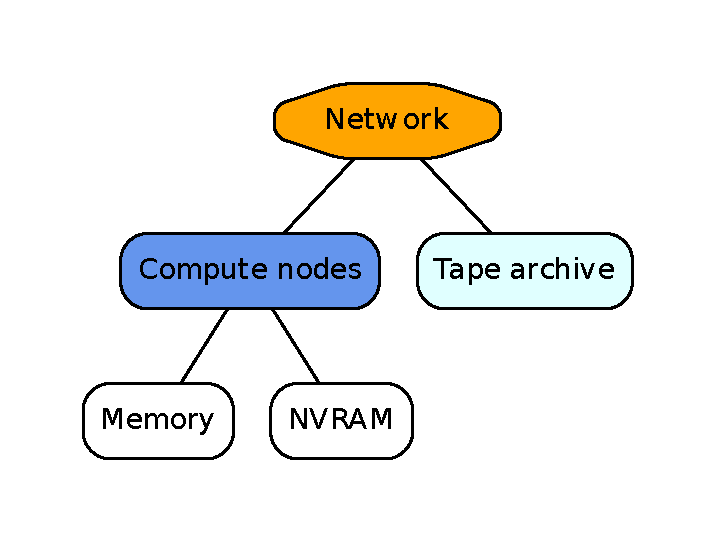
\includegraphics[scale=0.49]{dot/topo-compute+nvram+tape}

		\caption{Node-local NVRAM}
	\end{subfigure}
	\begin{subfigure}[t]{0.49\textwidth}
		\centering
		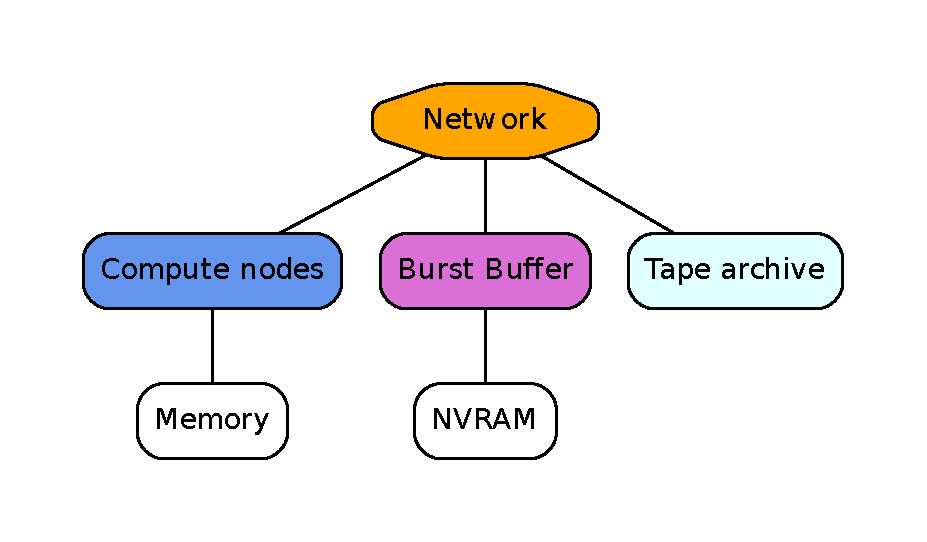
\includegraphics[scale=0.49]{dot/topo-compute+nvram+bb+tape}

		\caption{Shared/Rack-based NVRAM}
	\end{subfigure}


	\caption{Possible integrations of NVRAM + Tape in a data centre.}
	\label{fig:topology compute + nvram + tape}
\end{figure}

\Cref{fig:topology compute + nvram + tape} depicts how a simplified but typical data centre might look like.
In this particular case also NVRAM is in cooperated and is installed near to compute nodes while other more traditional storage technologies such as object stores, PFS and long-term tape archives are more distant isolated subsystems.
As the role of cloud computing in HPC storage and climate research is not clear yet we assume that there are areas where cloud solutions maybe the most cost-efficient solution.
For data services it seems fair to consider international partnerships such as the ESGF a similar service as what cloud providers might offer.
%The costs for this scenario in comparison to the baseline system (see \Cref{sec:DKRZ current}) is listed in \Cref{tbl:costs compute + nvram + tape}.
%\Cref{tbl:benefits compute + nvram + tape} summarizes and rates the changes by their impact to the various use cases (see\Cref{sec:use cases}).
%\Cref{fig:topology compute + nvram + tape} provides a quick visual overview of this architecture.


%\todo{What do we want to calculate here without any sensible pricing informnation for say optane...}
Cost estimates at this point are to speculative to perform an example calculations, as not viable or affordable NVRAM technology is widely available yet.
Intel however started to ship the first Optane modules for testing\cite{agam_shah_intel_2017}.
Instead, we look at different deployments models for NVRAM.

\subsubsection{NVRAM distant to nodes e.g. in Metadata Servers}
As long as NVRAM remains relatively expensive, it seems sensible to assume it only deployed in small quantities.
Possible candidates maybe meta data systems, that currently sometimes struggle with SSD wear and Intel's Optane is advertised to not suffer from this problem. This way I/O operations such metadata updates or lookups may be speed up.

\subsubsection{NVRAM distant to nodes e.g. in Burst Buffer}
An alternative variant maybe the use NVRAM in burst buffers.
This way not every nodes would need to be equipped with NVRAM thus potentially reducing the size of investments.
In this scenario likely only a few selected applications will benefit.
One example could be checkpoint restart applications that can then quickly drain their current state to continue simulation.

\subsubsection{NVRAM close to nodes}
Current architectures are not compatible to some NVRAM products such as Intels Optane.
If new nodes are procured, choosing NVRAM becomes a choice.
In principle a possible usage scenario for NVRAM maybe similar to burst buffers with only exception that the burst buffer distributed accross all the nodes and not it's own subsystem.




\comment{
\begin{table}
	\centering
	\begin{tabular}{|l|r|r|r|}
		\hline
		Characteristics    &        Value & Factor & New value \\ \hline
		Performance        &     3.1 PF/s &        &  \\
		Nodes              &         2882 &        &  \\
		Node performance   &     1.0 TF/s &        &  \\
		System memory      &       200 TB &        &  \\
		Network links      &         3100 &        &  \\ \hline
		Storage	capacity   &        52 PB &        &  \\
		Storage	throughput &     700 GB/s &        &  \\
		Storage servers    &          130 &        &  \\
		Disk drives        &        10600 &        &  \\ \hline
		Archive	capacity   &       500 PB &        &  \\
		Archive	throughput &      18 GB/s &        &  \\ \hline
		Compute costs      & 15.75 M\euro &        &  \\
		Network costs      &  5.25 M\euro &        &  \\
		Storage costs      &   7.5 M\euro &        &  \\
		Archive costs      &     5 M\euro &        &  \\
		Building costs     &     5 M\euro &        &  \\ \hline
		Investment         &  38.5 M\euro &        &  \\ \hline
		Compute power      &      1100 kW &        &  \\
		Network power      &        50 kW &        &  \\
		Storage power      &       250 kW &        &  \\
		Archive power      &        25 kW &        &  \\ \hline
		Power consumption  &       1.2 MW &        &  \\ \hline
	\end{tabular}
	\caption{Projected costs for the Scenario Compute and Object Storage; replace online storage with cheaper object storage}
	\label{tbl:costs compute + nvram + tape}
\end{table}
}




\comment{

\begin{table}
\centering
\begin{tabular}{|l|| c|c|c|c || c|c|c|c|c|}
	\hline
	& \multicolumn{4}{c| |}{Climate} & \multicolumn{5}{c|}{Weather} \\ \hline
	& UC1 & UC2 & UC3 &     UC4      & UC1 & UC2 & UC3 & UC4 & UC5  \\ \hline\hline
	\textbf{Characteristics} &     &     &     &              &     &     &     &     &  \\ \hline
	Throughput               &     &     &     &              &     &     &     &     &  \\ \hline
	Latency                  &     &     &     &              &     &     &     &     &  \\ \hline
	Capacity                 &     &     &     &              &     &     &     &     &  \\ \hline
	Resilience               &     &     &     &              &     &     &     &     &  \\ \hline\hline
	\textbf{Cost}            &     &     &     &              &     &     &     &     &  \\ \hline
	Initial                  &     &     &     &              &     &     &     &     &  \\ \hline
	Energy                   &     &     &     &              &     &     &     &     &  \\ \hline
	Other                    &     &     &     &              &     &     &     &     &  \\ \hline
\end{tabular}
\caption{}
\label{tbl:benefits compute + nvram + tape}
\end{table}

}




%%%%%%%%%%%%%%%%%%%%%%%%%%%%%%%%%%%%%%%%%%%%%%%%%%%%%%%%%%%%%%%%%%%%%%%%%%%%%%%

\section{Optimal Usage of Available Resources}
\label{sec:towards esd}

% Utilizing Heterogeneous Storage Optimally
Heterogeneous storage architectures provide the most cost efficient approach for storage systems to meet performance and capacity requirements for a group of applications. However, cost is not the only consideration: 
energy constraints also prohibit extreme simplifications of the storage hierarchy at the moment.
In the case of weather and climate systems we find usage scenarios that touch two extremes:
\begin{itemize}
\item
On the one hand storage systems have to be able to cope with fast and bursty I/O as data is generated during simulations, and workflow evolution is likely to lead to ``in-flight'' selection/processing of data for further storage rather than the default ``store everything''. Simulation code, tools and also the infrastructure will thus need to adapt to allow for in situ data analysis.
\item 
On the other hand the storage systems used to archive data have to radically increase in capacity in terms of objects as well as size of objects.
\end{itemize}
At the same time data has to remain accessible for a reasonable amount of time as analysis tasks require to revisit data in sometimes unpredictable patterns. Utilising heterogeneous systems comes at the cost of managing the additional complexity introduced across the stack of hardware and software components.
Many users are not experts in computer science and parallel programming and utilisation of HPC storage systems.
In fact porting existing codes and optimising them for a new system often confirms what is commonly referred to as the parallel platform paradox: a lot of the time is spent in parallel simulation is focused on code maintenance and implementing new parallelisation instead of new physical explorations.

\subsection{Fluid Computation and Active Storage}

There exists many potential conceptual methods to embed computation into components storing data. For example:
\begin{itemize}
\item \textit{active memory} could perform simple arithmetic and logical operations in parallel across the stored data;
\item \textit{active storage} could provide means of shipping compute tasks onto the storage devices (as is done in big data processing engines such as Hadoop).
\item \textit{smart network adaptors} continue to embed more and more computation into the network infrastructure; for example, Mellanox increasingly provides interfaces to offload collective operations (e.g., of MPI) to the network interface card.
\end{itemize}
With the integration of NVRAM across the stack, compute nodes may become part of a shared storage system, likewise communication may provide efficient integration of storage such as NVMe. Overall, this blurs the perspective of components that serve only one purpose (storage, compute or  communication) leading to a more fluid definition of compute. Executing a complex compute and I/O workflow on a future systems will lead to the situation where parts of the involved computation will be performed across the system architecture.
Without using these compute resources, the execution with be suboptimal.

\subsection{Dynamic Memory Provisioning}

This section discusses an orthogonal aspect to future system design, the dynamic provisioning of resources.
An example is system memory.
%There are now systems that offer pooled memory for cluster systems.
Kove\textsuperscript{\textregistered}'s XPD\textsuperscript{\textregistered} offers pooled memory for cluster systems\cite{kove_about_2015}.
The memory can be accessed via Infiniband and is asynchronously backed up to storage devices of the XPDs and considered to be non-volatile.
It is a shared resource that can be utilized by any of the nodes.
The system offers various APIs to access this memory such as treating it as a block device or by using a replacement of the memory allocation via \texttt{malloc()}.
Applications using a special memory allocator can use the remote memory as an extension to the local memory without changing any code.
This allows users to run applications with a very high memory footprint.
Internally, the API will use the node local's memory as another cache for data (an L4 so to speak) and treat the pooled memory of the XPDs as backend.

Using such a system can be attractive for a variety of reasons including procuring nodes with less memory, maintaining a homogeneous compute infrastructure. This also can have financial benefits as less memory is required in total
reducing capital and operational expenditure.
% it would be possible to reduce the amount of memory in nodes, e.g., by supplying one node type with a typical memory size instead of having variants of nodes with different sizes.
The saved money could then be used for other purposes.
Besides this benefit, such a shared memory system could be utilized for other purposes like a burst buffer or for rapid data exchange between processes that are autonomous.

% https://www.dkrz.de/Nutzerportal/dokumentationen/de-mistral/de-configuration
% Memory: 1404*64+110*128+1116*64+270*128+12*256 = 213 Terra

\subsubsection{Example System Usage}

To investigate this behaviour, the statistics for one year of jobs running between June 2015 to June 2016 have been provided to us from a 1500 node system with a climate workload. 

The statistics include periodic observations of the \textit{resident set size (RSS)} and  \textit{virtual memory size (VM)} of a subset of jobs and uses this information to infer the maximum and average (mean) value for a job from all processes.
The RSS of a process reveals the actual occupied memory space, the VM size the total memory requirement. 
Note that the periodic sampling of the values leads to imprecision in the results, but overall, the values match the actual behaviour.

Based on these values that are captured per task, the occupied memory for the nodes can be estimated: \[
\mathrm{nodeMem} = \mathrm{perTaskMem} \cdot \mathrm{NTasks} / \mathrm{NNodes}.\]
The \texttt{perTaskMem}\ can be either the mean or maximum of either RSS or VM. \texttt{NTasks} and \texttt{NNodes} is the number of tasks and nodes for running the job, respectively.
Given a job consisting of 10 tasks, each likely to be using different memory, the resulting estimate for the nodal memory is pessimistic for the maximum value and optimistic for the mean (clearly memory is not equally distributed across all tasks and time) - so both values are valuable to estimate the typical memory usage of jobs.

\Cref{fig:job-memory} shows the statistics for max RSS and max VM size by job.
To create the graph, the jobs have been sorted by the occupied memory size.
In \Cref{fig:rssMax}, it can be seen, for example, that roughly two million jobs needed an amount of memory per node that is just below 100 MiB.
As expected, the VM size is higher than RSS but the overall behavior is similar.

This information alone does not allow the estimation of the amount of memory needed on the cluster to execute the jobs; the runtime and the number of nodes also need to be taken into account.
The two million jobs could run in a second while other jobs take days and, thus, determine the needed memory capacity.
Similarly, a job occupying only one node is not so relevant as a job which runs on the complete cluster.
A job's runtime and occupied node number can be used to normalize the runtime in terms of a job that would occupy the complete system:
\[ \mathrm{machineTime} = \mathrm{runtime} \cdot \mathrm{NNodes} / 1500 nodes\]
The machine time can be expressed in units such as node-hours.
Using the machine time for a job, our graphs in \Cref{fig:job-memory} can be normalized to the fraction of actually served node-hours (the machine time) during the year.
\Cref{fig:fractionMemConsumed} shows the maximum and average RSS size for the jobs based on the fraction of served node-hours.
In essence, it is the percentage of provided CPU time that is used for those jobs.
The vertical lines show the limits for 64 and 256\,GByte of memory.
There are a few jobs that use swap or a node with 1 TByte of memory that is provided for testing.
Again, the graph is sorted by the memory usage and then the cumulative memory usage for the fraction of served node-hours are computed.
Indeed it becomes apparent, that only a small fraction of the system is used by the large number of jobs needed below 100\,MiB of memory.
These jobs are typically small -- in terms of number of nodes -- or short running jobs.


As the logarithmic x-axis of the graph makes it not trivial to understand the distribution of values, statistics have been created for typical main memory sizes or the percentage of job usage.
The values in \Cref{tbl:memUsageStats} contain firstly information about a fixed system usage (\Cref{tbl:memUsageStats1}) and, secondly, a percentage of jobs that could be satisfied with a fixed amount of main memory (\Cref{tbl:memUsageStats2}).
For example, jobs up to 10\% of the supercomputer's CPU time need a maximum RSS size of below 5000 MByte and, in average, only 1100 MByte would be needed for those jobs.



\begin{figure}
\begin{subfigure}[t]{0.49\textwidth}
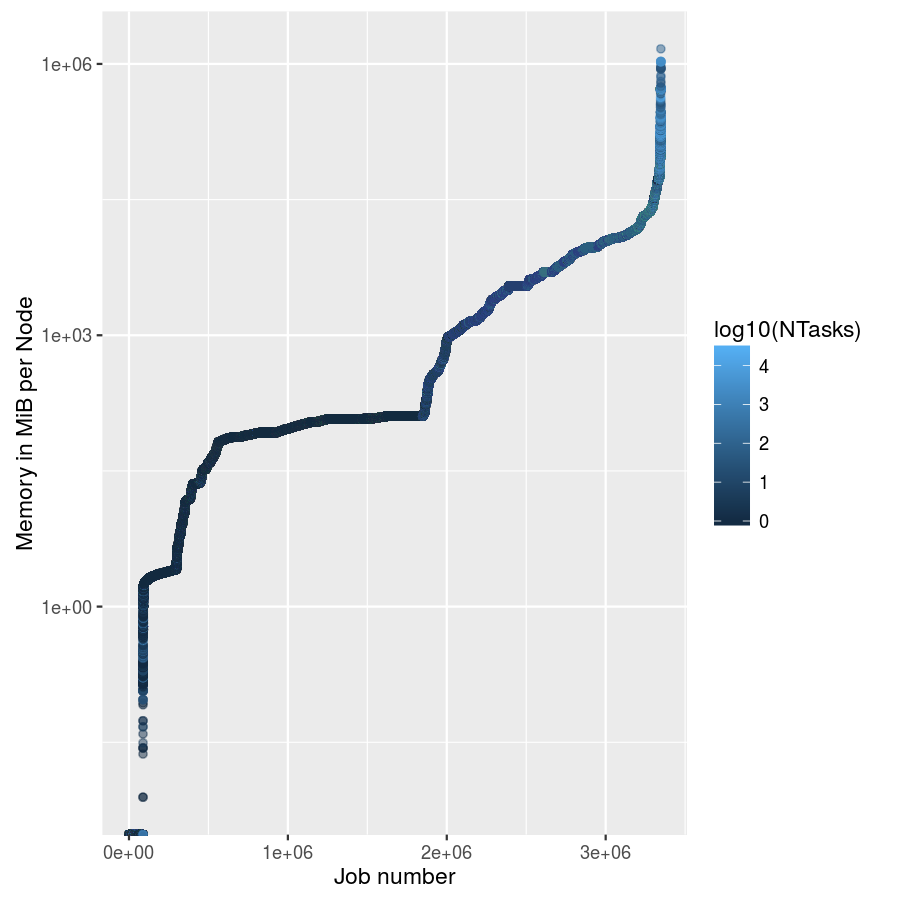
\includegraphics[width=\textwidth]{mem-stats/perNodeEstimateRSS}
\caption{RSS max}
\label{fig:rssMax}
\end{subfigure}
\begin{subfigure}[t]{0.49\textwidth}
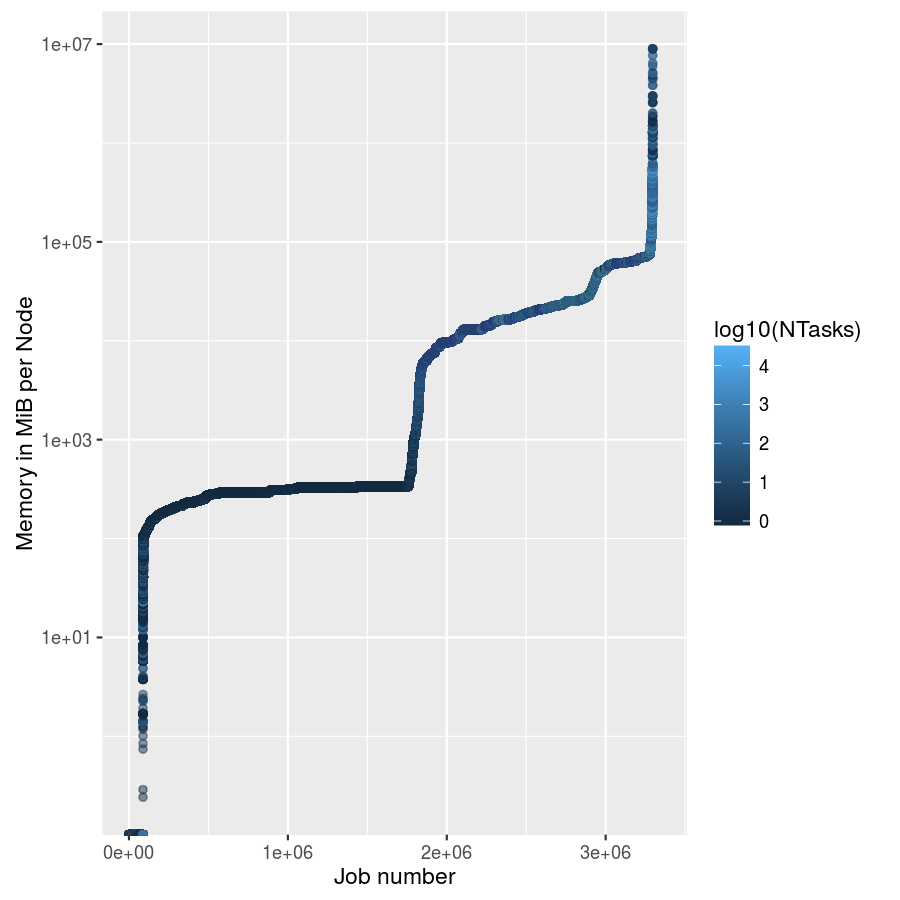
\includegraphics[width=\textwidth]{mem-stats/perNodeEstimateVM}
\caption{VM max}
\label{fig:vmMax}
\end{subfigure}

\caption{Job memory estimation per node}
\label{fig:job-memory}
\end{figure}





\begin{figure}
\begin{subfigure}[t]{0.49\textwidth}
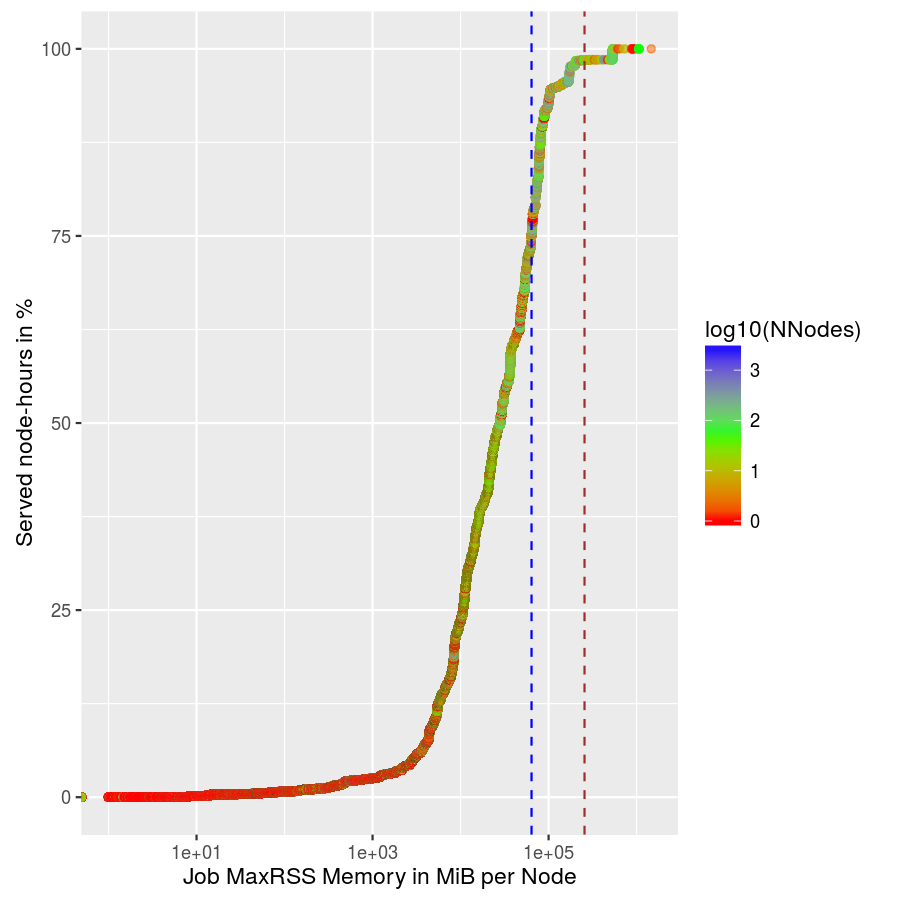
\includegraphics[width=\textwidth]{mem-stats/systemComputeFractionRSS}
\caption{RSS max}
\label{fig:fracRSSMax}
\end{subfigure}
\begin{subfigure}[t]{0.49\textwidth}
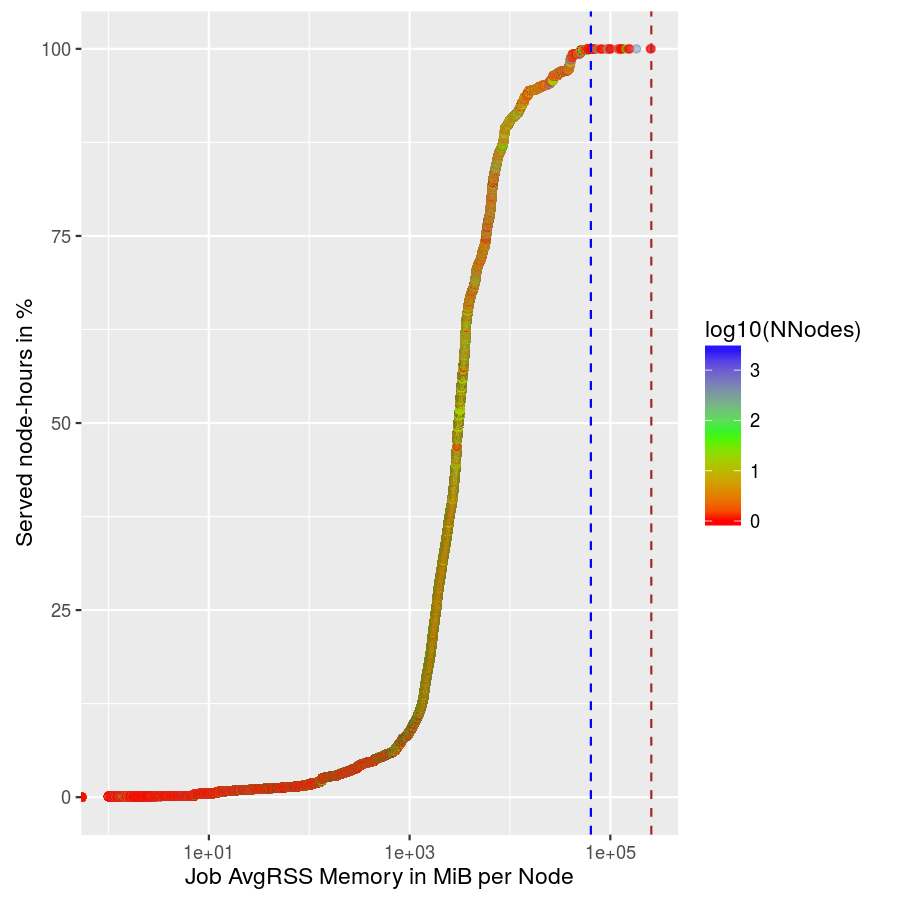
\includegraphics[width=\textwidth]{mem-stats/systemComputeFractionRSSAVE}
\caption{RSS average}
\label{fig:fracRSSAvg}
\end{subfigure}
\caption{Fraction of served node-hours vs. the estimated memory consumption}
\label{fig:fractionMemConsumed}
\end{figure}



\begin{table}

\begin{subtable}[t]{0.49\textwidth}
\begin{tabular}{r||r|r}
\% & RSS Ave & RSS max \\
\hline
usage & in MByte & in MByte \\
\hline
\hline
10 & 1,128 & 4,977 \\
25 & 1,836 & 10,625 \\
50 & 3,067 & 28,262 \\
75 & 5,793 & 63,925 \\
90 & 9,686 & 85,875 \\
92 & 12,585 & 96,282 \\
95 & 20,783 & 129,946 \\
96 & 26,952 & 170,357 \\
97 & 33,384 & 175,159 \\
98 & 39,621 & 201,648 \\
99 & 41,795 & 532,514 \\
\end{tabular}
\caption{Amount of memory utilized for the fraction of served node-hours}
\label{tbl:memUsageStats1}
\end{subtable}
\begin{subtable}[t]{0.49\textwidth}
\begin{tabular}{r||r|r}
Memory & RSS Ave & RSS max \\
\hline
in GiB & in usage \%   & in usage \%\\
\hline
\hline
1 & 8.8 & 2.5 \\
2 & 29.0 & 3.6 \\
4 & 66.7 & 7.1 \\
8 & 86.3 & 16.9 \\
16 & 94.4 & 36.8 \\
32 & 96.9 & 54.3 \\
64 & 100.0 & 75.1 \\
128 & 100.0 & 94.9 \\
256 & 100.0 & 98.5 \\
512 & 100.0 & 98.5 \\
1024 & 100.0 & 100.0 \\
\end{tabular}
\caption{Fraction of served node-hours that need a certain amount of memory}
\label{tbl:memUsageStats2}
\end{subtable}

\caption{Memory usage statistics of one year system usage computed from the jobs' data}
\label{tbl:memUsageStats}
\end{table}



\subsubsection{Example Scenario}

In this example scenario, we take the specifications from half of the current DKRZ system: 1400 nodes with 64 GByte, 110 nodes with 128 GByte, 12 Nodes with 256 GByte and one with 1 TByte = 107.7 TByte memory in total.
If we assume memory cost is 20\% of the compute nodes' costs\footnote{This assumption is motivated by the information reported from other supercomputers; also when looking at the current (2017) prices for a 32 GByte ECC DIMM (250 EUR): $107.7 \mbox{TByte} \cdot 250  EUR / 32 \mbox{GByte}  = 0.84 \mbox{M\, EUR}$.} and the first phase of the system cost was about half the full system, then 1.58 M EUR would be spent on memory.


If we had the same job mix as that described in \Cref{tbl:memUsageStats} with 64 GByte of memory in a node, we could satisfy 99.8\% of the system's node time for RSS average and 75.1\% for RSS max without falling below memory requirements.  With 32 GByte 96.7\% of the node hours can be served based on RSS average and 54.3\% based on RSS max.

Now assume we deploy only one type of node and dynamically provision memory beyond its size to the nodes as needed. If all jobs could be optimised to fit into 32 GByte memory, then we would have 1523 nodes with 32 GByte = 48.7 TByte memory (45.2\%). Based on the costs for the memory, 55\% could be saved (860 k EUR) - although this saving is not yet  balanced against the cost of the remote memory.

Since some of the applications require more memory, the dynamic provisioning will supply additional memory.
Assume we can dynamically allocate and deallocate the memory to fit between RSS max and RSS average based on the needs of the jobs. The question then would be: How much memory should be dynamically provisioned?
Certainly less than the difference between the normal system and a low memory system (difference is 59 TByte).
Say 10\% of this memory becomes dynamically provisionable = 6 TByte, an example configuration could be 
to equip nodes with the following combination of memory: 32 GByte for 100 nodes (6.5\% of nodes) + 96 GByte for 25 nodes (1.6\% of nodes) + 200 GByte for two nodes (0.1\% of nodes). (Note also that some of the local memory on nodes would be necessary as L4 cache.).

Again, assuming the same job mix, from the table, 3.1\% of node hours need an average RSS above 32\,GByte but below 64\,GByte. Thus, this combination could work in an optimistic scenario (equipping 6.5\% of nodes with the additional 32 GByte of memory). The costs of this additional 6 TByte for dynamic memory should not outweigh the saved money for the main memory to meet our goal of gaining an advantage over a traditional system with a fixed memory allocation.

Besides potential monetary gains of dynamic provisioning, there are several soft factors in favour for this approach:
\begin{itemize}
\item The dynamic provisioning allows to allocate and assign arbitrary memory sizes to a node. It becomes possible to operate on a node with 50 GByte of memory, for example.
\item The uniform node design reduces the conflicts in allocating nodes exclusively for jobs of a given size, and thus, potential unused nodes. This tends to increase the utilization of the overall cluster system.
\item Available pooled memory can be used for other purposes, e.g., a shared global scratch space and in-memory burst-buffer system.
This fast storage can be used to speedup post-processing of data and enables fast random access to extremely large data.
\end{itemize}

Such a scenario would lead to the following requirements for user workflows and system software:
\begin{itemize}
\item The dynamic memory must be easily provisionable to parallel jobs and potentially should be able to be freed to the pool when only needed for short runtime periods.
\item Support for the job scheduler is necessary to indicate usage of the external resource and prevent oversubscription during the runtime.
\item Users must understand the memory footprint of their applications.
The system could support this by providing tools to analyze and optimize the utilized memory footprint.
\end{itemize}

A disadvantage of the approach would be the increased complexity to analyse performance bottlenecks. Such performance bottlenecks may be intractable with current models which already have problems with data movement and communication, problems which would probably arise with dynamic memory allocation too --- although the amount and impact are difficult to assess a priori. For these, and other reasons, it may be non-trivial to fully analyse the cost-benefits, but the example shows there are potentials for cost savings which we intend to analyse further in the future.
%
%\comment{
%%%%%%%%%%%%%%%%%%%%%%%%%%%%%%%%%%%%%%%%%%%%%%%%%%%%%%%%%%%%%%%%%%%%%%%%%%%%%%%%
%%\subsection{Topo3: Site-global storage}
%
%%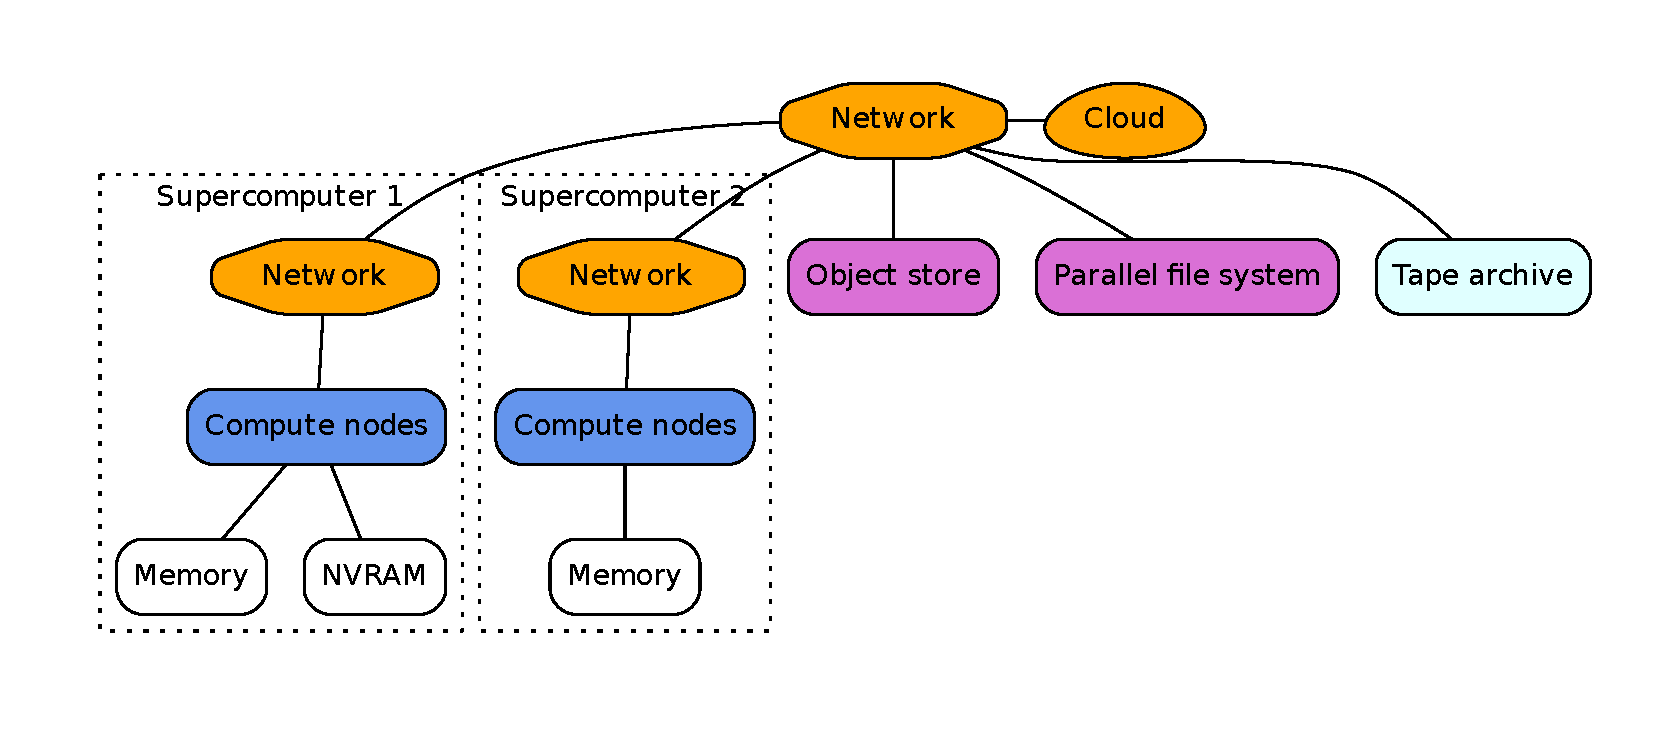
\includegraphics[width=\textwidth]{dot/topo-site-global-fs}
%
%a parallel application is started on supercomputer 1.
%We assume it is a large parallel application (more than 100 nodes):
%
%
%Is the storage bandwidth smaller than local NVRAM bandwidth?
%
%No: use the parallel file system (because it is faster).
%
%Yes:
%Checkpoints: store checkpoint in NVRAM, assign always the same nodes for compute to allow restart from the same node, every z checkpoints make copy to the parallel file system (asynchronously to prevent resilience problem).
%
%Iteration data: store (temporarily) in NVRAM, drain over network to parallel file system using QoS of the network (not disturbing the communication of the application).
%
%
%Do we know the further workflow? If people are not analyzing it for a while, we should probably put it on tape or object storage.
%We may apply in situ stuff?
%This also depends on the speed data is pumped in, as we must avoid to fill the NVRAM completely and stall the application to prevent data loss.
%If the object storage fits well the access pattern (performance will be good), we can store large chunks already on object storage.
%
%
%"running use-case 1"
%
%
%thus.. running simulations?!
%
%Where is it run?
%
%
%
%
%
%}



%%%%%%%%%%%%%%%%%%%%%%%%%%%%%%%%%%%%%%%%%%%%%%%%%%%%%%%%%%%%%%%%%%%%%%%%%%%%%%%
%%%%%%%%%%%%%%%%%%%%%%%%%%%%%%%%%%%%%%%%%%%%%%%%%%%%%%%%%%%%%%%%%%%%%%%%%%%%%%%
%%%%%%%%%%%%%%%%%%%%%%%%%%%%%%%%%%%%%%%%%%%%%%%%%%%%%%%%%%%%%%%%%%%%%%%%%%%%%%%
\newpage
\chapter{Refined Models}
\label{sec:refined models}

This  chapter describes how to model and simulate tape libraries using further refinements of concepts we have already introduced.

Currently tape archival systems are often loosely integrated into the HPC storage infrastructure, but in the near and exascale term, burst buffers and HTC computing will also require integration with the archive.  
Unfortunately, publicly available research on tape systems is scarce, leading to difficulties estimating and understanding costs, and in exploring new strategies and developing open software for tape systems. This is compounded by a lack
of affordable systems, and hence a lack of availability for experimentation outside of large organisations - where operational concerns may also restrict experimentation (on what is an integral part of the durability delivery of their organisations).
Lessening these problems by providing virtual storage silos should enable community-driven innovation and enable site operators to add features where they see fit while being able to verify strategies before deploying on production systems.

Here we develop different models for the individual components in tape systems. The models are then implemented in a prototype simulation using discrete event simulation..
\Cref{fig:tapesim model and software} illustrates some of the hardware and software components that are relevant to tape systems.


\begin{figure}
	\centering
	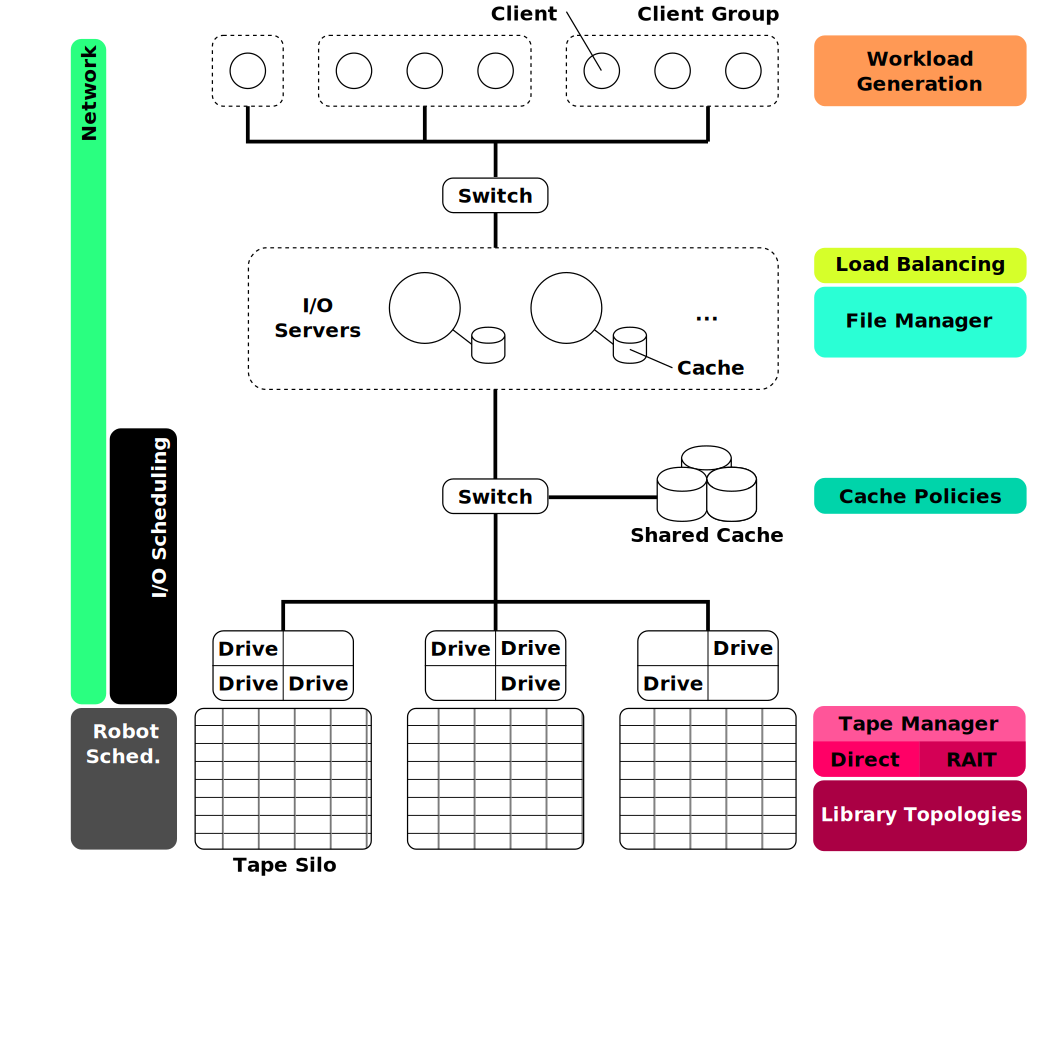
\includegraphics[width=0.75\textwidth]{tapesim/svg/model+software}
	\caption{Hardware and software components relevant to HSM and tape archives.}
	\label{fig:tapesim model and software}
\end{figure}


%%%%%%%%%%%%%%%%%%%%%%%%%%%%%%%%%%%%%%%%%%%%%%%%%%%%%%%%%%%%%%%%%%%%%%%%%%%%%%%
\section{Hardware Models}


One problem with computer systems is the complexity that unfolds because of the large number of possible combinations for hardware and software.
Modeling hardware is particular cumbersome because in the real world the performance of a device emerges as a result of the laws of physics, but for a virtual model the dynamics have to be understood and abstracted.
For standardized components it often is relatively easy to find a model that is adequately applicable for the whole class of of components.
Composite components, such as the library topologies turn out to be harder to generalize in a simple way than expected.
By mixing mostly 2D and a graph-based topology approaches good approximations of the library dynamics could be achieved.
Another problem occurs with proprietary designs for which detailed information is hard to find.
The same is true for benchmarks and a comprehensive catalogue of performance parameters.
The network is an integral part of hierarchical storage systems and can be used to model and simulate even low-level components and communication.

%%%%%%%%%%%%%%%%%%%%%%%%%%%%%%%%%%%%%%%%%%%%%%%%%%%%%%%%%%%%%%%%%%%%%%%%%%%%%%%
\subsection{Library Topology}

To model the library hardware we start with a course grained graph based topology
that connects individual components in combination with detailed models where
the graph based approach appears insufficient.
In some cases it can be easier and more efficient to choose a different model as is outlined in \Cref{sec:tapesim/2d topology}.

%%%%%%%%%%%%%%%%%%%%%%%%%%%%%%%%%%%%%%%%%%%%%%%%%%%%%%%%%%%%%%%%%%%%%%%%%%%%%%%
\subsection{Graph-based Model}
\label{sec:tape_simple_graph}

The coarse grained structure e.g. the way multiple library units are connected to form library complexes  with Pass-Through-Ports or Elevators is modeled using a graphs.
By allowing numeric values but also callbacks, the individual components can use sophisticated models underneath e.g. to account for their current state.
A vertex in the graph consequently is used for components and edges can be used to store distance or travel times from component to component.
In principle, the approach is very flexible and arbitrary accurate depending on the level of detail.
For highly detailed models, the approach can be tedious to configure and will be more expensive to compute.
For lower levels of detail, errors may quickly accumulate.
\Cref{fig:graph topology} illustrates the concept, and in this case mixes distances and times; this is just one of many ways to interpret edges and nodes in a graph based topology.
Usually an implementation will receive times and distances by invoking a method to allowing more detailed models to hide behind an edge or vertex.
In most systems, a robot can not pass another robot, the exact rulebook however should be handled in a separate component that prevents illegal actions.



\begin{figure}[b]
	\centering
	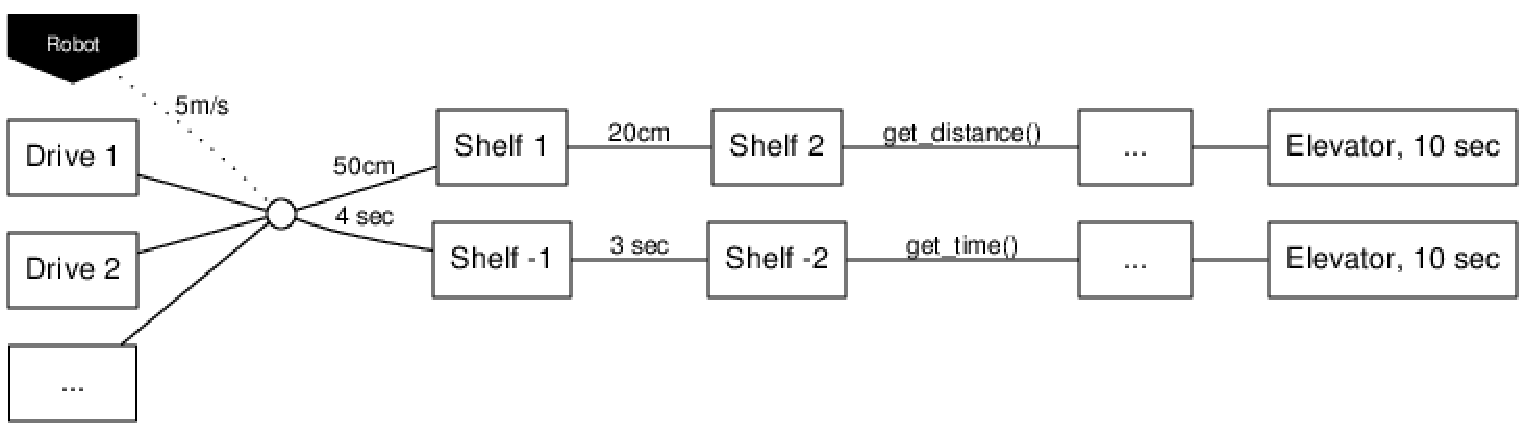
\includegraphics[width=0.8\linewidth]{tapesim/graphviz/graph-topology.pdf} % BNL changed extension
	\caption[Example: Graph Topology]{The graph based topology for coarse grained relationships including library complexes, Pass-Through-Ports and Elevators connecting multiple rails.}
	\label{fig:graph topology}
\end{figure}




This model is attractive as we can utilize algorithms that are familiar from
graph theory.
The task of serving a tape that sits in \texttt{Slots-2} to \texttt{Drive-1} becomes the problem of finding the shortest path. %which is easily achieved using, e.g.,  Dijkstra's Shortest Path in $\mathcal{O}(|E|+|V|log|V|)$ or more generally the A*-Algorithm.
%
%Only positive weights are assumed.
%Should negative weights be used for some reason one might consider using the Bellman-Ford algorithm instead.
%
%For large topologies with static distances, it may pay off to look into the \emph{all-pairs shortest path problem} to avoid needlessly recomputing the same paths over and over again.
For two vertexes $v_i$ and $v_j$ and edges $e_{v_i, v_j}$ the time $T_G$ to get from $v_i$ to $v_j$ calculates in principle as follows. With 
 $v_{robot}$ used to denote the maximum robot velocity, the time taken can be calculated:

\begin{equation}
\text{get\_time}(e_{v_i, v_j}\;\text{or}\;v) :=
\begin{cases*}
t & if $e_{v_i, v_j}$ or $v$ have time $t$ set \\
\frac{\text{get\_distance}(v_i, v_j)}{v_{robot}} & if $e$ but no time is set \\
0 & otherwise
\end{cases*}
\end{equation}

Hence

\begin{equation}
T_{G}(v_i, v_j) = \sum^{\text{shortest\_path}(v_0, v_1)}_{v_{i}, v_{j}}
\text{get\_time}(v_i) + \text{get\_time}(e_{v_i, v_j})
\end{equation}



\begin{figure} [h]
	\centering
	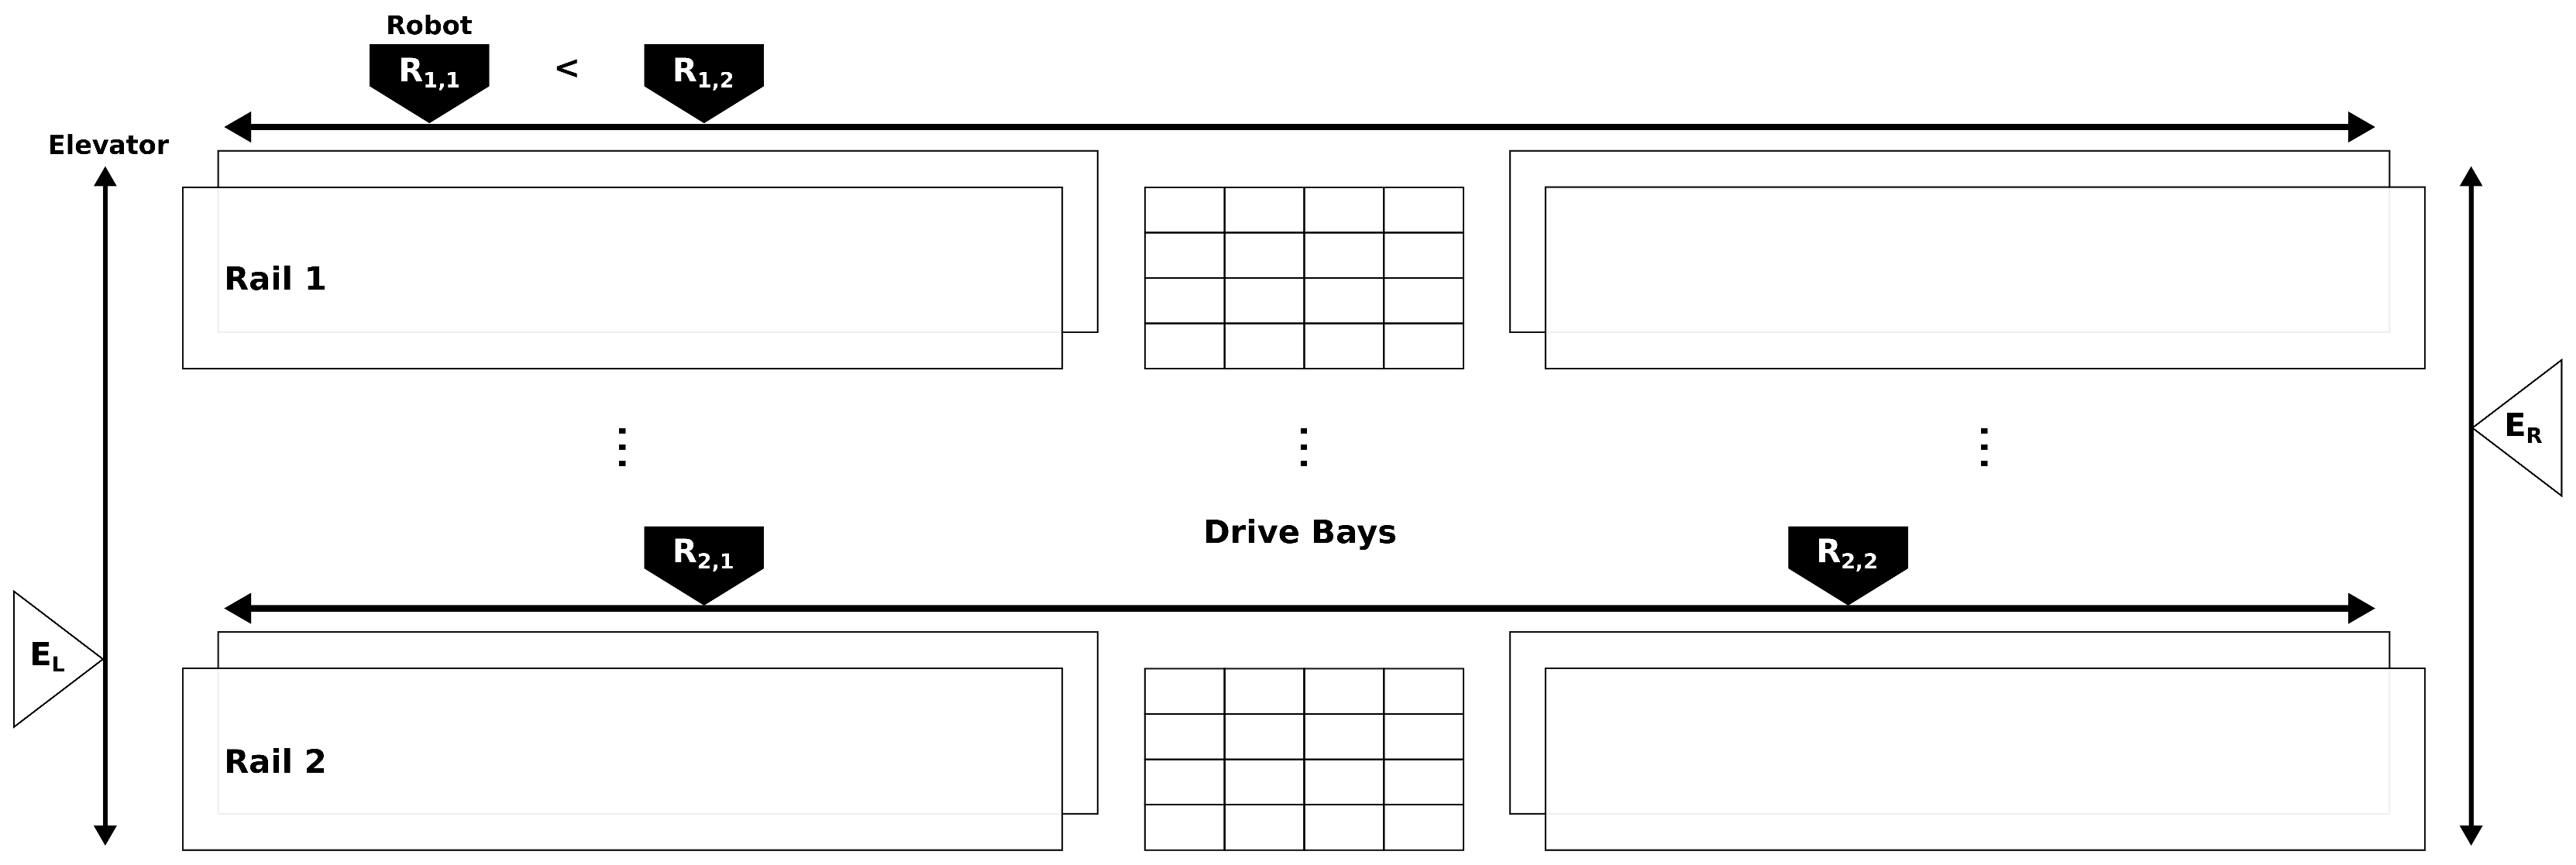
\includegraphics[width=\textwidth]{tapesim/svg/SL8500-minimal}
	\caption{An example 1D model for the component mapping and robot movements}
	\label{fig:sl8500}
\end{figure}




%%%%%%%%%%%%%%%%%%%%%%%%%%%%%%%%%%%%%%%%%%%%%%%%%%%%%%%%%%%%%%%%%%%%%%%%%%%%%%%
\subsection{2D Topology Model}
\label{sec:tapesim/2d topology}



\begin{figure}[h]
	\centering
	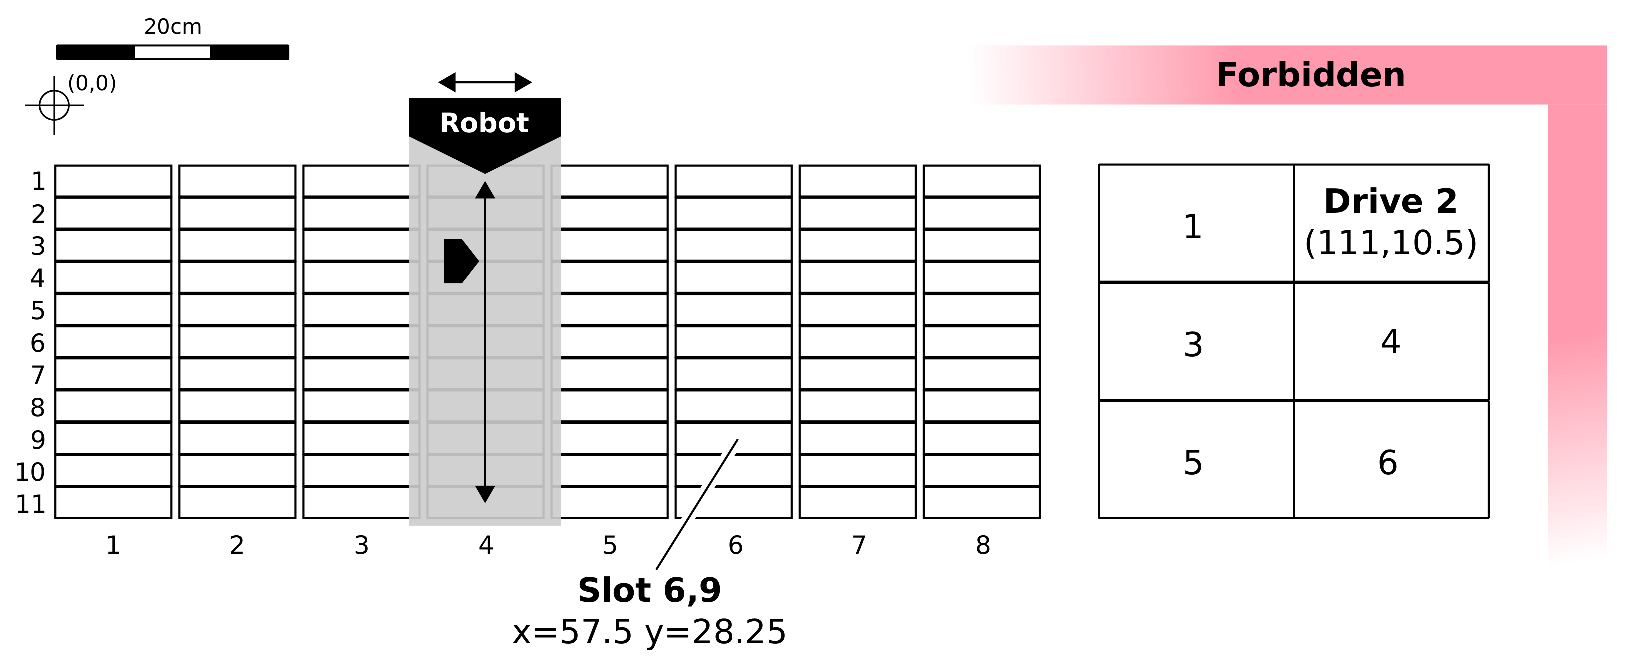
\includegraphics[width=\linewidth]{tapesim/svg/2d-model}
	\caption[Example: 2D Topology]{An example for a 2D topology model with a component mapping (in centimeter) coordinates and forbidden regions.}
	\label{fig:2D topology}
\end{figure}



Sometimes projecting complete robot libraries into a two dimensional representation yields very good approximations.
For the SL8500, this seems to be an efficient approach.
The reasoning is that many significant movements that can be performed by the robots or the library are anyway at most two dimensional.

A simplified 2D mapping of the components that are arranged in the U-shape is shown in \Cref{fig:sl8500}.
The robots move along on 1 dimension but the elevator permits movements in the orthogonal dimension.
Finding a path within a 2D model then becomes calculating the \emph{Euclidean-distance} between a number of points with a check if the robot is crossing a forbidden area or an obstacle, in which case
additional measures have to be taken.
Movements are usually decomposed into multiple linear movements, thus care must be taken when calculating distances and travel times.
\Cref{fig:2D topology} illustrates another way to representing a library in just two dimensional space but considers now distances between the different components (slots, robots and drives).

Logical components are resolved to coordinates by providing a mapping function for, e.g., slots and drives.
Mounting a tape placed in \texttt{Slot-6,9} to \texttt{Drive 2} requires visiting multiple coordinates.
Let  $T_{2D}(path)$ be the time it takes to traverse a $path \in \{(p_1, ..., p_n)\;|\;p_i \in (x,y); x,y \in \mathbb{R}\}$.
Assuming different robot velocities $v_x$ and $v_y$ for each axis, the total travel time may be defined by the sum of the time traversing between two points $T_{2D}(p_i, p_j)$ and possibly occurring work and wait times $T_{wait/work}$:

\begin{equation}
T_{2D}(p_j, p_i) = max \left( \frac{|p_{ix} - p_{jx}|}{v_{x}}, \frac{|p_{iy} - p_{jy}|}{v_{y}} \right) 
\end{equation}
\begin{equation}
T_{2D}(path) = \sum^{path}_{p_{i}, p_{j}}
T_{2D}(p_i, p_j) + T_{wait/work}
\end{equation}

An easing function $e(|p_{id} - p_{jd}|, v_{max})$ can to be used before taking the maximum should gradual robot acceleration be taken into account.
The exact times also depend on other robots, which reinforce the need for a component that guards the behaviour of the robot (as already noted in section\ref{sec:tape_simple_graph}).
2D topologies can greatly reduce the burden to model, even on first sight, complex systems as such as a single SL8500.
2D models are limited when library complexes are connected or more exotic parts (e.g., a high-density rotary drum) is used in the system.
In such cases, hybrid approaches that mix graph-based and 2D models are promising to achieve good approximations at reasonable effort.

%%%%%%%%%%%%%%%%%%%%%%%%%%%%%%%%%%%%%%%%%%%%%%%%%%%%%%%%%%%%%%%%%%%%%%%%%%%%%%%
\section{Software Models}

Hardware devices and subsystems such as the library topology and the network are controlled by software and subject to complex workloads.  For a proof of concept prototype it often seemed sufficient to turn to ``naive" implementations, but
with a modular model such as the one constructed here,  more sophisticated algorithms can be integrated into the virtual software stack.

In particular, to stress the virtual tape library, a request object can be instantiated and submitted to the simulation.
In addition to explicit submission it possible to register event providers to the simulation.
As the simulation proceeds event providers are polled for future events until they indicate they have been drained.

With this formalism, it is possible to create a workload provider to create requests on the fly according to a script, a probability distribution, or a trace file. In a similar fashion it would be possible to generate service workloads or component failures.

We have implemented support for two important components: workload generation and resource scheduling, covered in \Cref{sec:refined/workloads} and \Cref{sec:refined/scheduling} respectively. 

\subsection{Workload Generation}
\label{sec:refined/workloads}

We here concentrate on two main workload types: reads and writes induced by clients. For the experiments in this section workload traces were used, which is convenient to mimic real workloads although it would have been 
  possible to generate workloads randomly or based on probabilities estimated
  for future workloads.
  
In this model using workload provider, it is also possible implementing simple workload kernels as Python scripts which are registered with the simulation.
\Cref{fig:request handling} illustrates the life cycle of writes (a) and reads (b).

\paragraph{Write:}
A write request is send by a client to an I/O server, which writes it to a shared cache.
For the client the request is already served at this point.
In a second phase an I/O server issues the actual write onto a tape.

\paragraph{Read:}
A client issues read requests to an I/O server.
The I/O server checks if the file is in the shared cache.
If that is the case, the I/O server can immedietly start serving the request.
If the file is not already cached the library has to receive and mount the tape first.

\begin{figure} [h]
	\centering
	\begin{subfigure}[t]{0.47\textwidth}
		\centering
		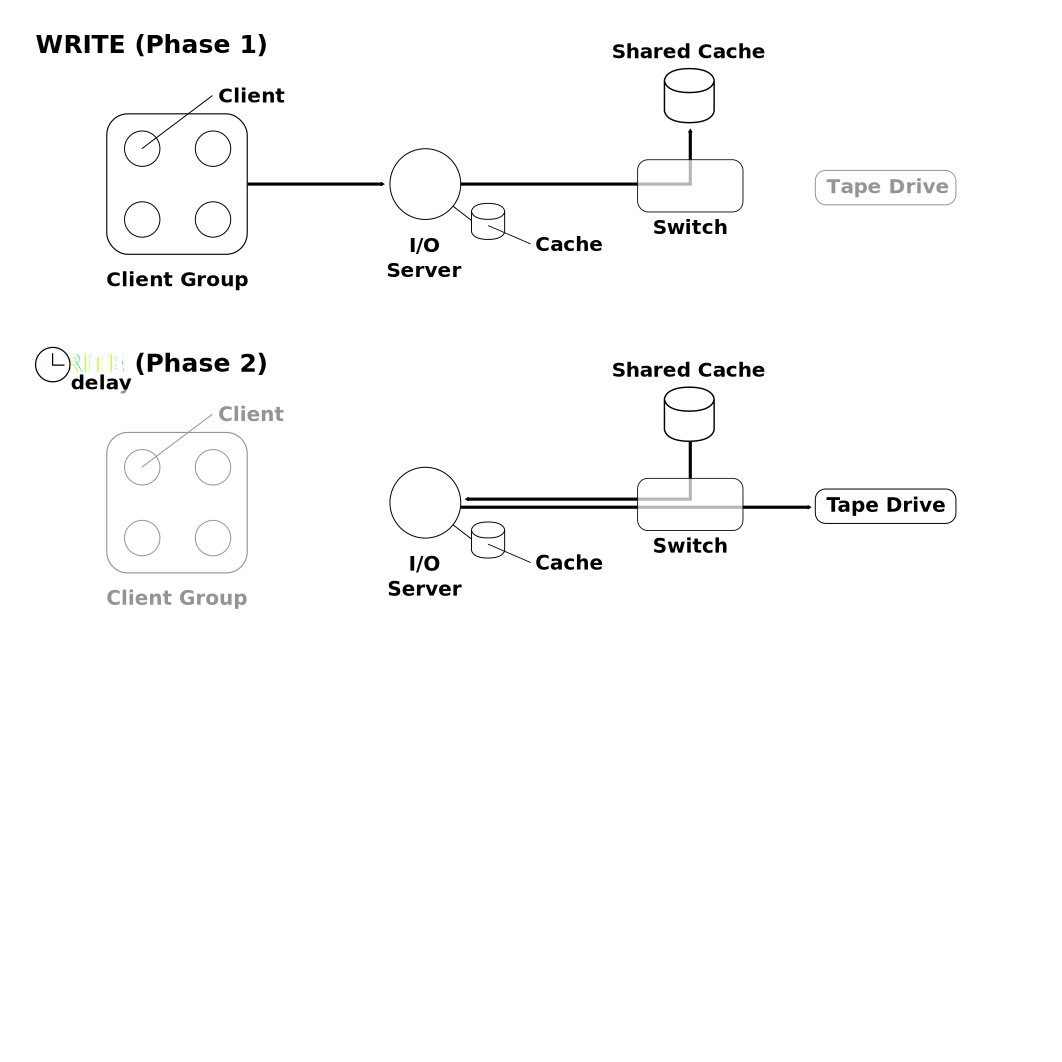
\includegraphics[width=\linewidth]{tapesim/svg/request_WRITE}

		\vspace{0.6em}

		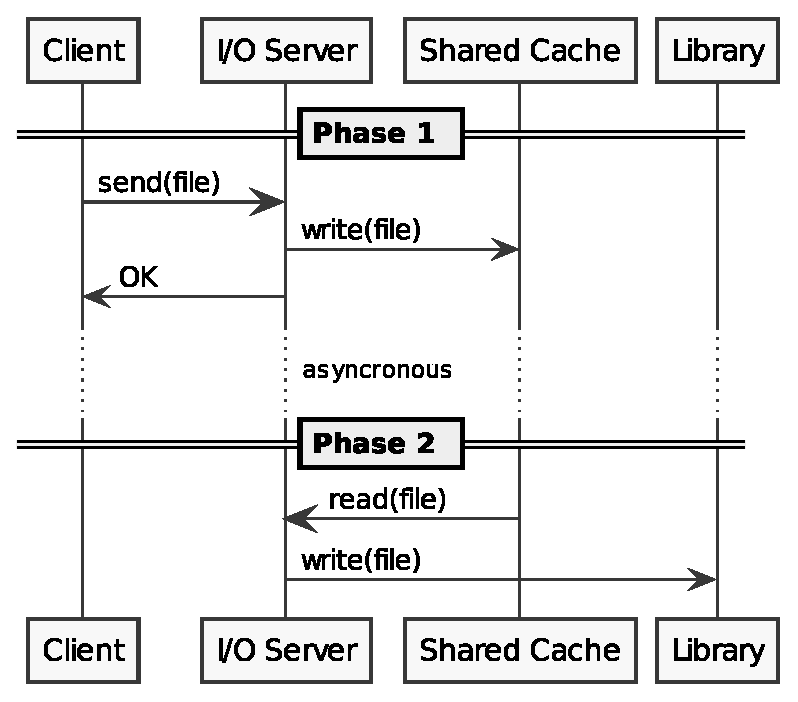
\includegraphics[width=0.93\linewidth]{tapesim/plantuml/activity_write-fix}
		\caption{Life-cycle Write}
	\end{subfigure}
	\begin{subfigure}[t]{0.47\textwidth}
		\centering
		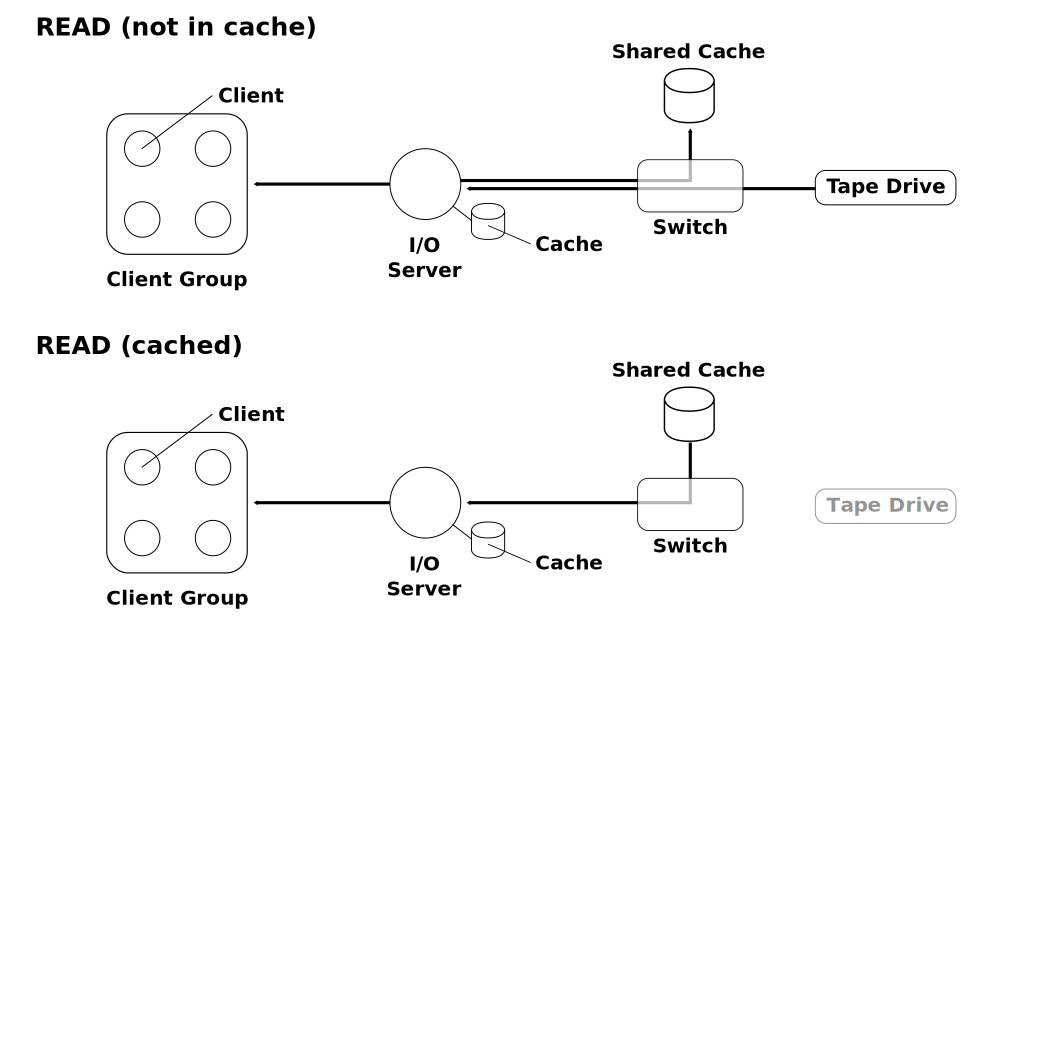
\includegraphics[width=\linewidth]{tapesim/svg/request_READ}

		\vspace{0.5em}

		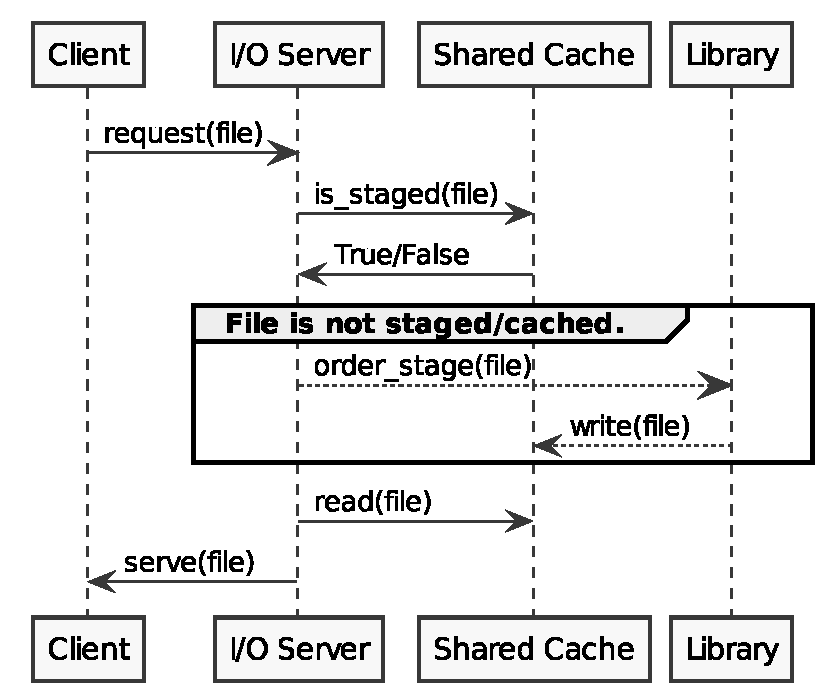
\includegraphics[width=0.96\linewidth]{tapesim/plantuml/activity_read}

		\caption{Life-cycle Read}
	\end{subfigure}

	\caption{Handling of read and write like requests for the HSM tape system.}
	\label{fig:request handling}
\end{figure}

\subsection{Scheduling}
\label{sec:refined/scheduling}

To process the requests it is necessary to implement at least naive scheduling components.
\Cref{fig:chained request queues} illustrates the various queues and resources that are involved in a HSM tape system.
Requests arrive and are collected in an incoming queue.
A scheduling components assigns work to available I/O nodes and en-queues the request for subsequent resources.
An uncached read requests and data written only to the cache first requires a tape drive before performing tape I/O, which in turn has to wait for a robot to deliver and mount a tape.
Data incoming from clients or tapes requires a network allocation as well as an I/O allocation.
The shared cache has to distinguish between dirty data and data which can be displaced directly as space is required to handle incoming request.

\begin{figure} [h]
	\centering
	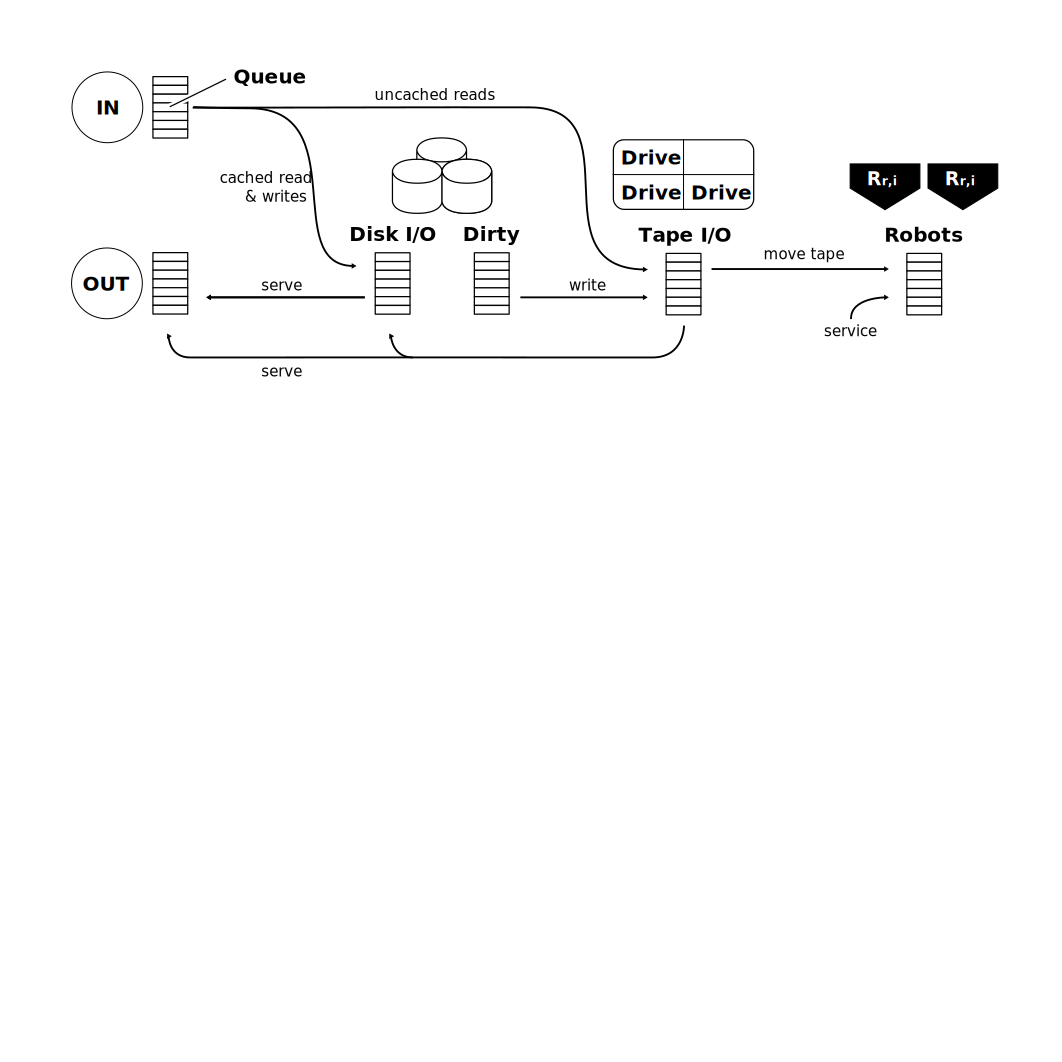
\includegraphics[width=0.8\textwidth]{tapesim/svg/chained-request-queues}
	\caption{Key queues and resources in a cache fronted tape system.}
	\label{fig:chained request queues}
\end{figure}

%%%%%%%%%%%%%%%%%%%%%%%%%%%%%%%%%%%%%%%%%%%%%%%%%%%%%%%%%%%%%%%%%%%%%%%%%%%%%%%

\section{Comparing actual System Monitoring to Simulation}


For the evaluation of the simulator, workload traces of FTP traffic covering
roughly a month of FTP traffic on the production archive of DKRZ were used
to stress the virtual system. Different metrics available through the original
monitoring system were collected within the simulation to reproduce the plots
for comparison (see Figure \ref{fig:monitoring-real}
%and Figure \ref{fig:monitoring-virtual}
).
The used trace in this case was chosen to also see how the virtual system recovers
from a maintenance phase.


\begin{figure}
	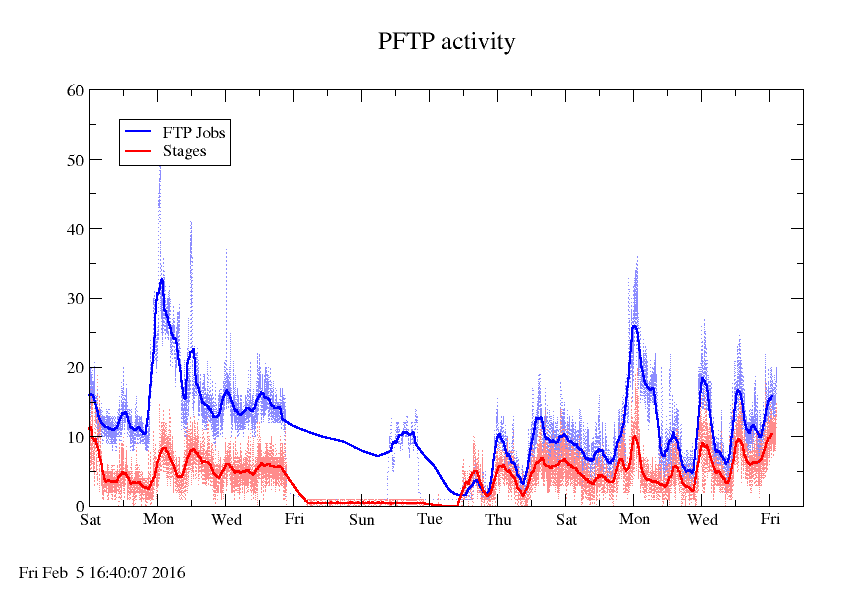
\includegraphics[width=0.49\linewidth]{tapesim/manual/observed_hpss-rtmu_stage-201xxx.png}
	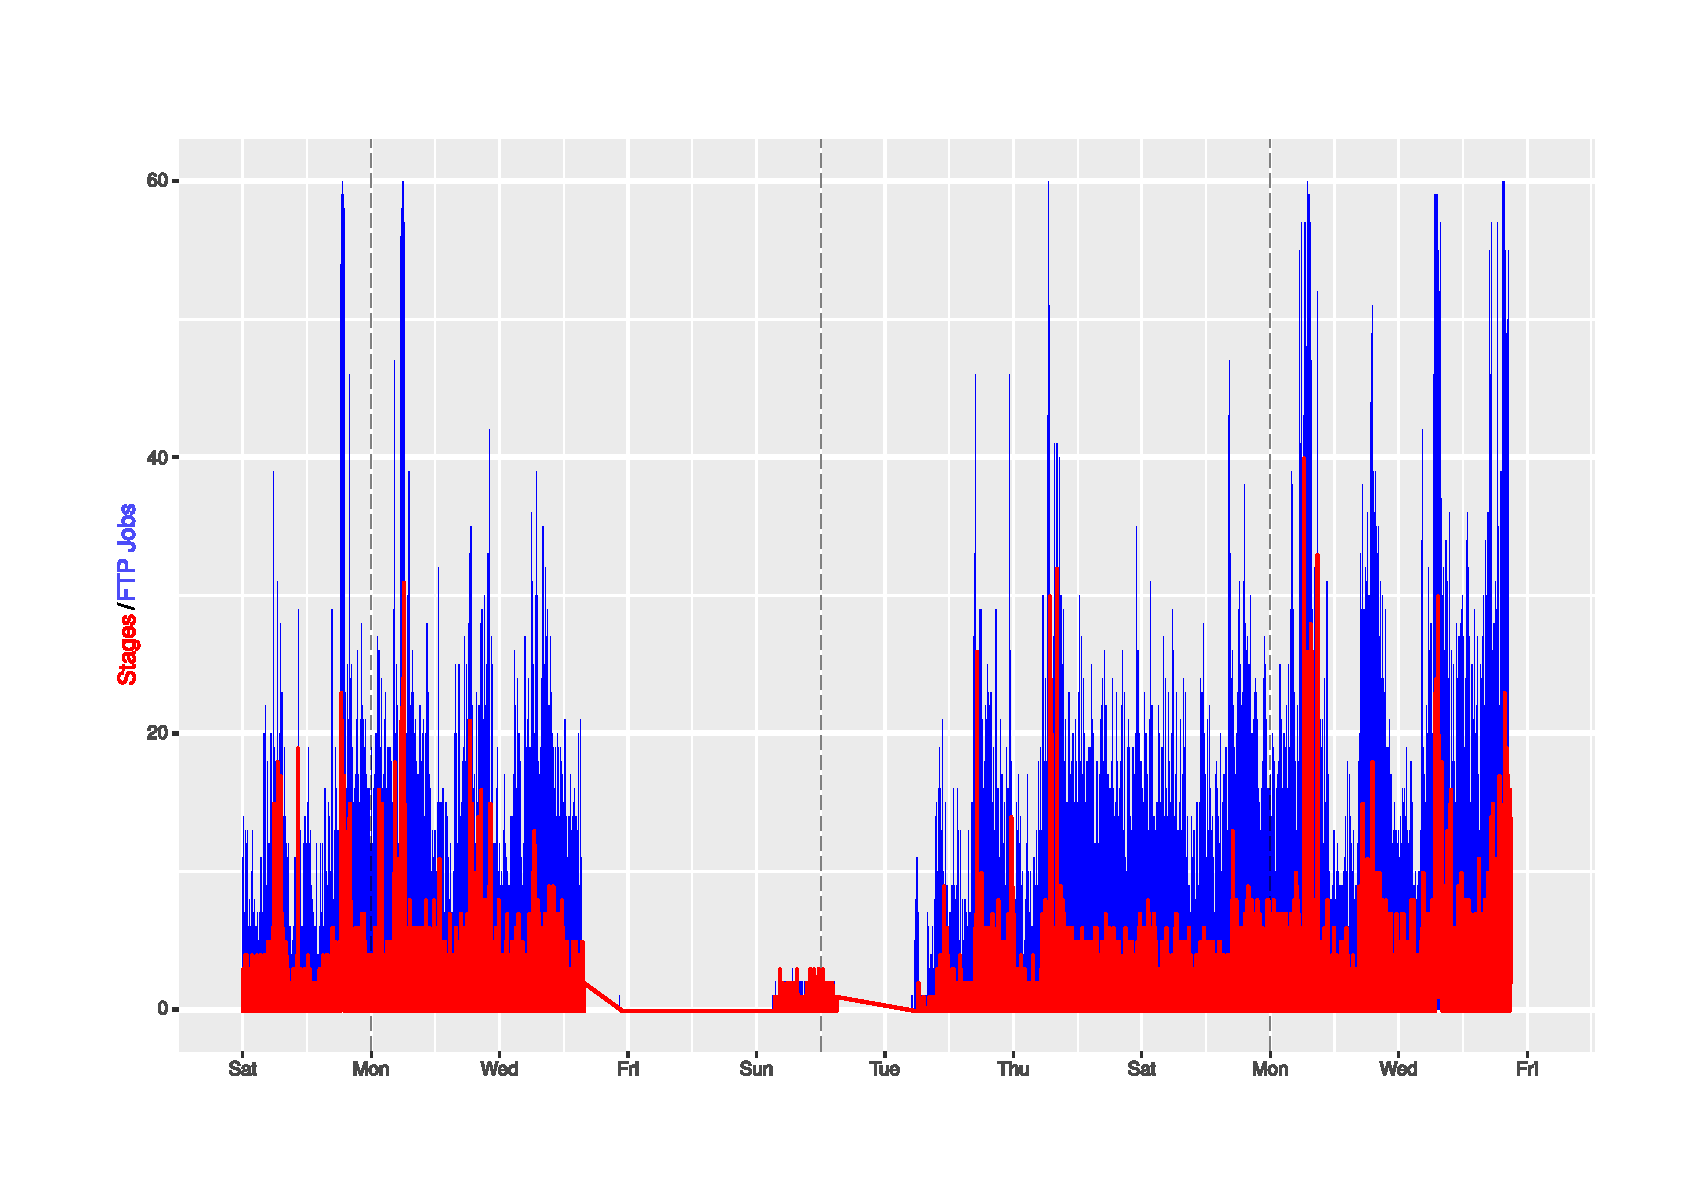
\includegraphics[width=0.49\linewidth]{tapesim/manual/plot_verification-merged-size-match.pdf}
	\caption{FTP activity and the number of stages observed by the monitoring of a real system (left) compared to a simulation run (right).}
	\label{fig:monitoring-real}
\end{figure}


\subsection{Use-Case: Drive Count Variation and Quality of Service}

By varying the number of drives (e.g. 30, 45, 60) we can verify if changes with
expectable outcome are consistent with the simulation outcome. With more of
these tests confidence in the simulation results increases and more experiments
with more elaborate strategies can be pursued.
A common question when dealing with tape systems concerns the number of tape
drives to be used. For the use-case on drive count variation Figure \ref{fig:stages-waits}
shows how the wait times and number of stages change depending on the configuration.


\begin{figure}
	\centering
	\begin{subfigure}[t]{\textwidth}
		\caption{30 Drives}
		\includegraphics[width=0.49\linewidth]{tapesim/data/thesis/30-drives-all/generated_plots/plot_snapshot-stages-timeline-limited.pdf}
		\includegraphics[width=0.49\linewidth]{tapesim/data/thesis/30-drives-all/generated_plots/plot_snapshot-waiting-timeline-limited.pdf}
	\end{subfigure}
	\begin{subfigure}[t]{\textwidth}
		\caption{45 Drives}
		\includegraphics[width=0.49\linewidth]{tapesim/data/thesis/45-drives-all/generated_plots/plot_snapshot-stages-timeline-limited.pdf}
		\includegraphics[width=0.49\linewidth]{tapesim/data/thesis/45-drives-all/generated_plots/plot_snapshot-waiting-timeline-limited.pdf}
	\end{subfigure}
	\begin{subfigure}[t]{\textwidth}
		\caption{60 Drives}
		\includegraphics[width=0.49\linewidth]{tapesim/data/thesis/60-drives-all/generated_plots/plot_snapshot-stages-timeline-limited.pdf}
		\includegraphics[width=0.49\linewidth]{tapesim/data/thesis/60-drives-all/generated_plots/plot_snapshot-waiting-timeline-limited.pdf}
	\end{subfigure}

	\caption{The number of stages (left) and the wait-time (right) for different drive counts.}
	\label{fig:stages-waits}
\end{figure}






%\begin{figure}
%	\centering
%	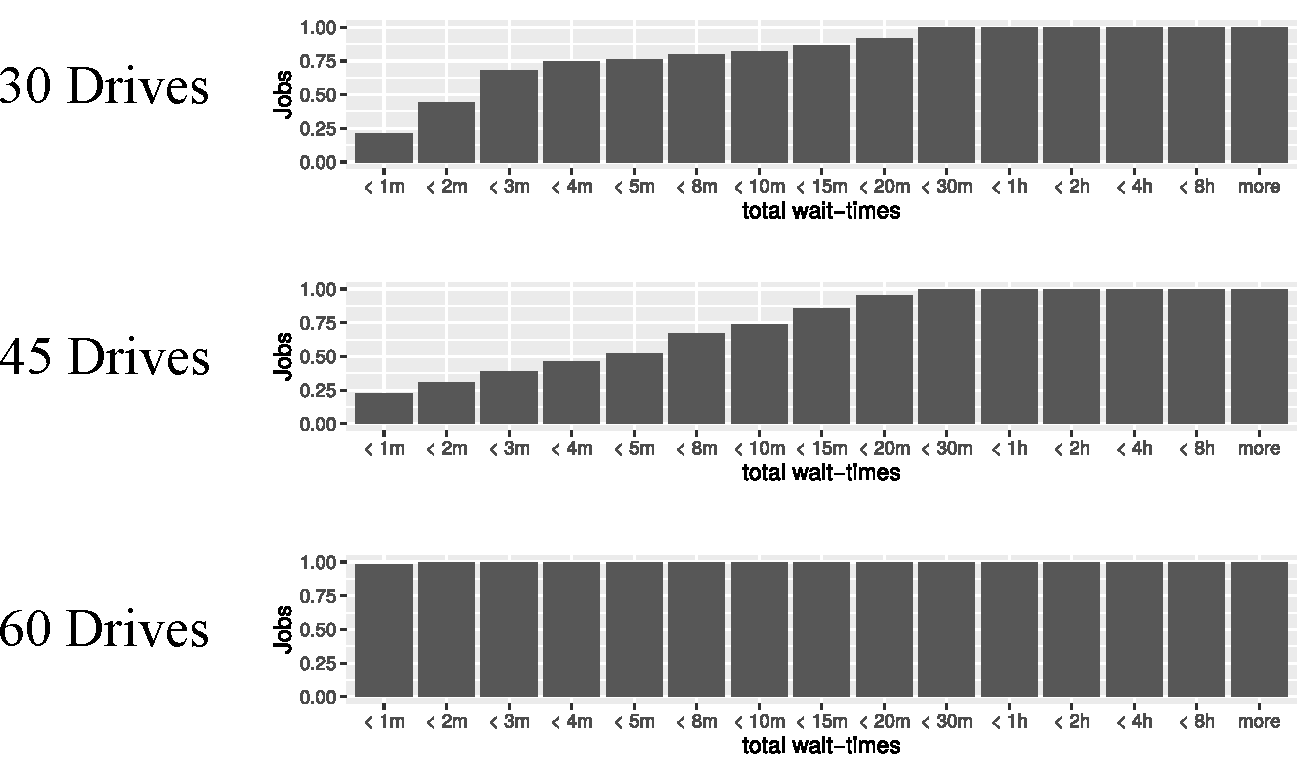
\includegraphics[width=0.5\linewidth]{tapesim/manual/plot_wait-times-cum-ALL.pdf}
%	\caption{}
%	\label{fig:qos}
%\end{figure}



\section{Summary for Refined Modeling}

This case study provided insight into the simulation of large scale hierarchical storage systems, but also shows that turning to refined models with the current state of the art of available tools is a daunting exercise.
Simulators are lacking ready to be used abstractions for high-level data centre components, as well as the necessary data describing post-processing/real-time workflows that would allow one to inspect system behaviour for comparison with the monitoring tools available with physical systems.

Refined models prove to require a large initial effort and meticulous knowledge about the individual hardware components and their interactions during the development of the simulator.  This information needs to be supplemented by at least naive drivers and scheduling algorithms for all important parts of the software stack. 
Finally, researchers (both model developers and model users) need to specify the performance metrics/characteristics they need or would like to know about and also the workloads they would like to use to stress the virtual system to evaluate run time behaviour. In the case of cost analysis, this also should include power consumption and initial hardware costs.

It would be beneficial, if vendors would provide testable models of their components such that simulation could validate the expected behaviour for performance as resilience as intended by the vendor\footnote{This transition is already happening in the manufacturing business; some companies force their suppliers to ship models and CAD files to simplify the construction of larger systems.}.

The case study also shows that while a broad range of problems needs to be addressed in a refined modeling approach, the resulting runtime performance can approximate the system performance of actual observed systems.
As the system complexity seems destined to increase, the simulation of storage systems promises to deliver a better understanding and promote research for new domain specific architectures. This will become ever more important as vendors 
 often lack the incentive to investigate specialized solutions, and it falls to data centres and research institutes to evaluate how hardware and software could be assembled to meet their bespoke requirements.




%%%%%%%%%%%%%%%%%%%%%%%%%%%%%%%%%%%%%%%%%%%%%%%%%%%%%%%%%%%%%%%%%%%%%%%%%%%%%%%
%%%%%%%%%%%%%%%%%%%%%%%%%%%%%%%%%%%%%%%%%%%%%%%%%%%%%%%%%%%%%%%%%%%%%%%%%%%%%%%
%%%%%%%%%%%%%%%%%%%%%%%%%%%%%%%%%%%%%%%%%%%%%%%%%%%%%%%%%%%%%%%%%%%%%%%%%%%%%%%

\chapter{Conclusion}
\label{sec:conclusion}


%%%%%%%%%%%%%%%%%%%%%%%%%%%%%%%%%%%%%%%%%%%%%%%%%%%%%%%%%%%%%%%%%%%%%%%%%%%%%%%
\section{Summary}

The report discusses the important issue of data handling for the weather and climate community.   It is necessary to understand both the short and long-term costs for the workloads associated with running, storing, and utilising data, in order to make educated procurements which deliver the best possible storage and performance with limited budgets - in the presence of rising demand for data storage and utilisation.

\Cref{sec:introduction} introduced the background motivation for this work: performance issues and costs associated with data handling are consuming more time and money of ever growing portions of the environmental science community. As these costs grow, the importance of making cost effective procurements which meet performance expectations grow - and as noted in \Cref{sec:refined models}, it is not easy to access existing research, benchmarks, or real systems for data (or  experiment).

% Data centre requirements:
%

\Cref{sec:dc_model} covered the functional responsibilities of data centres and how they provide researchers with virtual working environments to conduct their research.
To provide the required services, data centres have overcome many technical challenges.
As data centres provide a data lake of valuable data, the research community demands means for efficient I/O, data discovery and access tools that regularly exceed the capabilities of current technologies.


% Related Work:
%
In \Cref{sec:related work}, relevant related work that pushes these limits is collected and discussed.
The report looked at the evolution of data centres and various approaches concerned with data access that have been used in scientific contexts.
We covered the trends in both climate and weather research as well as the development of storage technologies and, in particular, discussed the performance divergence of compute vs. storage.
In this context, we also reviewed cloud technologies that have the potential to change the scientific computing landscape.
The report also looked at the data centre perspective and vendor perceptions on the cost developments of disks, NAND and tape.
It becomes obvious that a lot of potential still can be found in alternative software architectures for operating clusters and the workload programming.
But a fundamental field of research remains to find convenience and efficient paradigms to program upcoming systems.


%data centre evolution
%	general
%
%	cloud srvice providesr
%
%	data acces and transfer
%		hdf5
%
%trends for storage technologies
%	performance
%	cost
%	Disk, Nand, Tape
%
%	HPSS RAIT
%
%	NAND technology roudmap
%
%	network
%
%
%climate and weather developments
%	exponential data growth

%
%	data distribution
%
%	cloud
%
%	energy efficient
%
%
%software paradigms
%	LFS
%	Big data
%	erasure codings
%
%	cloud
%
%	improvements ot checkpoint restart
%
%	namespace consolidation PGAS
%
%
%Data transfer area



% Cost modeling:
%

In \Cref{sec:modeling}, the report then describes high-level considerations for costs, performance and resilience considerations.
A hierarchical graph-based approach is proposed allowing us to specify component and system characteristics and costs and visualize them.
This also allows to add or remove complexity and detail as becomes necessary and open the possibility for automation.
In the model, we also look at the core components that are usually found in data centres.
Starting with the smallest components such as hard drives, that provide little tuning opportunities, the report moves on to discuss how derive the emergent performance and cost of small subsystems like individual compute and I/O nodes as well as of  larger subsystems like the network or a parallel file system.
Separately from on site equipment considerations for the cloud are discussed.


%unit components procured more or less as is.. only require to update with specs provided
%for sub systems recalculate based on:
%
%considerations for core tehcnologies
%dependency to compute
%I/O nodes
%and specific storage subsystems.
%
%Object Stores
%Storage class media
%
%Tape
%
%cloud


% Evaluation:
%

In \Cref{sec:evaluation}, we provided the characteristics for costs and performance of currently deployed systems.
Starting from these systems as baseline, we explored changes to the system and the impact on cost, power consumption and performance applying coarse grained models.
The discussed scenarios do not aim to quantify the costs accurately but instead provide a qualitative perspective on the chances various modifications of the system may imply.
In that sense, they serve as blueprints for subsequent scenarios.
For example, we discussed reducing the storage budget in favor of compute resources -- with the goal to not decrease scientific productivity, and conclude that this requires more intelligent scheduling and staging mechanisms.
Researchers would likely need to drastically change their applications as well as their workflows.
The report shows that the cost developments for the technologies are an important but unknown factor and that it is therefore advisable to push for more flexible infrastructures to make the integration of new technologies easier.
One such technology, NVRAM, might shape future data centres radically, but the cost-benefits of this technology is difficult to quantify as the cost-prognostics of this technology does not exist.
Another factor maybe an increased integration of cloud like service.
Centralizing some resources such as (pooled) memory, introduces some opportunity, but the benefits are difficult to judge right now as we do not have all the data for the impact on the workload available right now.
Still, the abstract models shed light on the available design space.


% Refined Models.
%
While the high-level models can show certain cases for which a certain technology is useful, it cannot quantify the benefit for individual workloads as the dimension of time and the workload characteristics is abstracted.
An approach for more detailed models is showcased in \Cref{sec:refined models}.
Using discrete event simulation, it is possible to account for the workload behavior of a system.
In particular, we introduced a simulation for hierarchical storage systems that integrate tape libraries and online storage.
The case study demonstrates the overhead associated with fine grained models but also shows that it is possible to approximate the observed behavior in the actual system monitoring.
It is then shown that by varying the configuration, we can make forecasts for impacts on the quality of service of an alternative system configuration.

%%%%%%%%%%%%%%%%%%%%%%%%%%%%%%%%%%%%%%%%%%%%%%%%%%%%%%%%%%%%%%%%%%%%%%%%%%%%%%%
\section{Future Work}
\label{further-work}

This report has added to the understandings of costs and performance related to storage infrastructure, beginning with discussions of requirements, and moving through coarse and refined models. However, it leaves many avenues as yet unexplored, and the technology landscape is changing rapidly --- there is much yet do, including:
\begin{itemize}
	\item Refine models: include additional relevant parameters and consolidate models into interactive tools to directly support discussions of architecture changes and their impact.
	For example, for our high-level scenarios one could enter the data centre characteristics and explore the changes on various characteristics with the changes in architecture.
	\item Cataloging: Build a catalog of metrics for the components including failure rates and cost.
	This is a community effort, because the wide range of products is obviously out of scope of a single organization.
	\item Testing. The models have to be tested and improved along with actual procurement, to iteratively derive a toolchain to aid the decision making.
	We have already seen many opportunities for abstractions while compiling this report.
	\item Gathering more workload data: Refined models are promising and, given increasing hardware options, an imperative to pursue.
	However, they require that centres have, and share, detailed understandings of user workloads and how they change in the future.
	%The overhead to perform simulations can reduced significantly by developing with reuseable frameworks in mind.
\end{itemize}

\appendix
\chapter{Definitions}
\label{sec:definitions}
\vspace{2em}

This appendix collects and introduces important concepts and components as they find application in weather and climate related compute and storage infrastructures.

%hardware: disks, disk enclosures, servers, network,  ... tape, tape drive, tape library ... RAID,  .. etc
%software: parallel file system, object store, libraries, parts of the OS

\section{Data centre}

\paragraph{Data centre:}
A special purpose facility to accommodate compute, network and storage hardware to provide IT services from a centralized place under efficient and secure operation.
Most data centres arrange hardware to be grouped when contributing to a similar purpose.
One will commonly find buildings, floors or rooms partitioned into areas dedicated for compute resources, temporary storage (usually disk based but increasingly NAND) and storage for archival (e.g., tape libraries).
Modern data centres often have special requirements such as heavy duty structural analysis of the building, (emergency) power supply, ventilation and increasingly plumbing arrangements for liquid-based cooling infrastructure.
For many data centres also additional security systems and access control are a factor.

Therefore, the costs for constructing and maintaining the infrastructure for a data centre are considerable.
One of the options for implementing a data centre is to co-locate it (renting space in a shared data centre), or have it hosted by a third party.  This obviously reduces the costs (at least the CAPEX) of the initial procurement of the data centre.

\paragraph{Public Data centres}

A public data centre, is funded my the government, i.e., tax money of the citizens.
It usually serves scientific services, i.e., research or is highly relevant such as a data centre dedicated to compute the weather forecast.

\paragraph{Commercial Data centres and Services}

Commercial cloud service providers (CSPs) can provide services very easily at the lower end of the scale; higher end services (with large data volumes and/or large scale CPU requirements, or requiring specialized services) tend to require specialized negotiations with the CSP, for example on costs and availability of resources.  Possibly, a separate SLA is required.

As discussed in section~\Cref{sec:cloud}, the use of CSPs is useful for precisely what clouds were designed for --- namely, on-demand resources.  For example, a common usage pattern seen in research data centres is a spike in demand from a particular user community the week before their conference, and a cloud service is ideal for that type of usage pattern.  It follows that data centre interfaces and protocols should be designed in a way to allow for hybrid models, data centre/cloud.  This, in turn, would give end users of the service the ability to bring ``their own'' compute in the cloud.

Another commercial option is to rent a container data centre --- the physical kind, with computing nodes inside the container; it is put in the car park and powered up and networked.  There is no maintenance on it directly; once enough nodes have died, the container is drained of data, powered down, and replaced.

In a typical data centre we can find the following components:

\paragraph{Compute nodes:}
The most powerful compute systems today are so called cluster computers.
Many smaller compute units, called nodes are connected in a computer network to collectively run a simulation, perform data analysis or create visualizations.
Depending on the task, compute nodes can create massive amounts of data.
Climate applications are periodically stored to more permanent storage systems as computer failures are power outages result in loss of any data residing in the nodes memory.


\paragraph{Network:}
The network is used to connect the compute nodes as well as other subsystems, in particular storage infrastructure.
It is common to find high-speed and low-latency interconnects such as Infiniband to be used to connect individual nodes while
more affordable network technologies are used to communicate with the other subsystems. Storage systems are often attached
using FibreChannel protocol. Low-cost Ethernet technologies also has a stable appearance, as the standard keeps innovating.
Lately Intel is promoting its proprietary Omnipath interconnect. As a response, the Gen-Z consortium\footnote{\url{http://genzconsortium.org/}} formed, which is a joint
effort to develop a open, non-proprietary and royalty free standard.

\paragraph{Storage layers}
A typical I/O path for applications running in data centres is shown in \Cref{tab:storage layers}.
Applications run on compute nodes and perform I/O operations that traverse an internal network,
which may use additional gateway nodes in the I/O path to process the data.
Finally, I/O requests are processed by I/O servers and data is stored on block devices connected via Storage Area Networks (SAN) or directly connected to the I/O servers.

\begin{table}[]
	\small
	\centering

	\bgroup
	\def\arraystretch{1.5}%  1 is the default, change whatever you need
	\begin{tabular}{ | c | }
		\hline
		Compute Nodes and Main Memory\\ \hline
		Internal System Networks\\ \hline
		I/O Gateways\\ \hline
		External System Networks\\ \hline
		I/O Servers \\ \hline
		SAN and RAID Enclosures\\
		\hline
	\end{tabular}
	\egroup

	\caption{Different layers of hardware involved in storage systems.}
	\label{tab:storage layers}
\end{table}


\paragraph{Storage system:}
As compute nodes often employ low performance storage or volatile memory, additional storage systems are required for permanent storage requirements but also useful to provide a globally shared data storage to organize generated data.
A wide variety of different storage technologies is available each with different performance characteristics.


\paragraph{Parallel (Distributed) File System:}
Just a like normal file systems, parallel file systems provide a hierarchical organization schema providing directories and files to organize data as well as metadata to further describe these such as creation, access and modified timestamps as well as access control via a user and group attributes.
HPC applications often implicitly cause a lot of unwanted metadata I/O requests overwhelming the storage system, e.g., when many compute nodes need to read a fraction of a file before a simulation run starts.
File systems are convenient from a user perspective but imply a performance overhead in HPC applications.
While modern operating systems are capable to cope with file system semantics that relax guarantees provided by POSIX, many I/O requests are still made through APIs which assume POSIX semantics.
% TODO: Das ist bewertend


\paragraph{Object Storage:}
Object stores achieve high performance and are very scalable by avoiding many metadata requests associated with traditional file systems.
Instead of a hierarchical tree to organize files and directories, a flat organization schema is used and only objects with a unique identifier are allowed.
Similar to modern parallel file systems it is possible to stripe data associated with object across multiple so called object storage targets.



\paragraph{Burst Buffer:} Featuring fast throughput for random small I/O workloads albeit limited capacity storage that can consume many writes.
This can be especially attractive for draining snapshots quickly away from compute instead of writing directly to much slower PFS.
Todays burst buffers usually employ SSDs or RAM in combination with uninterrupted power supply.
Non-volatile storage technologies may also change how close to compute system we deploy burst buffers.



\paragraph{Tape archive:}
For many decades, magnetic tape has been the dominant technology to archive vast amounts of data for being very affordable.
Tape archives are enabled by robotized library systems to automatically receive requested data.
Especially considering the total cost (TCO) tape is attractive as it features competitive performance for sequential access while maintaining a very low energy footprint.
Tape archives usually work only for larger organizations as floor space and initial investments for the robot system and special tape drives are required.
The tapes as a storage medium in contrast are very cheap, are well understood in terms of data retention time and very robust to physical damage.
Special precautions such as oxygen reduced air can be taken into account as the plastic of tape is flammable.


\paragraph{Hierarchical storage:}
Hierarchical storage utilizes different storage technology and transfers data between them:
Modern computer system employ a wide variety of different storage technologies that come with different properties.
In general, low latency memory tends to be more expensive, and is consequently not providing high capacities, while
higher latency memory is cheap and available at much higher capacities.
%Another approach to cache data in HPC systems is to use tasks dedicated to keep data and synchronization between the computing tasks.
In HPC systems, data can then be cached in (expensive) fast storage devices (e.g., SSDs), slower disks (e.g., HDDs, distributed file systems), and ultimately in tape libraries.

% TODO FIGURE: hierachy triangle here

It follows that there is a need to be able to move data between hierarchies: data that needs to be available must be fetched and cached in fast cache (whether disk or memory), particularly if it is accessed by several different tasks at the same time, in which case it may make sense to have multiple copies of it available.
Conversely, data that has not been accessed recently must be cleared out of the faster cache, and \emph{migrated} to slower cache -- unless it is available already in a slower layer.
Hierarchical Storage Management (HSM) has been around for decades (30-40 years) and even if we are adding more layers, the technology and algorithms are well understood --- it remains to ascertain whether future access patterns will require any additional developments. % We expect to cover this topic in further detail in \todo{D4.4? Or in this deliverable?}


\paragraph{RAID:} Redundant array of inexpensive/independent disks (RAID) combines multiple physical disks to a logical storage device
to increase performance and/or data redundancy swell as the availability when hardware failures occur. RAID can be realized either in hardware
by using so called RAID-controllers or in software, where hardware solutions are less flexible but feature better performance. Different operation modes,
so called RAID levels and combinations of these levels are employed, with the RAID-6 and RAID-1+0 being the most relevant in modern data centres.
Several non-standard RAID configurations are used by e.g. by ZFS, Hadoop or BeeGFS.
ZFS is becoming a popular choice for RAID control for Lustre\,\cite{richreport_lustre_2013}.


\section{Typical I/O Optimization Strategies}
\label{sec:defio}

\paragraph{Caching:}
To keep access times to data low, a mechanism called caching is used throughout the storage stack.
Caching generally adds additional complexity as cache coherence and displacement strategies have to be adapted to fit the applications.
In distributed environments, the synchronization of cache is expensive.

\paragraph{Read-ahead:}
As large continuous accesses usually result in greater throughput, most modern storage and operating system employ a technique called read-ahead which reads more data into the faster storage tier than was actually requested.
Requests to data that is found in the read-ahead window will return much faster because no I/O on the slow storage device is required anymore.

\paragraph{Write-behind:}
Write behind stores changes to data in a cache and completes the modifying I/O operations before these changes are flushed back to the storage devices / remote servers.
Instead of writing and waiting for the changes to become visible to all processes and durable, multiple writes are delayed and then written asynchronously.
Write behind can be applied on the storage hierarchy to batch operations or already on the client side in the distributed environment.
In many scenarios, the performance of application and memory accesses can dramatically increase when it is not necessary that changes become visible to other participating processes immediately or durable on the storage.

\paragraph{Compression:}
% \todo{Compactify.. some points are made twice} - restructured - JJ

Compression transforms data into a (hopefully) more compact representation which is more efficient to store and
transfer.  Compression is more worth-while for data which contains redundant information or ``spaces'' -- a text file,
as a simple example, contains words; there are 26 letters in English but a byte can store 256 values and words contain
lots of redundancies, so text compresses very well.

%Compression allows data centres to make most of the available raw storage capacity as the original data representation may contain redundant information.

Note that compression can also lead to inefficiencies, primarily in four respects.  First, compression needs compute
resources; and higher levels of compression generally requires more (typically compression is more compute intensive
than the decompression).  Many different compression algorithms exists each with different characteristics for
compression ratio, compression speed, and decompression speed.  Secondly, data that is already compressed does not compress well upon further
compression --- in fact, it may expand.  Thirdly, compressing data may
prevent random access to it, as in general the whole file has to be uncompressed before it can be searched or the
relevant offsets into the file can be reached.  Compressing data on tape is always
safe in this respect because the file is always read sequentially; similarly compressing a file for transfer of the
whole file is also safe.

%In principle it is possible to find a optimal representation for every sequence of data by using Huffman Codings \cite{huffman_method_1952} on the complete sequence of data.
%Most tape libraries will transparently compress data as it is written to tape, in order to maximize the
%efficiency of the tape storage\footnote{Indeed, many vendors of tape libraries will \emph{assume} compression in their promotional material, so the tape library that is advertised in the glossy brochures with an exabyte capacity may only hold 400 PB, because the vendors assume a ratio of 2.5:1.}.


\paragraph{Erasure Coding:} (EC)
\label{para:erasure_codes}
is a technique for data protection in which data is broken into fragments, expanded and encoded with redundant data pieces and stored across a set of different locations or storage media. The goal of erasure coding is to enable data that becomes corrupted to be reconstructed by using information about the data that is stored elsewhere. It works by creating a mathematical function to describe each
fragment so that they can be checked for accuracy and recovered if one is lost. 


\paragraph{Deduplication:}
In many storage scenarios, e.g., backups, the same or similar data is stored multiple times.
Instead of keeping multiple physical copies of the same data multiple logical copies (of much smaller size) are stored
thus making more effective use of the storage system.
Checksums can be used to effectively detect duplicates.
Of course, science data (as opposed to software or libraries) does not in general deduplicate well, as data is usually
original and unique, and is in fact often duplicated on purpose (to achieve durability or availability goals.)


\section{Metrics}

This section introduces relevant metrics related to cost, energy, network, storage and compute performance as well as  quality of server in regards to availability and reliability.

%%%%%%%%%%%%%%%%%%%%%%%%%%%%%%%%%%%%%%%%%%%%%%%%%%%%%%%%%%%%%%%%%%%%%%%%%%%%%%%
\subsection{Cost related Metrics}

\paragraph{TCO:}
Total cost of ownership (TCO) is an estimate for total direct and indirect costs associated with operating a data centre or a service.
For a data centre, this includes besides hardware acquisition also wear parts, energy, staff as well as rent and facilities.


\paragraph{PUE:}
The Power Usage Efficiency (PUE) is a measure for the energy efficient usage for a computer data centre. Specifically, the amount of energy used by the IT equipment in relation to infrastructure energy such as cooling.
PUE is the ratio of the total amount of energy consumed\footnote{Throughout the deliverable the term energy consumed is used synonymously to energy usage, albeit energy is not consumed but actually transformed.}  by the data centre facility to the energy supplied to its IT equipment.
A PUE of 1 means that all energy supplied by the data centre is consumed by the IT equipment.


%%%%%%%%%%%%%%%%%%%%%%%%%%%%%%%%%%%%%%%%%%%%%%%%%%%%%%%%%%%%%%%%%%%%%%%%%%%%%%%
\subsection{Component Metrics}



\paragraph{Energy consumption:}
The energy used by the component for its regular operation.
In principal, a value can be assigned to each individual components
When referring to systems with multiple components this usually is the sum of energy consumed by its components.
In practice, measuring the energy usage of individual components is difficult, as sensory equipment in data centres to probe for energy consumption is lacking.

Green computing is important, and instead of looking at processing per time, one would look at processing per
Watt.  For data storage, it is essential that data consume no power if it is not accessed. % \todo{JJ: Maybe reference CMS work (although it is HEP)?}

\paragraph{Compute performance:}
By far the most common metric when referring to compute performance is floating-point operations per second (FLOPS) which is also the determining factor for the ranking of the Top500 list of supercomputers.
From a practical point of view, this metric does not carry a lot of information as it is merely the peak performance of a system where actual system utilization largely depends on the application.


\paragraph{Network throughput:} The amount of data in bits (sometimes also in bytes) that is being transferred within
a certain time (usually per second).


\paragraph{Network latency:}
Multiple slightly different interpretations are used in different contexts.
With the most commonly used being half the round-trip delay time (e.g. obtained using the \texttt{ping} utility) which usually is the sum of time it takes to send a packet to the location and back to the source.
In some applications it is favorable to define it as the time it takes from sending a message to the desired destination (especially in one-way communication).


\paragraph{Storage media count:}
The number of storage devices (tapes, disks, etc.).


\paragraph{Storage capacity:} The amount of data that can be stored.
Depending to the context this refers to the capacity of a single media unit (e.g. a disk, a tape) or refers to the sum of multiple storage systems working together.
The effective capacity refers to the capacity available to the users as redundancy (RAID levels) or compression may change the available capacity.


\paragraph{Storage throughput:}
The aggregated (peak) performance when reading/writing data to a storage system.
It can be measured for one client accessing the storage or the aggregate throughput of all client nodes accessing a shared storage.
As with the other metrics storage throughput may either refer to the medias throughput or to the aggregate throughput of a storage (sub)system.

\paragraph{Storage density:}
The storage density is defined as storage capacity per block device, server or floor space -- based on the context.
In practical terms, data has to be stored somewhere, and it makes sense to look at the physical size of the device against the capacity of the storage.

\paragraph{Storage latency:} Usually the time it takes to complete an I/O operation. From an application point of view, the latency includes any wait times occurring in lower level.

Note the need to distinguish \emph{write} latency (the time it takes for data to become durable on a medium, and thus be secure in case of a power outage) with access latency (the time it takes for the data to be ready for reading) and the time it actually takes to read the data once it is ready for reading.  Archival (tier~3) storage typically uses tape in order to get the highest durability and perhaps storage density, but has an access latency of perhaps 10 minutes, or much more in a particularly busy tape library\footnote{See also D4.4 which will cover tape in much more detail, including this problem}.  Conversely, very fast storage (tier~0) is available to cache data close to a cluster (see Burst Buffer), but is also much more expensive by volume, so it would not be cost effective to store data only in the fastest memory.  See also Hierarchical Storage.


\paragraph{Storage operations/s:}
The number of operations the storage can perform per second; often also referred to as IOOPS.
As data usually is segmented into smaller units.
Can be understood in the context of metadata operations to define how many metadata operations (e.g., file / objects can be created per second).

\paragraph{Access density:}
A useful metric for a storage device is to look at the ratio of the bandwidth of the device over the storage capacity of the device.  In other words, it provides a fundamental measure of how quickly the device could (under ideal conditions) be filled/drained (read/write I/O rates could be different from each other).  Broadly speaking, it is the trend of decreasing access density which underpins the need for burst buffers and other tier~0 and tier~1 storage.  As a trend, we see access densities decrease for both tape and HDDs, but the decrease is less pronounced for tape and more for HDD\footnote{Another approach to deal with decreasing access density is to read/write to several devices in parallel (e.g.\ striping, RAID, block storage); this is the topic of D4.4.}.


\paragraph{Efficiency:}
The proportion of actually achieved performance divided by the theoretically possible performance (throughput, latency, ops/s).

\paragraph{Performance utilization:}
Fraction of time the component has work to do in Percent.


\paragraph{Capacity utilization:}
Fraction of stored data volume divided by the capacity in Percent.


\paragraph{User wait time:}
The wallclock time a user has to wait for the completion of compute or I/O job.



%%%%%%%%%%%%%%%%%%%%%%%%%%%%%%%%%%%%%%%%%%%%%%%%%%%%%%%%%%%%%%%%%%%%%%%%%%%%%%%
\subsection{Feature/Algorithmic metrics}
Some important properties and characteristics for different data storage related algorithms.


\paragraph{Data reduction ratio:}
For different data reduction techniques such as compression and deduplication it is common to provide data reduction ratios:
$$\texttt{data reduction ratio} = \frac{\texttt{original size}}{\texttt{reduced size}}$$
%$$\texttt{compression ratio} = \frac{\texttt{uncompressed size}}{\texttt{compressed size}}$$


%%%%%%%%%%%%%%%%%%%%%%%%%%%%%%%%%%%%%%%%%%%%%%%%%%%%%%%%%%%%%%%%%%%%%%%%%%%%%%%
\subsection{Fault-Tolerance}
\label{sec:fault_tol}

Data on storage media and storage systems faces existential threats:
Physical components by nature have limited life-time.
Beside component level failures, a disaster may strike, or accidental, reckless, or willful damage may occur.
Depending on the service, also high-availability concerns in addition to data safety can be relevant.
To mitigate the risk of data loss, storage systems are equipped with special features, e.g. RAID systems and wear-leveling for SSDs, and data centres utilizes strategies to face these challenges (backup strategy, disaster recovery, off-site backups, snapshots).
Of course, there is an enormous volume of models in failure and survivability, not just for storage media but for
everything, and a data centre model could usefully build on some of this work.

\subsubsection{Failure metrics}

Technical systems tend to fail occasionally. For large systems with a lot of
components, failures become certain and, e.g. wear parts, have to be taken into account.
Depending on the hardware/software features different failure metrics are relevant.

\paragraph{Mean-time-between failure (MTBF):}
The average time that passes between two failures occur.  In general it is understood that the device can recover or be
repaired and start delivering services again; thus, the times between failures are the lengths of the continuous
intervals during which the device is delivering its service, and the MTBF is the average of these lengths.

The mean may not be the best way to assess failures as failures of devices in practical may follow a ``bathtub'' curve;
the measure is more useful as a unified measure of a device consisting of several sub-components, such as a disk array.
The array is seen as failed if (say) one disk has failed, and recovered when the disk has been replaced and the array
rebuilt.


%$$ MTBF =\frac{\sum{(\text{downtime} - \text{uptime}_{}}n $$

\paragraph{Mean-time to fail (MTTF):}
The MTTF is the expectation of the time it takes before a given device fails.  In practice, one measures a large number
of identical devices that may fail, and if they fail independently of each other, one can then take the average of
this number as an approximation of the MTTF.

\paragraph{Availability:}
The time or fraction a system fulfills its duty and can be accessed for its intended purpose.
The availability of a system is usually denoted as a percentage calculated by
dividing the uptime of a system over the year by the length of the year.

For a data centre, availability of data is a measure of the accessibility of the data, whether, at any given time, a
client can request the data and obtain it within a given time window which usually includes the access latency (e.g. if
data needs to be fetched from tape), see section~\Cref{sec:fault_tol}.  Typical reasons for data to be not available
include that networks have gone down or have insufficient bandwidth available to move the data, the data centre is
unable to cope with its load in general or demand for the data in particular, or a malicious attacker is attacking the
data centre access endpoints (denial of service).  Indeed, availability is one of the three fundamental data security
objectives (the other two being integrity and confidentiality).

Note that networks are typically outside the control of the data centre, so data may be unavailable through no fault of
the data centre operator.  In our data centre model, data availability requires the availability of the networks, the
data centre infrastructure, potentially metadata services, and of the data itself.

Note also that availability, as measured of a fraction of uptime over a long period of time, may be irrelevant to the
user.  If the availability of a given file is $0.99999=1-10^{-5}$, meaning it is unavailable for at most five minutes in
a year -- but that may be of little comfort to the customer who needs the data during that instance of downtime.
Moreover, the network to the data centre may be unavailable, which is outside the scope of the data centre's target
availability.


\paragraph{Reliability:}
Reliability of storage media is an important metric, though the meaning is ambiguous and different interpretations exist.
Often it is not useful to compare different storage technologies by reliability alone. Tape for example tends to be very reliability but the benefit vanishes as data recall times on tapes are in many cases prohibitive for the application.
Some useful metrics to measure reliability involves Bit Error Rates (BER) either until or over a certain time/number of operations.
E.g., how many terabytes could be written before the storage media shows failures.


\paragraph{Fixity:}
Fixity defines the notion that data does not change and in particular is not deleted or lost.
Efforts to ensure fixity have to incorporate several sources of changes to data:
\begin{itemize}
	\item Data is modified by authorized users (e.g. updates by the owner of the data) --- this is the exception for many data sources; the general model is ``write once'' or ``append only''
	\item Data is modified accidentally by authorized users.
	\item Data is modified unintentionally by unauthorized users, or intentionally by malicious adversaries.
	\item Data is modified unintentionally in flight --- typical examples include bit flips, or more commonly truncated data.
	\item Data is modified unintentionally at rest --- sometimes known as ``bit rot,'' this category includes data that:
  \begin{itemize}
	  \item cannot be read back (data is lost), possibly temporarily, possibly recoverably;
	  \item is read back with (detected) errors (e.g. media error, possibly a partial read);
	  \item or is read back with undetected errors.
  \end{itemize}
\end{itemize}
Archives can implement fixity through a variety of means; in our case the simplest is checksums, and for
the purposes of managing climate data, that should be sufficient.
In regards to unintentional data loss or modification, see also Durability in the following paragraph.

\paragraph{Durability:}
% can paragraphs be indexed?

Durability is a measure of the probability of not losing data.
%: typically it is implemented by keeping multiple copies of
%files or objects (LOCKSS – Lots Of Copies Keeps Stuff Safe), either within the data centre (locally redundant) or
%elsewhere (geo-redundant).  At the same time, multiple copies can improve access to popular data, if the copies are all
%available.

%Durability describes the behavior of the system
When data is modified (intentionally),
%Once the operations that manipulate data return,
a durable system guarantees that the changes are persistent and can be reconstructed in case of a power outage or unexpected system failure
-- this is the 'D' of the database ``ACID,'' where the durability of a transaction is defined as ``the effects of a
successfully completed transaction are permanently recorded in the database and must not be lost because of a subsequent
failure.'' \cite{connolly}.

%Of course the data centre can only replicate the data once it has got it: if durability is desired in the database
Logically extending this property, it follows that long-running applications must also checkpoint data regularly in
order to not lose it, in case of a failure.  While this is
beyond the scope of this report, we shall revisit this in the Future section.


%Thus a user to such a system is sure that his/her changes are recorded.

In terms of a data archive, the definition is slightly different:
Informally, Durability can be considered the likelihood that data is not lost or modified over a given period of time, particularly over the period of time for which data has to be retained for policy or archival reasons.  Apart from unintentional or accidental modifications of data (which is a question of Fixity, q.v.), durability focuses on the ability of the data centre itself to retain data in a recoverable form.  A data centre will typically provide storage of different durability goals (as they will have different costs, and one would obviously not pay for high durability for data that does not need it).  Typical means of mitigation include providing storage on different media in order to mitigate against media errors; error correction (ECC), making multiple copies (LOCKSS), replication to other data centres, etc.

In building these durability models, the data centre will factor in the characteristics of the media types, the BER, and the longevity, as well as the cost effectiveness.
As we shall see, tape currently, and for the
foreseeable future, provides the best durability characteristics of any media; however, similar goals could be achieved on other media through strategies such as ECC and LOCKSS.

\paragraph{Bit Error Rate (BER)}

The bit error rate in data transfers is generally the rate at which individual bits transfered are received wrongly. As bits can be only 0 or 1, an error can flip a bit, insert an extra bit, or delete a bit.
As a measure of the reliability of data storage, the error rate are mainly bit flips, as bits can't just spuriously appear or disappear, save for data being unreadable.  The BER is often given as an indication of the number of bits ``needed'' for a bit error to be expected.  The current state of the art is $10^{14}$ for desktop SATA drives (so for every 100 TB, we can expect a single bit error), $10^{15}$ for enterprise drives (one bit error in a PB), and $10^{19}$ for enterprise tape (a bit error every 10 exabytes).

%I/O in the context of computational science..
%analysis workflows involving subsetting, resampling or averaging


\chapter{Abbreviations and Acronyms}
\label{sec:abbrev}
\setlongtables
\scriptsize
\begin{longtable}{|l|l|l|}
  \hline
  Abbr/acr.	&	Description	        		&	Context                         \\
  \hline
  ACID	&	Atomicity, Consistency, Isolation, Durability	&	Database                        \\
  ACME        &	Accelerated Climate Modeling for Energy		&                                       \\
  ADLER32     &	Simple checksum for file integrity		&                           Checksum    \\
  AIP         &	Archival Information Package			&	OAIS                            \\
  AMD         &	www.amd.com                                     &                                       \\
  API         &	Application Programming Interface		&                                       \\
  AR          &	Assessment Report       			&	IPCC                            \\
  AWS         &	Amazon Web Services                             &                                       \\
  BCC         &	Beijing Climate Center (bcc.cma.gov.cn)         &                                       \\
  BCCR        &	Bjerknes Centre for Climate Research            &                                       \\
  BER         &	Bit Error Rate                                  &                                       \\
  BOINC       &	Berkeley Open Infrastructure for Network Computing      &                               \\
  C14N        &         Canonical XML                                 &         W3C                           \\
  C3S         &                                                       &                                       \\
  CA          &                                                       &                                       \\
  CAPEX       &	Capital expenditure				&	Finance                         \\
  CASTOR      &	CERN Advanced Storage system                    &                                       \\
  CCSDS       &                                                       &                                       \\
  CCSM        &                                                       &                                       \\
  CD          &                                                       &                                       \\
  CDF         &                                                       &                                       \\
  CDN         &       Content Distribution Network                    &                                       \\
  CDO         &         Climate Data Operators                        &         MPI for Meteorology           \\
  CEDA        &	Centre for Environmental Data Analysis          &                                       \\
  CEPH        &	   Object storage system                              &                                       \\
  CEPHFS      &       Filesystem interface to CEPH                    &       CEPH                            \\
  CERN        &	Centre Europ\'eenne pour la Recherce Nucl\'eaire&                                       \\
  CESM        &                                                       &                                       \\
  CMCC        &         Centro Euro-Mediterraneo Sui Cambiamenti Climatici & \url{http://www.cmcc.it}                      \\
  CMIP        &         Climate Model Intercomparison Project         &                                       \\
  CMS         &	Compact Muon Solenoid	                        &                 CERN/WLCG             \\
  CNRM        &                                                       &                                       \\
  CO2         &         Carbon dioxide                                &         Chemistry/Environment         \\
  CPU         &       Central Processing Unit                         &                                       \\
  CRC         &         Cyclic Redundancy Check                       &         Checksum                      \\
  CSIRO       &         Commonwealth Scientific and Industrial Research Organisation & \url{http://www.csiro.au}                  \\
  CSP         &         Cloud Service Provider                        &                                       \\
  CUC         &          Climate Use Case                       &               (this report)           \\
  DARPA       &       Defense Advanced Research Projects Agency       &                                       \\
  DCC         &         Digital Curation Centre                       &         \url{http://www.dcc.ac.uk}                 \\
  DIMM        &         Dual In-Line Memory Module                    &         Memory                        \\
  DKRZ        &         Deutsches Klima RechenZentrum                 &                                       \\
  DLS         &       Diamond Light Source                            &                                       \\
  DMTF        &         Data Management Task Force                    &                                       \\
  DMZ         &       Demilitarized Zone \Cref{sec:dmz}               &                                       \\
  DOI         &         Digital Object Identifier                     &                                       \\
  DRAM        &         Dynamic RAM (opp. SRAM)                       &         Memory                        \\
  DTA         &         Data Transfer Area (same as DTZ)              &                                       \\
  DTZ         &         Data Transfer Zone (same as DTA)              &                                       \\
  DWD         &         Deutscher Wetterdienst                        &         \url{http://www.dwd.de}                    \\
  EB          &         Exabyte, or 1,000,000,000,000,000,000 bytes   &                                       \\
  EC-EARTH    &                                                       &         \url{http://www.ec-earth.org} \\
  ECC         &       Error Correcting Code                           &                                       \\
  ECHAM       &         General circulation model from MPI (2nd def.) &                                       \\
  ECMWF       &         European Centre for Medium Range Weather Forecasts &                                  \\
  EO          &       Earth Observation                               &                                       \\
  EOFS        &  European Open File System organization        &   \url{http://www.eofs.eu}                                    \\
  ESA         &       European Space Agency                           &                                       \\
  ESGF        &       Earth System Grid Federation                    &                                       \\
  ESM         &                                                       &                                       \\
  ESNET       &       Energy Sciences Network                         &                                       \\
  ETSI        &         European Telecommunications Standards Institute &                                     \\
  FLOPS       &       Floating Point Operations per Second            &                                       \\
  FTP         &       File Transfer Protocol                          &       IETF, OGF                       \\
  FTS         &       File Transfer Service                           &       WLCG                            \\
  GCESS       &                                                       &                                       \\
  GDPR        &         General Data Protection Regulation            &         European Union                \\
  GEANT       &       www.geant.org                                   &                                       \\
  GF          &         Gigaflops, or 1,000,000,000 FLOPS             &                                       \\
  GFDL        &  Geophysical Fluid Dynamics Laboratory   &  \url{https://www.gfdl.noaa.gov}                                  \\
  GISS        &                                                       &                                       \\
  GPFS        &         General Parallel File System                  &         IBM                           \\
  GPU         &         Graphics Processing Unit (cf. CPU)            &         Computing                     \\
  GRIB        &         data format used in meteorology               &                                       \\
  HDD         &         Hard drive (generic magnetic)                 &         Harddrive technology          \\
  HDF         &       Hierarchical Data Format                        &                                       \\
  HDF5        &       HDF version 5                                   &                                       \\
  HDFS        &       Hadoop File System                              &                                       \\
  HEP         &       High Energy Physics                             &                                       \\
  HPC         &       High Performance Computing                      &                                       \\
  HPSS        &         High Performance Storage System               &                                       \\
  HSM         &       Hierarchical Storage Management                 &                                       \\
  HTC         &       High Throughput Computing                       &                                       \\
  HTTP        &       Hypertext Transfer Protocol                     &       IETF                            \\
  IAP         &                                                       &                                       \\
  IBM         &       www.ibm.com                                     &                                       \\
% ICON        &                                                       &                                       \\
  IEC         &         International Electrotechnical Commission     &                                       \\
  IEEE	      &	Institute of Electrical And Electronics Engineers	&					\\
  IETF        &       Internet Engineering Task Force                 &                                       \\
  IGTF        &       Interoperable Global Trust Federation           &                                       \\
  INGV        &         Istituto Nazionale di Geofisica e Vulcanologia&         \url{http://www.ingv.it}                   \\
  INM         &                                                       &                                       \\
  IOOPS       &       Input/Output Operations Per Second              &                                       \\
  IPCC        &         Intergovernmental Panel on Climate Change     &                                       \\
  IPSL        &         Institut Pierre Simon Laplace                 &                                       \\
  ISO         &         International Organization for Standardization&                                       \\
  IT          &       Information Technology                          &                                       \\
  ITU         &       International Telecommunications Union          &                                       \\
  JANET       &       UK NREN                                         &                                       \\
  JASMIN      &       Compute service run by STFC                     &                                       \\
  JSON        &         Javascript Object Notation                    &         IETF (RFC~7159)               \\
  JWT         &       JSON Web Token                                  &       IETF                            \\
  KMA         &                                                       &                                       \\
  KW          &         Kilowatt                                      &                                       \\
  L4          &         Level four (cache)                            &         Memory                        \\
  LASG        &                                                       &                                       \\
  LFS         &         Log Structured File Systems                   &                                       \\
  LHC         &       Large Hadron Collider                           &       CERN                            \\
  LHS         &         Left Hand Side                                &                                       \\
  LLNL        &         Lawrence Livermore National Laboratory        &         US Department of Energy       \\
  LOCKSS      &       Lots Of Copies Keeps Stuff Safe                 &                                       \\
  LOTUS       &       Compute service run by STFC                     &                                       \\
  MAN         &       Metropolitan Area Network                       &       Networking                      \\
  MD4         &       Message Digest 4 (a checksum algorithm)         &         Checksum                      \\
  MD5         &       Message Digest 5 (a checksum algorithm)         &         Checksum                      \\
  MDPP        &                                                       &                                       \\
  MICRO       &                                                       &                                       \\
  MICROC      &                                                       &                                       \\
  MIUB        &                                                       &                                       \\
  MOHC        &                                                       &                                       \\
  MPI         &  Message Passing Interface or Max Planck Institute &                                   \\
% MPIESM      &                                                       &                                       \\
  MRI         &                                                       &                                       \\
  MTBF        &       Mean Time Between Failures                      &                                       \\
  MTTF        &       Mean Time To Fail                               &                                       \\
  MTTR        &         Mean Time To Recovery                         &                                       \\
  MW          &         Megawatt                                      &                                       \\
  NA          &         Not available                                 &                                       \\
  NAND        &       Not-AND (NVM technology)                        &         Memory                        \\
  NASA        &         National Aeronautics and Space Administration &  \url{http://www.nasa.gov}                  \\
  NCAR        &         National Center for Atmospheric Research      &                                       \\
  NCC         &                                                       &                                       \\
  NCEP        &                                                       &                                       \\
  NDN         &         Named Data Networks                           &                                       \\
  NERSC       &         National Energy Research Scientific Computing Center & \url{http://www.nersc.gov}                  \\
  NEX         &                                                       &                                       \\
  NFS         &       Networked File System                           &                                       \\
  NIMR        &                                                       &                                       \\
  NOAA        &         National Oceanic and Atmospheric Administration & \url{http://www.noaa.gov}                          \\
  NREN        &       National Research and Educational Network       &                                       \\
  NUMA        &         Non-Uniform Memory Access                     &         Memory                        \\
  NVM         &       Non-volatile memory                             &                                       \\
  NVRAM       &       Non-volatile RAM                                &                                       \\
  NWP         &       Numerical Weather Prediction                    &                                       \\
  OAIS        &       Open Archival Information System                &                                       \\
  OGC         &       Open Geospatial Consortium                      &       \url{http://www.opengeospatial.org}          \\
  OGF         &       Open Grid Forum                                 &       \url{http://www.ogf.org}                     \\
  ORNL        &       Oak Ridge National Laboratory                   &                                       \\
  OS          &       Operating System                                &                                       \\
  PB          &       Petabyte, or 1,000,000,000,000,000 bytes        &         Computing                     \\
  PCI         &         Peripheral Component Interface                &         Computing                     \\
  PF          &         Peta-FLOPS                                    &         Computing                     \\
  PFLOPS      &       Peta-FLOPS, or 1,000,000,000,000,000 FLOPS      &         Computing                     \\
  PFS         &         Parallel Filesystem                           &                                       \\
  PGAS		&	Partitioned Global Address Space		&	Memory				\\
  PI          &         Principal Investigator                        &         Project/research management   \\
  POSIX       &         Portable Operating System Interface           &         IEEE                          \\
  PUE         &       Power Utilisation Efficiency                    &       Data centre operations          \\
  QA          &       Quality Assurance                               &                                       \\
  RADOS       &       Library                                         &       CEPH                            \\
  RADOSGW     &	RADOS gateway                                   &                                       \\
  RAID        &       Redundant Array of Inexpensive Disks            &                                       \\
  RAID0       &       RAID mode denoting striping \Cref{sec:modeling:perf}  &                                 \\
  RAID1       &       RAID mode denoting mirroring  (\Cref{sec:modeling:perf}  &                              \\
  RAIT        &      Redundant Array of Independent Tapes             &      HPSS                             \\
  RAL         &      Rutherford Appleton Laboratory                   &                                       \\
  RAM         &      Random Access Memory                             &                                       \\
  RBD         &         RADOS Block Device                            &                                       \\
  RDMA        &      Remote Dynamic Memory Access                     &                                       \\
  REST        &       Representiational State Transfer                &       Web services programming        \\
  RFC		&	Request For Comments				&	IETF				\\
  RSS         &         Resident Set Size                             &                                       \\
  S3          &       Simple Storage Service                          &                                       \\
  SAN         &         Storage Area Network                          &                                       \\
  SAS70       &         Statement on Auditing Standards               &         \url{http://www.aicpa.org}                 \\
  SATA        &         Serial AT Attachment (HDD, cf.~PCI, SCSI)     &                                       \\
  SCM         &         Storage Class Memory                          &         Memory                        \\
  SCSI		&	Small Computer Systems Interface		&					\\
  SIP         &       Submission Information Package                  &       OAIS                            \\
  SL8500      &       Oracle tape library                             &       Oracle                          \\
  SLA         &       Service Level Agreement                         &                                       \\
  SLO         &       Service Level Objective                         &                                       \\
  SMR         &         Shingled Magnetic Recording                   &         Harddrive technology          \\
  SNIA        &       Storage Networking Industry Association         &       \url{http://www.snia.org}                    \\
  SRAM        &         Static RAM                                    &         Memory                        \\
  SRM         &         Storage Resource Manager                      &         OGF                           \\
  SSAE16      &         Statement on Standards for Attestation Engagements & \url{http://www.aicpa.org}                    \\
  SSD         &         Solid-State Disk                              &         Harddrive technology          \\
  STFC        &       Science and Technology Facilities Council       &       UK research council             \\
  SUSE        &         German Linux distribution/vendor              &                                       \\
  T10KC       &       T10000 tape media, C ``generation''             &       Oracle                          \\
  TB          &         Terabyte, or 1,000,000,000,000 bytes          &         Computing                     \\
  TCO         &         Total Cost of Ownership                       &                                       \\
  TF          &         Teraflops, or 1,000,000,000,000 FLOPS         &         Computing                     \\
  UC         &          Use Case                                     &          Computing                    \\
  UKMO        &         UK Meteorological Office                      &                                       \\
  UPS         &       Uninterruptible Power Supply                    &                                       \\
  VM          &       Virtual Machine                                 &                                       \\
  W3C	      &		World Wide Web Consortium		      &		\url{http://www.w3.org}			\\
  WLCG        &       World-Wide Large Hadron Collider Computing Grid &      CERN                             \\
  WO          &	Write Only                                      &                                       \\
  WORM        &       Write Once, Read Many                           &                                       \\
  WORN        &       Write Once, Read Never                          &                                       \\
  WORSE       &       Write Once, Read Seldom if Ever                 &                                       \\
  WP          &       Work Package                                    &       EU projects                     \\
  WUC         &         Weather (modelling) use case                  &         (this report)                 \\
  XML         &       eXtensible Markup Language                      &         W3C                           \\
  XPD         &      Express Disk                                                 &         \url{http://kove.net/xpd}           \\
  ZFS         &       Filesystem originally from Sun Microsystems     &						\\
  \hline
  \caption{Abbreviations and Acronyms}
  \label{tab:abbr}
\end{longtable}




%%%%%%%%%%%%%%%%%%%%%%%%%%%%%%%%%%%%%%%%%%%%%%%%%%%%%%%%%%%%%%%%%%%%%%%%%%%%%%%
%%%%%%%%%%%%%%%%%%%%%%%%%%%%%%%%%%%%%%%%%%%%%%%%%%%%%%%%%%%%%%%%%%%%%%%%%%%%%%%
%%%%%%%%%%%%%%%%%%%%%%%%%%%%%%%%%%%%%%%%%%%%%%%%%%%%%%%%%%%%%%%%%%%%%%%%%%%%%%%
\acknowledgement


%\nocite{*}

%\bibliographystyle{alpha}
\bibliography{bibliography}
%\printbibliography

\end{document}
